\documentclass[11pt,twoside,a4paper]{book}
\usepackage[utf8]{inputenc}
\usepackage{pdfpages}
\usepackage{StatisticsForBusiness}

\title{Statistics for Business with Applications in R and RStudio}
\author{Koen Derks, Maurice Hoenderdos, Jacques de Swart, and Ruud Wetzels}

\begin{document}

% Front page

\includepdf[scale=1]{Files/1. Front page/Front page.pdf}

% Preface
\vspace*{\fill} 

{\fontsize{8}{10}\selectfont

This workbook was originally created for the lectures of the bachelor course \textit{Statistics for Business} at Nyenrode Business University (Breukelen, the Netherlands). \\

The authors want to give credit the following people or affiliations for their (open-source) contributions: \\

Hand icon created by Darius Dan from www.graphicburger.com \\
Computer icon created by Darius Dan from www.graphicburger.com \\
Hint icon created by Flat Icons from www.flaticon.com \\

}
                                    \clearpage
\section{Installing and setting up R and RStudio}

Before you can start to explore the world of business statistics using this workbook, it is required that you have installed both \texttt{R} and \texttt{RStudio} on your computer. R itself is just a bare-bones programming language, and can be hard to learn and navigate. \texttt{RStudio} is a shell around that programming language which visualizes most of the functionality R generally hides for users.\\

\texttt{R} is open-source and can be downloaded free-of-charge from \url{https://cran.r-project.org}. While working through this workbook, you will not actually open this program at any time, but you are required to have it installed since it is the language that \texttt{RStudio} runs on. \\

\texttt{RStudio} is a more user-friendly environment that just makes our life while working with \texttt{R} a little bit easier. RStudio can be freely downloaded from \url{https://rstudio.com}. This is the program that you are going to use for writing and running your own \texttt{R} code. \\

\vspace*{1cm}

\begin{minipage}{0.4\textwidth}
\textit{1. If you open RStudio for the first
time you will encounter the
following screen:}
\end{minipage}%
\hfill%
\begin{minipage}{0.55\textwidth}
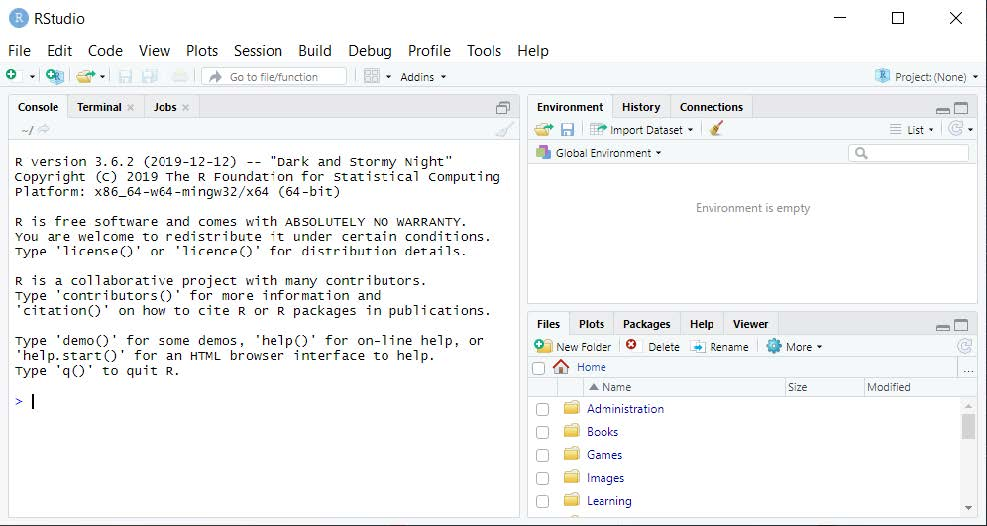
\includegraphics[width=\linewidth]{Files/Images/setup1.jpg}
\end{minipage} \\
\\
\bigskip

\begin{minipage}{0.5\textwidth}
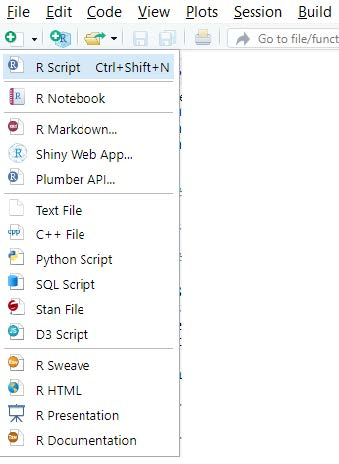
\includegraphics[width=.4\linewidth]{Files/Images/setup2.jpg}
\end{minipage}%
\hfill%
\begin{minipage}{0.4\textwidth}
\textit{2. Press the “New” menu button and choose
“R Script”, or press Ctrl ( $\cmd$ ) + Shift + N to
open a new \texttt{R} script.}
\end{minipage} \\
\\
\bigskip

\begin{minipage}{0.4\textwidth}
\textit{3. You can now write and run your
own code in the newly opened
\texttt{R} script. Select all code you
want to execute and press
Ctrl ( $\cmd$ ) + Enter or "Run" to run.}
\end{minipage}%
\hfill%
\begin{minipage}{0.55\textwidth}
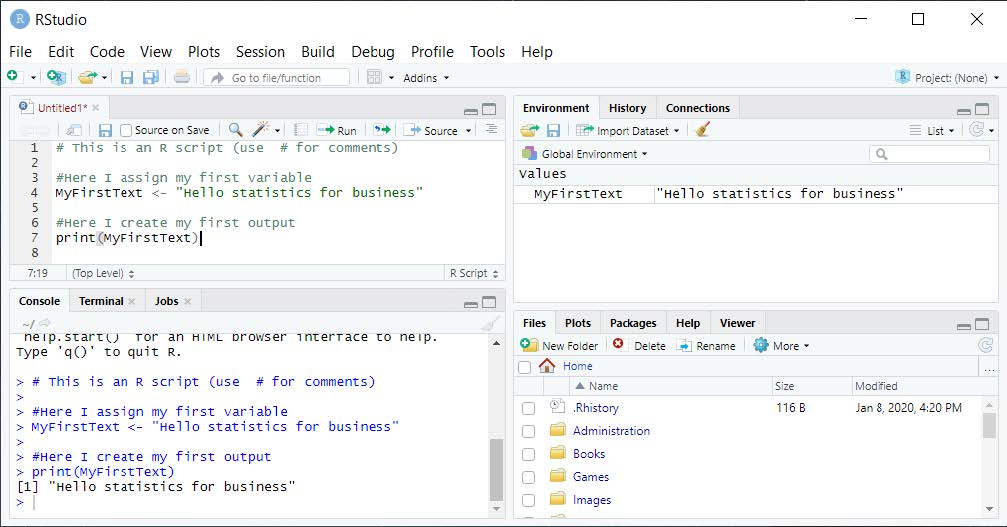
\includegraphics[width=\linewidth]{Files/Images/setup3.jpg}
\end{minipage} \\
\\
\bigskip
                        \clearpage
\vspace*{2cm}
\fancyhf[rh]{}
\begin{center}
    \textit{Probability theory is nothing but common sense reduced to calculation. \\
    \vspace*{0.5cm}
    - Pierre-Simon Laplace (1749 - 1827)}
\end{center}                                    \clearpage
\fancypagestyle{plain}{\fancyhf[rh]{}}\pagestyle{plain}
\tableofcontents                                                                \clearpage
\fancypagestyle{plain}{\fancyhf[rh]{{\fontsize{12}{14}\selectfont\textit{\nouppercase{\rightmark}}}}}\pagestyle{plain}
\addtocontents{toc}{\protect\vspace{10pt}}
\section{Introduction to the workbook}

In this introduction some basic principles are defined that are followed throughout the workbook to guide you through discovering the business potential of statistics using \texttt{R}. Here follows a summation of the different sections that you will come across while working through the various chapters. \\

\bigskip

\textit{Learning objectives} \\

Every chapter has specific learning objectives that give you an initial impression about what you will learn in the assignments of that chapter. The learning objectives also provide a good measurement of your ability after finishing the chapter, since you can check whether you master the learning objectives. \\

The learning objectives are shown at the beginning of each chapter in a {\color{learningobjectives} \fontfamily{pcr}\selectfont \textbf{yellow}} box. \\

\emptylearningobjectives \\

\textit{Exercises by hand} \\

\begin{minipage}{0.85\textwidth}
Fancy some mathematical exercise? When you see the icon to the right you know that you will be expected to perform calculations by hand (or by the use of a simple calculator). For example, you may get asked to calculate the mean of a small data set for an assignment.
\end{minipage}%
\hfill%
\begin{minipage}{0.1\textwidth}

\includegraphics[width=\linewidth]{Files/Images/pencilhand.pdf}
\end{minipage} \\
\\
\bigskip

\textit{Exercises in R} \\ 

\begin{minipage}{0.85\textwidth}
The icon to the right is shown when it is time to start programming in \texttt{R}. You may warm up your programming fingers, since you will be asked to write and run your own code in the assignments that follow. 
\end{minipage}%
\hfill%
\begin{minipage}{0.1\textwidth}

\includegraphics[width=\linewidth]{Files/Images/displaycode.pdf}
\end{minipage} \\
\\
\bigskip 

\textit{Hints} \\

\begin{minipage}{0.85\textwidth}
When you see the icon to the right it means that you will be given a hint for that question. Hints can be useful if you do not know how to get started with an assignment. Pay close attention to these hints, as they may also guide your attention to important aspects that can be easily overlooked.
\end{minipage}%
\hfill%
\begin{minipage}{0.1\textwidth}

\includegraphics[width=\linewidth]{Files/Images/lightbulb.pdf}
\end{minipage}

\clearpage

\textit{Statistical concepts} \\ 

Various important statistical concepts will present itself during the assignments. These statistical concepts are highlighted in \concept{red} and can be found all over the text of the assignments. When these concepts can be calculated, their formulas can often be found in the formula sheet on page~\pageref{formulasheet}. An example such an important statistical concept can be the mean. \\

\concept{mean} \\ 

\bigskip

\textit{Data sets} \\

The color \dataset{green} is used to indicate the name of a data set that can be found in the online resources accompanying this workbook. For example, you might be asked to read a data set into \texttt{R} for further use in an assignment. \\

\dataset{example.csv} \\

\bigskip 

\textit{R code} \\ 

\texttt{R} code in the assignments is displayed in \rcode{blue}. These short lines of kind of code are generally used in the assignments to highlight objects or variables that exist in the current \texttt{R} session. They might also provide information on certain functions to use on an \texttt{R} object. \\

\rcode{View(dataset)} \\ 

\bigskip

\textit{R code blocks} \\ 

\texttt{R} code blocks are used in the assignments to indicate \texttt{R} code that should to be run together. Copy this code into your script in \texttt{RStudio} and select all of the code to run at it at once. Be sure to do this at all times, as running these lines of code individually may influence your results drastically. \\

\codeblock{x <- c(1, 5, 8, 3) \\ mean(x) }
                  \clearpage

% Chapters
\addtocontents{toc}{\protect\vspace{10pt}}
\section{Chapter 1: Descriptive statistics}

\learningobjectives{
    \item Calculating the mean, mode, median, quartiles and range by hand 
    \item Get started with \texttt{R}: set the working directory, inspect and load data
    \item Calculating the mean, mode, median and range in R
}

% To add an assignment to the chapter, create a file in the folder "Assignments" and insert the link below

%%%%%%%%%%%%%%%%%%%%%%%%%%%%%%%%%%%%%%%%%%%%%%%%%%%%%%%%%%%%%%%%%%%%%%%%%%%
% Assignment 1.1: Descriptive statistics by hand
%%%%%%%%%%%%%%%%%%%%%%%%%%%%%%%%%%%%%%%%%%%%%%%%%%%%%%%%%%%%%%%%%%%%%%%%%%%

\handassignment{Assignment 1.1: Descriptive statistics by hand}


Calculate by hand (or by the use of a pocket calculator) the

\begin{itemize}
    \item \concept{mean} 
    \item \concept{mode}
    \item \concept{median}
    \item \concept{range}
    \item \concept{lower and upper quartiles}
    \item \concept{interquartile range}
\end{itemize}

For the following data sets: \\

\question{
    1.1 a
}{
    2\hspace{.3cm}7\hspace{.3cm}4\hspace{.3cm}5\hspace{.3cm}8\hspace{.3cm}10\hspace{.3cm}10\hspace{.3cm}7\hspace{.3cm}9\hspace{.3cm}2\hspace{.3cm}8\hspace{.3cm}8\hspace{.3cm}9\hspace{.3cm}4\hspace{.3cm}6
}
\vspace*{-.4cm} \\
\question{
    1.1 b
}{
    7\hspace{.3cm}7\hspace{.3cm}6\hspace{.3cm}5\hspace{.3cm}2\hspace{.3cm}1\hspace{.3cm}3\hspace{.3cm}7\hspace{.3cm}5\hspace{.3cm}9\hspace{.3cm}9\hspace{.3cm}10
}

\emptyanswerbox{
1.1a
}{ 
Mean: \quad \shortanswerline \hspace{.5cm} \quad Range: \qquad \qquad \qquad \qquad \shortanswerline
            \answerbreak
            Mode: \quad \shortanswerline \hspace{.4cm} \quad Lower quartile: \qquad \quad \shortanswerline
            \answerbreak
            Median: \shortanswerline \hspace{.4cm} \quad Upper quartile: \qquad \quad \shortanswerline
            \answerbreak
            \hspace*{6.1cm} \quad Interquartile range: \shortanswerline}
            
\emptyanswerbox{
1.1b
}{  Mean: \quad \shortanswerline \hspace{.5cm} \quad Range: \qquad \qquad \qquad \qquad \shortanswerline
            \answerbreak
            Mode: \quad \shortanswerline \hspace{.4cm} \quad Lower quartile: \qquad \quad \shortanswerline
            \answerbreak
            Median: \shortanswerline \hspace{.4cm} \quad Upper quartile: \qquad \quad \shortanswerline
            \answerbreak
            \hspace*{6.1cm} \quad Interquartile range: \shortanswerline}

\clearpage % Page break

\question{
    1.1 c
}{
    Describe which question (1.1a or 1.1b) was more difficult to calculate and why.
}

\fourlineanswerbox{1.1c} 

\question{
    1.1 d
}{
    Are these data sets \concept{positively skewed} or \concept{negatively skewed}? Circle the correct answer and explain why you chose this answer using the relation between the \concept{mean}, the \concept{median}, and the \concept{mode}.
}

\emptyanswerbox{
1.1d
}{
These data sets are \textbf{positively} / \textbf{negatively} skewed.
\answerskip
Explanation:
\answerskip
\rule{\textwidth}{0.4pt}
\answerbreak
\rule{\textwidth}{0.4pt}
\answerbreak
\rule{\textwidth}{0.4pt}
}

\clearpage % Page break 
%%%%%%%%%%%%%%%%%%%%%%%%%%%%%%%%%%%%%%%%%%%%%%%%%%%%%%%%%%%%%%%%%%%%%%%%%%%
% Assignment 1.2: Descriptive statistics of small data sets in R
%%%%%%%%%%%%%%%%%%%%%%%%%%%%%%%%%%%%%%%%%%%%%%%%%%%%%%%%%%%%%%%%%%%%%%%%%%%

\rassignment{Assignment 1.2: Descriptive statistics of small data sets in R}

This assignment assumes you opened a new script in the code editor in
\texttt{RStudio}. Write and run your own code to answer the following questions. \\

In R, a one-dimensional row of numbers is represented by a \rcode{vector}. \\

\question{
    1.2 a
}{
    Use the \rcode{c()} function to enter the numbers from assignment 1.1a in a new vector called \rcode{dataset1}. Next, run the following code in \texttt{R} and explain what you see.
}

\codeblock{View(dataset1)}

\hint{Hint 1.1: Check Part I of the R help for more information on how to make a \rcode{vector}.}

\rcodeanswersmall{1.2a}
\twolineanswerbox{1.2a}

\question{
    1.2 b
}{
    Write and run your own code in R to find the \concept{mean}, \concept{mode}, \concept{median}, and \concept{range} for the vector \rcode{dataset1}. Compare your answers with those of assignment 1.1a.
}

\hint{Hint 1.2: Check part IV of the R help on page~\pageref{rhelp} for descriptive statistics functions.}
\hint{Hint 1.3: There is no \concept{mode} function in R, but you can find the mode in a frequency \rcode{table}.}

\rcodeanswersmall{1.2b}

\clearpage % Page break

\emptyanswerbox{
1.2b
}{  Mean: \quad \shortanswerline \hspace{.5cm} \quad Median: \quad \quad \shortanswerline
            \answerskip
            Mode: \quad \shortanswerline \hspace{.5cm} \quad Range: \qquad \quad \shortanswerline}

\question{
    1.2 c
}{
    Run the following code in \texttt{R} and explain what you see.
}

\codeblock{quantile(dataset1, type = 6)}
\twolineanswerbox{1.2c}

\question{
1.2 d
}{
Use the \rcode{c()} function to create a vector \rcode{dataset2} with the data from assignment 1.1b and find the \concept{mean}, \concept{mode}, \concept{median}, \concept{range}, and \concept{quartiles} for these data. Compare your answers with those of assignment 1.1b.
}

\rcodeanswersmall{1.2d}

\emptyanswerbox{
    1.2d
}{  
Mean: \quad \shortanswerline \hspace{.5cm} \quad Range: \qquad \qquad \qquad \qquad \shortanswerline
            \answerbreak
            Mode: \quad \shortanswerline \hspace{.4cm} \quad Lower quartile: \qquad \quad \shortanswerline
            \answerbreak
            Median: \shortanswerline \hspace{.4cm} \quad Upper quartile: \qquad \quad \shortanswerline
}
            
\clearpage % Page break
%%%%%%%%%%%%%%%%%%%%%%%%%%%%%%%%%%%%%%%%%%%%%%%%%%%%%%%%%%%%%%%%%%%%%%%%%%%
% Assignment 1.2: Descriptive statistics of larger data sets in R
%%%%%%%%%%%%%%%%%%%%%%%%%%%%%%%%%%%%%%%%%%%%%%%%%%%%%%%%%%%%%%%%%%%%%%%%%%%

\rassignment{Assignment 1.3: Descriptive statistics of larger data sets in R}

For this assignment, you need the \dataset{bloodPressure.csv} data set that you can download from the online resources. This data set contains measurements of the age, blood pressure, cholesterol level, gender, and description of a random selection of people. It is normally used to look for relationships between these variables. Note that this is fake data and does not contain actual measurements. \\

Let’s start with importing the data set (which is available in the online resources) into \texttt{R}. \\

\question{
    1.3 a
}{
    Inspect and run the following code in \texttt{R} to import the blood pressure data and store it in the object \rcode{dataset3}. Explain how the code works and describe what the \dataset{bloodPressure.csv} file contains.
}

\codeblock{dataset3 <- read.csv(file.choose())}
\twolineanswerbox{1.3a}

This method of importing data can be a lot of work if there are many files or if the script will be run many times. Faster methods exist though, for example by providing the full file path. \\

\question{
    1.3 b
}{
    Describe and test ways this code can be improved to make importing a file easier.
}

\hint{Hint 1.4: Look at Part I of the R help to find out more functions for importing data.}

\twolineanswerbox{1.3b} \\
\rcodeanswersmall{1.3b}

\clearpage % Page break

The functions you used for descriptive statistics on the small data sets in assignment 1.1 can also be applied to the data set that is currently stored in \rcode{dataset3}. \\

\question{
    1.3 c
}{
    Find the \concept{mean}, \concept{mode}, \concept{median}, \concept{range}, and \concept{quartiles} for the column \rcode{Age} in \rcode{dataset3}. Describe this variable in running text using these statistics.
}

\hint{Hint 1.5: First find out how to extract (index) a specific column in a data frame using the \rcode{\$} sign.}

\rcodeanswermedium{1.3c}
\fourlineanswerbox{1.3c}

For large data sets, it becomes a lot of work finding the \concept{mode} in a frequency table each time. It is possible to import a package into the \texttt{R} session that contains a function for calculating the \concept{mode} automatically. However, it is also possible to create a function that calculates the \concept{mode} ourselves. \\

Run the following lines of \texttt{R} code together: \\

\codeblock{getMode <- function(x)\{ \\
  \hspace*{10pt} uniqx <- unique(x) \\
  \hspace*{10pt} uniqx[which.max(tabulate(match(x, uniqx)))] \\
\}
}

You have now created your first \texttt{R} function and you will see it displayed separately in the \texttt{R} environment. This function will give you the \concept{mode} for any \textbf{numeric} vector or column. It works by first extracting all unique values, counting their frequency, and then selecting the value with the highest frequency. Note that you can use this function, but will not be required to understand or make functions like this. However, for the interested reader, part III of the R help contains more information on how to create your own functions. \\

\clearpage % Page break

\question{
    1.3 d
}{
    Use the new \rcode{getMode()} function to determine the \concept{mode} for column \rcode{Age} in \rcode{dataset3} and check if it is consistent with your answer for assignment 1.3c.
}

\rcodeanswertiny{1.3d}
\emptyanswerbox{
    1.3d
}{
    Mode: \shortanswerline
}

\question{
    1.3 e
}{
    Find the \concept{mean}, \concept{mode}, \concept{median}, \concept{range}, and \concept{quartiles} for the column \rcode{BloodPressure} in \rcode{dataset3}. Also use the new \rcode{getMode()} function.
}

\rcodeanswermedium{1.3e}
\emptyanswerbox{
    1.3e
}{
    Mean: \quad \shortanswerline \hspace{.5cm} \quad Range: \qquad \qquad \qquad \qquad \shortanswerline
            \answerbreak
            Mode: \quad \shortanswerline \hspace{.4cm} \quad Lower quartile: \qquad \quad \shortanswerline
            \answerbreak
            Median: \shortanswerline \hspace{.4cm} \quad Upper quartile: \qquad \quad \shortanswerline
}

\question{
    1.3 f
}{
    Is the distribution of the values in the \rcode{BloodPressure} column \concept{positively skewed} or \concept{negatively skewed}? Explain your answer using the relation between the \concept{mean}, \concept{median}, and \concept{mode}.
}

\emptyanswerbox{
1.1f
}{
These data sets are \textbf{positively} / \textbf{negatively} / \textbf{not} skewed.
\answerskip
Explanation:
\answerskip
\rule{\textwidth}{0.4pt}
\answerbreak
\rule{\textwidth}{0.4pt}
\answerbreak
\rule{\textwidth}{0.4pt}
}

\clearpage

\question{
    1.3 g
}{
    Determine the \concept{variance} and \concept{standard deviation} for the column \rcode{Cholestrol} in \rcode{dataset3}.
}

\rcodeanswersmall{1.3g}
\emptyanswerbox{
    1.3g
}{
    Variance: \qquad \qquad \qquad \shortanswerline
    \answerskip
    Standard deviation: \shortanswerline
}

\question{
    1.3 h
}{
    Validate the relation between the \concept{variance} and the \concept{standard deviation} by performing a calculation in \texttt{R}.
}

\rcodeanswertiny{1.3h}

\clearpage % Page break
          \clearpage
\addtocontents{toc}{\protect\vspace{10pt}}
\section{Chapter 2: Creating graphs from data}

\learningobjectives{
    \item Creating a histogram by hand and in R
    \item Creating and modifying a scatter plot in R
    \item Creating and modifying a line plot in R
    \item Creating a box plot in R
}

% To add an assignment to the chapter, create a file in the folder "Assignments" and insert the link below

%%%%%%%%%%%%%%%%%%%%%%%%%%%%%%%%%%%%%%%%%%%%%%%%%%%%%%%%%%%%%%%%%%%%%%%%%%%
% Assignment 2.1: Creating a histogram by hand
%%%%%%%%%%%%%%%%%%%%%%%%%%%%%%%%%%%%%%%%%%%%%%%%%%%%%%%%%%%%%%%%%%%%%%%%%%%

\handassignment{Assignment 2.1: Creating a histogram by hand}

Suppose that you have the following set of numbers: \\

\begin{center}
\hspace{0.3cm}1.5\hspace{0.3cm}5.5\hspace{0.3cm}1.7\hspace{0.3cm}7.2\hspace{0.3cm}1.2\hspace{0.3cm}7.9\hspace{0.3cm}1.4\hspace{0.3cm}3.6\hspace{0.3cm}3.1\hspace{0.3cm}3.8\hspace{0.3cm}5.9\hspace{0.3cm}3.6\hspace{0.3cm}5.1\hspace{0.3cm}3.2\hspace{0.3cm}7.1
\end{center}

\question{
    2.1 a
}{
    For each of the ranges given below, find out their \concept{frequency} in the data above.
}

\emptyanswerbox{
    2.1a
}{
    \begin{center}
    \begin{tabular}{|c|c|c|c|}
    \hline
    0 to 2 & 2 to 4 & 4 to 6 & 6 to 8 \tstrut\bstrut\\
    \hline
    & & & \\
    Frequency:\hspace*{2pt}\rule{0.8cm}{0.4pt}  & Frequency:\hspace*{2pt}\rule{0.8cm}{0.4pt} & Frequency:\hspace*{2pt}\rule{0.8cm}{0.4pt} & Frequency:\hspace*{2pt}\rule{0.8cm}{0.4pt} \bstrut\\
    \hline
    \end{tabular}
    \end{center}
}

\question{
    2.1 b
}{
    Draw the histogram for these data by hand. The name of the \textit{x-axis} should represent the range of values, and the name of the \textit{y-axis} should represent the \concept{frequency} of the values that fall in the ranges of assignment 2.1a.
}

\emptyanswerbox{
    2.1 b
}{
    \vspace*{-0.5cm}
    \begin{center}
    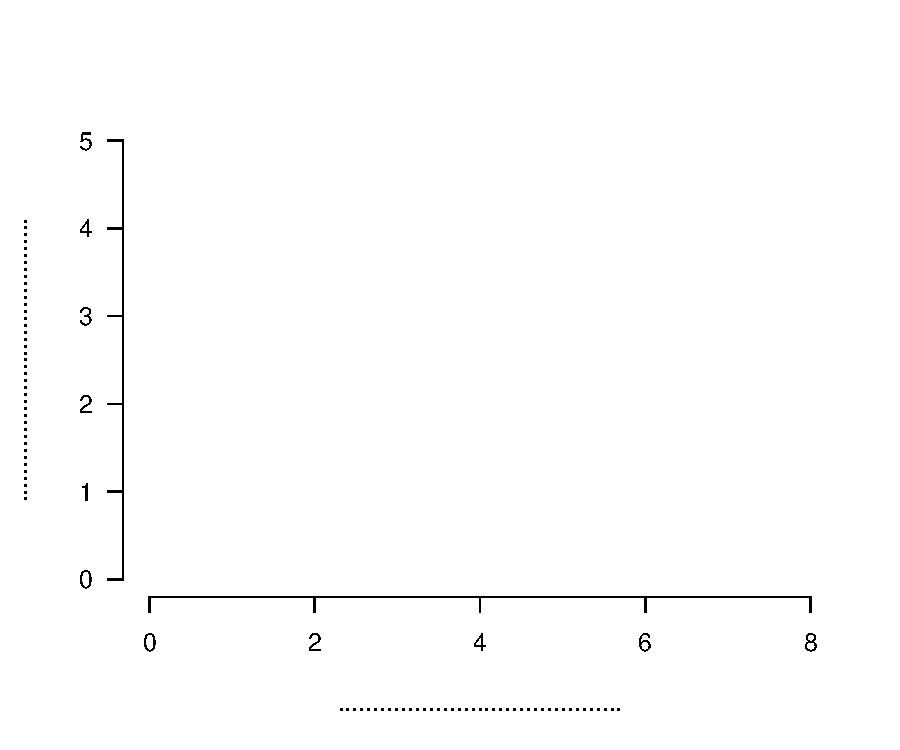
\includegraphics[height = 7cm]{Files/Images/emptyHistogram.pdf}
    \end{center}
}

\clearpage % Page break
%%%%%%%%%%%%%%%%%%%%%%%%%%%%%%%%%%%%%%%%%%%%%%%%%%%%%%%%%%%%%%%%%%%%%%%%%%%
% Assignment 2.2: Creating and modifying a histogram in R
%%%%%%%%%%%%%%%%%%%%%%%%%%%%%%%%%%%%%%%%%%%%%%%%%%%%%%%%%%%%%%%%%%%%%%%%%%%

\rassignment{Assignment 2.2: Creating and modifying a histogram in R}

\question{
    2.2 a
}{
    Take the numbers from assignment 2.1a and use the \rcode{c()} function to enter these numbers in a vector called \rcode{dataset4}. Next, run the following code in \texttt{R} and explain what you see.
}

\codeblock{hist(dataset4)}

\twolineanswerbox{2.2a}

\question{
    2.2 b
}{
    The graph resulting from the command in 2.2a is not the same as the histogram that you drew in assignment 2.1b. What is the difference between the graph from 2.2a and your graph from 2.1b? 
}

\twolineanswerbox{2.2b}

\question{
    2.2 c
}{
    Try to replicate your \underline{exact} histogram from 2.1b in \texttt{R}. This requires that you specify the \rcode{breaks} argument after a comma in the \rcode{hist()} function. 
}

\hint{Hint 2.1: You can find more information on the \rcode{hist()} function by running \rcode{?hist}.}

\rcodeanswertiny{2.2c}

\question{
    2.2 d
}{
    Give your histogram a different color by adding and changing the \rcode{col} argument after the comma. Improve your histogram further by changing the \textit{x-axis} name, the main title, and the rotation of the \textit{y-axis} labels by adding more arguments.
}

\hint{Hint 2.2: Check Part II of the R help for additional arguments to the \rcode{hist()} function.}

\rcodeanswersmall{2.2d}

\question{
    2.2 e
}{
    Calculate the \concept{mean} and \concept{median} of the values of \rcode{dataset4}. Is the distribution of \rcode{dataset4} \concept{negatively skewed} or \concept{positively skewed}? Explain your answer using the relation between the \concept{mean} and the \concept{median}.
}

\emptyanswerbox{
    2.2e
}{
    These data sets are \textbf{positively} / \textbf{negatively} / \textbf{not} skewed.
    \answerskip
    Explanation:
    \answerskip
    \rule{\textwidth}{0.4pt}
    \answerbreak
    \rule{\textwidth}{0.4pt}
    \answerbreak
    \rule{\textwidth}{0.4pt}
}

\clearpage % Page break
%%%%%%%%%%%%%%%%%%%%%%%%%%%%%%%%%%%%%%%%%%%%%%%%%%%%%%%%%%%%%%%%%%%%%%%%%%%
% Assignment 2.3: Creating and modifying a scatter plot in R
%%%%%%%%%%%%%%%%%%%%%%%%%%%%%%%%%%%%%%%%%%%%%%%%%%%%%%%%%%%%%%%%%%%%%%%%%%%

\rassignment{Assignment 2.3: Creating and modifying a scatter plot in R}

In this assignment you are going to work with a data set that is built into \texttt{R}. \\

The \rcode{data()} function gives you access to all the data sets that are built into \texttt{R}, or that are included with downloaded \texttt{R} packages. For example, you can load a data set called \rcode{swiss} into the environment by running the \texttt{R} code below: \\

\codeblock{data(swiss)} 

The data are imported as an object called \rcode{swiss}, which you can now also see in the environment. This particular data set contains some socio-economic indicators for each of 47 French-speaking provinces of Switzerland. In this assignment, you will focus on the column \rcode{Education} (the percentage education beyond primary school) and the column \rcode{Agriculture} (the percentage of males involved in agriculture as an occupation). \\

\question{
    2.3 a
}{
    Extract the values of the two columns using the \rcode{\$} sign and store them in two new variables called \rcode{education} and \rcode{agriculture}.
}

\hint{Hint 2.3: You can check the R environment to see the names of the objects that you have currently stored.}

\rcodeanswertiny{2.3a}

\question{
    2.3 b
}{
    Use the \rcode{plot()} function to create a scatter plot of the two variables. Place the percentage of education beyond primary school on the \textit{x-axis} and the percentage of males involved in agriculture as an occupation on the \textit{y-axis}. Rename your axis labels to match the content of the graph.
}

\rcodeanswerlarge{2.3b}

\clearpage % Page break

\question{
    2.3 c
}{
    Looking at the scatter plot, what can you globally say about the relation between the percentage of education beyond primary school and the percentage of males involved in agriculture as an occupation in the French-speaking provinces of Switzerland? 
}

\twolineanswerbox{2.3c}

\question{
    2.3 d
}{
    Give the points in your scatter plot a different color by changing the \rcode{col} argument after the comma. Improve the graph further by changing the main title, the rotation of the \textit{y-axis} labels, the shape of the points, and removing the outer lines.
}

\rcodeanswerlarge{2.3d}

\clearpage % Page break
%%%%%%%%%%%%%%%%%%%%%%%%%%%%%%%%%%%%%%%%%%%%%%%%%%%%%%%%%%%%%%%%%%%%%%%%%%%
% Assignment 2.4: Creating and modifying a line plot in R
%%%%%%%%%%%%%%%%%%%%%%%%%%%%%%%%%%%%%%%%%%%%%%%%%%%%%%%%%%%%%%%%%%%%%%%%%%%

\rassignment{Assignment 2.4: Creating and modifying a line plot in R}

In this assignment, you are going to create a line plot of the daily closing prices of some major European stock indices: Germany DAX, Switzerland SMI, France CAC, and UK FTSE. \\

You can load this data set by running the code below: \\

\codeblock{data(EuStockMarkets) \\
            stockData <- data.frame(EuStockMarkets)
}

The data is now loaded into the environment as the \rcode{EuStockMarkets} data set and immediately transformed to the \rcode{stockData} data set (this is because of technical reasons as the original data is in a time-series format). In this assignment, you will work with the \rcode{stockData} data set. \\

\question{
    2.4 a
}{
    Create a line plot where the closing price of the DAX stock is displayed over time. Give your plot appropriate \textit{x-axis} and \textit{y-axis} names.
}

\rcodeanswersmall{2.4a}

\question{
    2.4 b
}{
    Find a function to add a separate line for the closing price of the SMI stock in red. You may try to add the other stocks as well using this function, but remember to adjust the \textit{y-axis} accordingly so that all the lines are all displayed decently.
}

\hint{Hint 2.4: Do \underline{not} use the \rcode{plot()} function to add a line to an already existing plot.}

\rcodeanswersmall{2.4 b}

\clearpage % Page break
%%%%%%%%%%%%%%%%%%%%%%%%%%%%%%%%%%%%%%%%%%%%%%%%%%%%%%%%%%%%%%%%%%%%%%%%%%%
% Assignment 2.5: Creating a box plot in R
%%%%%%%%%%%%%%%%%%%%%%%%%%%%%%%%%%%%%%%%%%%%%%%%%%%%%%%%%%%%%%%%%%%%%%%%%%%

\rassignment{Assignment 2.5: Creating a box plot in R}

For this next assignment, let’s return to the \rcode{swiss} data set. More specifically, you will now have to focus on the values that are stored in the separate variable \rcode{agriculture}. \\

\question{
    2.5 a
}{
    Find out the \concept{minimum}, \concept{lower quartile}, \concept{median}, \concept{upper quartile}, and \concept{maximum} of the \rcode{agriculture} variable.
}

\rcodeanswersmall{2.5a}

\emptyanswerbox{
    2.5a
}{
    Minimum: \quad \shortanswerline \quad Upper quartile: \shortanswerline
            \answerskip
            Median: \quad\hspace*{7pt} \shortanswerline \quad Lower quartile: \shortanswerline
            \answerskip
            Maximum: \quad \shortanswerline
}

\question{
    2.5 b
}{
    Create a boxplot of the \rcode{agriculture} variable.
}

\rcodeanswertiny{2.5b}

\question{
    2.5 c
}{
    Run the following code in \texttt{R} and explain the table output. How does the code work?
}

\codeblock{educationLevel <- rep(\textquotesingle2.Medium\textquotesingle, 47)\\
educationLevel[education <= 6] = \textquotesingle1.Low\textquotesingle\\
educationLevel[education >= 12] = \textquotesingle3.High\textquotesingle\\
table(educationLevel)
}

\twolineanswerbox{2.5c}

\clearpage % Page break

\question{
    2.5 d
}{
    Create a box plot using the \texttt{R} code below and explain what you see.
}

\codeblock{boxplot(agriculture {\raise.17ex\hbox{$\scriptstyle\sim$}} educationLevel)}

\twolineanswerbox{2.5d}

\clearpage % Page break       \clearpage
\addtocontents{toc}{\protect\vspace{10pt}}
\section{Chapter 3: Confidence intervals and hypothesis testing}

\learningobjectives{
    \item Confidence interval and hypothesis testing by hand
    \item Testing the homogeneity of variance by hand
    \item Calculating confidence intervals for the mean and testing for normality
    \item Inspect and test the normality of a sample in R
    \item Using R to inspect and test the homogeneity of variance
}

% To add an assignment to the chapter, create a file in the folder "Assignments" and insert the link below

%%%%%%%%%%%%%%%%%%%%%%%%%%%%%%%%%%%%%%%%%%%%%%%%%%%%%%%%%%%%%%%%%%%%%%%%%%%
% Assignment 3.1: Confidence interval and hypothesis testing by hand
%%%%%%%%%%%%%%%%%%%%%%%%%%%%%%%%%%%%%%%%%%%%%%%%%%%%%%%%%%%%%%%%%%%%%%%%%%%

\handassignment{Assignment 3.1: Confidence interval and hypothesis testing by hand}

A call center with 38 employees handles thousands of calls a day. The company wants to get more insights into the duration of calls and the workload of the employees. On a day with a total of 4513 calls, the company decides to randomly pick 100 calls and measure how long they take. The \concept{mean} call duration for this sample is 145 seconds with a \concept{standard deviation} of 25 seconds. The call center wants to use this information to estimate the \concept{mean} call duration for that day. \\

\question{
    3.1 a
}{
    Write down the relevant information from this case. Use the symbols $N$, $n$, $\bar{x}$, $s$, $\sigma$, and $\mu$.
}

\hint{Hint 3.1: Not all symbols are known and some should be left empty.}

\emptyanswerbox{
    3.1a
}{
        $N$: \shortanswerline \hspace{1cm} \quad $s$: \shortanswerline
            \answerbreak
            $n$: \shortanswerline \hspace{1cm} \quad $\sigma$: \shortanswerline
            \answerbreak
            $\bar{x}$: \shortanswerline \hspace{1cm} \quad $\mu$: \shortanswerline
}

\question{
    3.1 b
}{
    What is the best estimate of the \concept{mean} call duration ($\mu$) based on this sample?
}

\emptyanswerbox{
    3.1b
}{
    $\mu = $\shortanswerline    
    \answerskip
    Explanation:
    \answerskip
    \rule{\textwidth}{0.4pt}
}

\clearpage % Page break

\question{
    3.1 c
}{
    Calculate the \concept{standard error} of the mean ($SE_\mu$) based on this sample.
}

\hint{Hint 3.2: Check the formula sheet to find out how to calculate $SE_\mu$.}

\emptyanswerbox{
    3.1c
}{
    $SE_\mu = $\shortanswerline    
    \answerskip
    Calculation:
    \answerskip
    \rule{\textwidth}{0.4pt}
}

\question{
    3.1 d
}{
    Calculate the 99\% \concept{confidence interval} for the mean call duration.
}

\hint{Hint 3.3: You can find the formula for the \concept{lower bound}, \concept{upper bound} and \concept{z-value} in the formula sheet.}

\emptyanswerbox{
    3.1d
}{
    z-value: \qquad \shortanswerline    
    \answerskip
    Calculation: \mediumanswerline
    \answerskip
    \answerskip
    Lower bound: \shortanswerline    
    \answerskip
    Calculation: \mediumanswerline
    \answerskip
    \answerskip
    Upper bound: \shortanswerline    
    \answerskip
    Calculation: \mediumanswerline
    \answerskip
}

The manager of the call center does not really care about the \concept{lower bound} and he does not require such high confidence. He just wants to make sure the average workload per employee is not too high, because otherwise he is forced by employment laws to hire more people. He calculated that if the \concept{mean} call duration is below 150 seconds the workload is acceptable, and wants to use this sample to show with 95\% confidence that the \concept{mean} call duration is below 150 seconds. \\

\clearpage % Page break

\question{
    3.1 e
}{
    Write down the hypotheses $H_0$ and $H_1$ for the manager’s test. What is the value of $\mu_0$? Also describe $\mu_0$ for this case. 
}

\hint{Hint 3.4: This is a one-sided test. Consider this when you formulate the hypotheses.}

\emptyanswerbox{
    3.1e
}{
    $\mu_0$: \shortanswerline    
    \answerskip
    $H_0$: \shortanswerline \hspace{5cm} $H_1$: \shortanswerline
}

\question{
    3.1 f
}{
    Do you need the \concept{lower bound} or the \concept{upper bound} of the \concept{confidence interval} for this test? Calculate this bound. 
}

\emptyanswerbox{
    3.1f
}{
    ........ bound: \shortanswerline    
    \answerskip
    Calculation: \qquad \hspace*{5pt} \mediumanswerline
}

\question{
    3.1 g
}{
    Draw the conclusion for the manager. Include the following four elements:
    \begin{itemize}
        \item[$\square$] Show how the \concept{confidence interval} relates to $\mu_0$.
        \item[$\square$] Discuss whether $H_0$ is rejected or not.
        \item[$\square$] Describe what this tells us about $\mu$ and $\mu_0$.
        \item[$\square$] Describe what type of error is relevant \textit{(type-I or type-II)}.
    \end{itemize}
}

\sixlineanswerbox{3.1g}

\clearpage % Page break
%%%%%%%%%%%%%%%%%%%%%%%%%%%%%%%%%%%%%%%%%%%%%%%%%%%%%%%%%%%%%%%%%%%%%%%%%%%
% Assignment 3.2: Testing for homogeneity of variance by hand
%%%%%%%%%%%%%%%%%%%%%%%%%%%%%%%%%%%%%%%%%%%%%%%%%%%%%%%%%%%%%%%%%%%%%%%%%%%

\handassignment{Assignment 3.2: Testing for homogeneity of variance by hand}

A manufacturer of machines for food processing has created a machine that fills bags with sugar. A machine like this is never perfect and when a 1-kilo bag of sugar is filled there are always small deviations. the actual content of a bag is often a few grams more or less than a kilo. The manufacturer knows these deviations are bigger for new machines but become smaller as the machine is longer used due to better calibration and the smoothing out of the moving parts. To be able to show this to his clients they take a random sample of eight bags of sugar on the first day of the three months the machine is in use and plots the (absolute) weight deviations. \\

The manufacturer wants to use the chart below for a model that shows how much the machine improves over time, but this requires \concept{homogeneity of variances}. The \concept{variance} in month 1 is 0.801 gr, the \concept{variance} in month 2 is 1.113 gr. The \concept{variance} for month 3 has not been calculated yet. \\

\begin{minipage}[t]{0.5\textwidth}
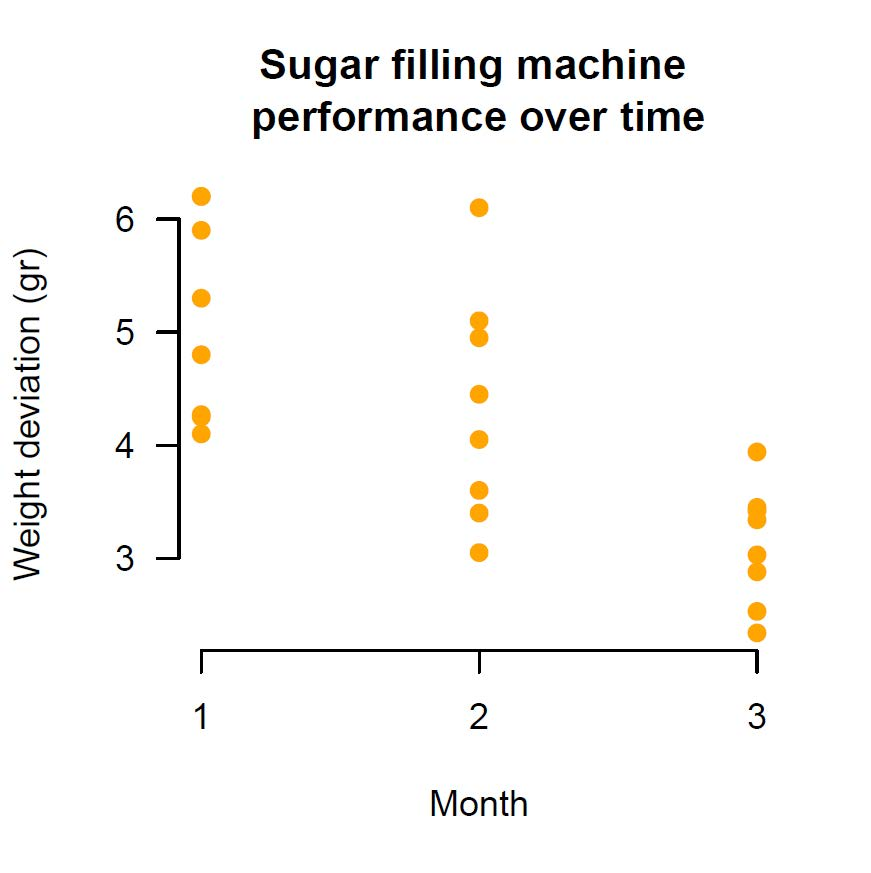
\includegraphics[width=\textwidth]{Files/Images/homogeneityOfVariances.jpg}
\end{minipage}%
\begin{minipage}[t]{0.5\textwidth}
\vspace*{-7cm}
\begin{center}
    \begin{tabular}{|c|c|c|c|}
    \hline 
    $i$ & $x_i$ & $(x_i - \bar{x})$ & $(x_i - \bar{x})^2$ \tstrut\bstrut\\
    \hline
    1 & 3.03 & & \tstrut\bstrut\\
    \hline
    2 & 3.45 & & \tstrut\bstrut\\
    \hline
    3 & 3.94 & & \tstrut\bstrut\\
    \hline
    4 & 2.34 & & \tstrut\bstrut\\
    \hline
    5 & 3.34 & & \tstrut\bstrut\\
    \hline
    6 & 2.53 & & \tstrut\bstrut\\
    \hline
    7 & 2.88 & & \tstrut\bstrut\\
    \hline
    8 & 3.42 & & \tstrut\bstrut\\
    \hline
    \end{tabular}
    \end{center}
    
    $\sum x_i = $  ............. \hspace*{.4cm} $\sum (x_i - \bar{x})^2 = $  ............. \\
    \\
    \hspace*{10pt} $\bar{x} = $ ............. \hspace*{2cm} $s^2 = $  ............. \\
\end{minipage}%

\question{
    3.2 a
}{
    Use the table to the right of the figure to calculate the \concept{variance} $s^2$ for month 3 by filling in the calculations beneath the table.
}

\hint{Hint 3.5: you can find the formula for the \concept{variance} in the formula sheet.}

\emptyanswerbox{
    3.2a
}{
    Variance: \shortanswerline
}   

\question{
    3.2 b
}{
    Calculate \concept{Hartley’s F} (the variance ratio) for the sugar machine data set.
}

\hint{Hint 3.6: you can find the formula for \concept{Hartley’s F} in the formula sheet.}

\clearpage % Page break

\emptyanswerbox{
    3.2b
}{
    Hartley's F: \shortanswerline
}   

\question{
    3.2 c
}{
    Formulate the \concept{null hypothesis} $H_0$ and \concept{alternative hypothesis} $H_1$ to test homogeneity of variance for this case.
}

\hypothesesbox{3.2c}

\question{
    3.2 d
}{
    Determine the \concept{critical value} for Hartley’s F ($F_{\max}$) for the sugar machine data set.
}

\hint{Hint 3.7: Check Table 1 in the formula sheet for the critical values of \concept{Hartley’s F}.}

\emptyanswerbox{
    3.2d
}{
    Hartley's $F_{\max}$: \shortanswerline
}   

\question{
    3.2 e
}{
    Draw the conclusion on the homogeneity of variance for the sugar machine data set. Include the following elements:
    \begin{itemize}
        \item[$\square$] Show how the calculated \concept{Hartley's F} relates to the critical value $F_{max}$.
        \item[$\square$] Discuss whether $H_0$ is rejected or not.
        \item[$\square$] Describe what this tells us about the homogeneity of the three variances.
        \item[$\square$] Describe what type of error is relevant \textit{(type-I or type-II)}.
    \end{itemize}
}

\sixlineanswerbox{3.2e}

\clearpage % Page break
%%%%%%%%%%%%%%%%%%%%%%%%%%%%%%%%%%%%%%%%%%%%%%%%%%%%%%%%%%%%%%%%%%%%%%%%%%%
% Assignment 3.3: Calculating the confidence interval for the mean and
% testing for normality
%%%%%%%%%%%%%%%%%%%%%%%%%%%%%%%%%%%%%%%%%%%%%%%%%%%%%%%%%%%%%%%%%%%%%%%%%%%

\rassignment{Assignment 3.3: Calculating a confidence interval and
testing for normality}

For this assignment, you will need the \dataset{populations.csv} data file, which contains four different \concept{populations} of 10,000 observations called \rcode{P1 - P4}. \\

\question{
    3.3 a
}{
    Use the \rcode{read.csv()} function (and \rcode{setwd()} function if you prefer) to import the data set into an object named \rcode{dataset5}.
}

\rcodeanswertiny{3.3a}

\question{
    3.3 b
}{
    Run the following code in \texttt{R} and explain what it does. Why do you have to use a seed?
}

\codeblock{set.seed(54321) {\color{dataset} \# You can replace 54321 with your own seed number} \\
\\
sample1 <- sample(dataset5\$P1, size = 90)\\
sample2 <- sample(dataset5\$P2, size = 90)\\
sample3 <- sample(dataset5\$P3, size = 90)\\
sample4 <- sample(dataset5\$P4, size = 90)
}

\hint{Hint 3.8: Use R’s help function \rcode{?} to look for the \rcode{sample()} and \rcode{set.seed()} functions.}

\twolineanswerbox{3.3b}

\question{
    3.3 c
}{
    Calculate the \concept{mean} and \concept{standard deviation} for each \concept{sample} and save them into variables \rcode{x1} - \rcode{x4} and \rcode{s1} - \rcode{s4}. Use these results to also calculate the \concept{standard errors} and same them into variables \rcode{se1} - \rcode{se4}.
}

\rcodeanswermedium{3.3c}

\clearpage % Page break

\emptyanswerbox{
    3.3c
}{
    Standard error sample 1: \shortanswerline
    \answerskip
    Standard error sample 2: \shortanswerline
    \answerskip
    Standard error sample 3: \shortanswerline
    \answerskip
    Standard error sample 4: \shortanswerline
}

The \texttt{R} function \rcode{qnorm(p, mean, sd)} returns the \concept{z-value} for \concept{quantile} \rcode{p} from a \concept{normal distribution} with a certain \concept{mean} $\mu$ (\rcode{mean}) and \concept{standard deviation} $\sigma$ (\rcode{sd}). If you do not specify a mean or standard deviation for the function it will assume the standard normal distribution $N(\mu = 0, \sigma = 1)$. \\

\question{
    3.3 d
}{
    Run the following code in \texttt{R} and explain the value that you see. 
}

\codeblock{qnorm(p = 0.95)}

\twolineanswerbox{3.3d}

The \rcode{qnorm()} function cannot return the \concept{z-value} for the two-sided \concept{confidence interval}, but you can work around that by realizing that in a two-sided interval you have to split the risk over both sides of the standard normal distribution. \\

\question{
    3.3 e
}{
    Run the following code in \texttt{R} and explain why you can use the value in \rcode{z} for a two-sided 95\% \concept{confidence interval}. 
}

\codeblock{z <- qnorm(p = 0.975)}

\twolineanswerbox{3.3e}

\question{
    3.3 f
}{
    Calculate the 95\% \concept{confidence interval} for each sample. Store the lower bounds \rcode{lb1} - \rcode{lb4} and store the upper bounds in \rcode{ub1} - \rcode{ub4}.
}

\clearpage % Page break

\rcodeanswermedium{3.3f}

This is a rare case in which you actually have the full \concept{populations}, so you can check if the estimates based on your \concept{samples} are actually close to the real value in the populations. \\

\question{
    3.3 g
}{
    Calculate the actual \concept{population means}, call them \rcode{mu1} - \rcode{mu4}. Next, fill the schema below with all known values for \rcode{ub}, \rcode{x}, \rcode{lb}, and \rcode{mu}. 
}

\rcodeanswermedium{3.3g}

\emptyanswerbox{
    3.3g
}{
    \vspace*{-10pt}
    \begin{center}
    \begin{tabular}{r|c|c|c|c|}
    \multicolumn{1}{c}{} & \multicolumn{1}{c}{\rcode{sample1}} & \multicolumn{1}{c}{\rcode{sample2}} & \multicolumn{1}{c}{\rcode{sample3}} & \multicolumn{1}{c}{\rcode{sample4}} \tstrut\bstrut\\
    \cline{2-5}
    \rcode{ub} & & & & \tstrut\bstrut\\
    \cline{2-5}
    \rcode{x} & & & & \tstrut\bstrut\\
    \cline{2-5}
    \rcode{lb} & & & & \tstrut\bstrut\\
    \cline{2-5}
    \end{tabular}
    \end{center}
    
    \begin{center}
    \begin{tabular}{r|c|c|c|c|}
    \multicolumn{1}{c}{} & \multicolumn{1}{c}{\rcode{P1}} & \multicolumn{1}{c}{\rcode{P2}} & \multicolumn{1}{c}{\rcode{P3}} & \multicolumn{1}{c}{\rcode{P4}} \tstrut\bstrut\\
    \cline{2-5}
    \rcode{mu} & & & & \tstrut\bstrut\\
    \cline{2-5}
    \textit{mu in interval?} & YES / NO & YES / NO & YES / NO & YES / NO \tstrut\bstrut\\
    \cline{2-5}
    \end{tabular}
    \end{center}
}

\question{
    3.3 h
}{
    Are all \concept{population means} inside the interval you calculated?
}

\emptyanswerbox{
    3.3h
}{
    \vspace*{-15pt}
    \begin{center}
        YES / NO
    \end{center}
}

\question{
    3.3 i
}{
    How often do you expect this to happen given the confidence level (95\%) used?
}

\onelineanswerbox{3.3i}

\clearpage % Page break
%%%%%%%%%%%%%%%%%%%%%%%%%%%%%%%%%%%%%%%%%%%%%%%%%%%%%%%%%%%%%%%%%%%%%%%%%%%
% Assignment 3.4: Inspect and test the normality of a sample in R
%%%%%%%%%%%%%%%%%%%%%%%%%%%%%%%%%%%%%%%%%%%%%%%%%%%%%%%%%%%%%%%%%%%%%%%%%%%

\rassignment{Assignment 3.4: Inspecting and testing the normality of a sample in R}

In this assignment you are going to work with an \texttt{R} package called \rcode{car}. Packages are extensions for \texttt{R} created by its community. They contain functions that are not available in the basic \texttt{R} version and can be really useful. There are many packages on the internet, so only use the one you really need and always make sure you use packages from a reliable source (like the official \rcode{CRAN} servers). For clarity, it will be indicated what functions come from what packages in the chapters. If there is no package mentioned, functions come from base \texttt{R}. \\

A package has to be installed once. Run the following code in R to install the car package: \\

\codeblock{install.packages(\textquotesingle car\textquotesingle)}

A package needs to be loaded in \textbf{every script} that uses functions from this package. \\

\codeblock{library(car)}

This assignment assumes you have done assignment 3.3 and therefore have four $n = 90$ samples called \rcode{sample1} - \rcode{sample4} from populations \rcode{P1} - \rcode{P4} from \rcode{dataset5} and calculated the \concept{confidence intervals} for the population means. \\

\question{
    3.4 a
}{
    Create a histogram for each sample in \rcode{sample1} - \rcode{sample4}.
}

\rcodeanswermedium{3.4a}

\question{
    3.4 b
}{ 
    Which samples look like they could have been taken from a \concept{normal distribution}?
}

\threelineanswerbox{3.4b}

\clearpage % Page break

\question{
    3.4 c
}{
    Use this \texttt{R} code (from the \rcode{car} package) to create four \concept{qq-plots} for the four \concept{samples}. 
}

\codeblock{qqPlot(sample1, distribution = \textquotesingle norm\textquotesingle) {\color{dataset}\# qqPlot for sample 1}}

\rcodeanswermedium{3.4c}

\question{
    3.4 d
}{
    Evaluate each \concept{qq-plot} and explain the deviations from the diagonal by referencing features of the histograms. Do the \concept{qq-plots} confirm your answer for question 3.4b?
}

\fourlineanswerbox{3.4c and 3.4d}

\question{
    3.4 e
}{
    Formulate the \concept{null hypothesis} $H_0$  and \concept{alternative hypothesis} $H_1$ for a test of normality in these samples.
}

\hypothesesbox{3.4e}

\question{
    3.4 f
}{
    Use the following \texttt{R} code to perform a \concept{Shapiro-Wilk} normality test on the four samples. Use a confidence level of 99\% and write down the conclusion for each sample.
}

\codeblock{shapiro.test(sample1) {\color{dataset}\# Normality test for sample 1}}

\hint{Hint 3.9: First think about what \concept{p-values} lead to rejecting the \concept{null hypothesis} $H_0$.}

\clearpage % Page break

\rcodeanswersmall{3.4f}
\fourlineanswerbox{3.4f}

In assignment 3.3 you used these \concept{samples} and the \concept{normal distribution} to estimate the \concept{confidence interval} for the \concept{population mean}. You also tested whether the actual population means were inside these intervals, which they almost always were. \\

Now you found out that most of these samples are actually not normally distributed at all. \\

\question{
    3.4 g
}{
    If a sample is not normally distributed, does that mean you cannot use it to estimate the population mean? Explain your answer.
}

\emptyanswerbox{
    3.4g
}{
    When the sample is not normally distributed, the sample \textbf{can} / \textbf{cannot} be used to estimate the population mean.
    \answerskip
    Explanation:
    \answerskip
    \rule{\textwidth}{0.4pt}
    \answerbreak
    \rule{\textwidth}{0.4pt}
    \answerbreak
    \rule{\textwidth}{0.4pt}
}

\clearpage % Page break
%%%%%%%%%%%%%%%%%%%%%%%%%%%%%%%%%%%%%%%%%%%%%%%%%%%%%%%%%%%%%%%%%%%%%%%%%%%
% Assignment 3.5: Using R to inspect and test the homogeneity of variance
%%%%%%%%%%%%%%%%%%%%%%%%%%%%%%%%%%%%%%%%%%%%%%%%%%%%%%%%%%%%%%%%%%%%%%%%%%%

\rassignment{Assignment 3.5: Using R to inspect and test the homogeneity of variance}

In this assignment, you will use the \rcode{iris} data set that is built into \texttt{R}. It is assumed that you have also installed the \rcode{car} package (from assignment 4.4). \\

Run the following code in \texttt{R} to load the \rcode{car} library and load the \rcode{iris} data set into the environment. \\

\codeblock{library(car)\\
data(iris)}

\question{
    3.5 a
}{
    Use the following code to create a \concept{box plot} for the sepal length (\rcode{Sepal.Length}) per flower species (\rcode{Species}). Then rewrite the code to do the same for the sepal width (\rcode{Sepal.Width}) per flower species. 
}

\codeblock{plot(x = iris\$Species, y = iris\$Sepal.Length, \\
     \hspace*{30pt}col = \textquotesingle grey\textquotesingle, main = \textquotesingle Sepal Length\textquotesingle)}
     
\rcodeanswersmall{3.5a}

\question{
    3.5 b
}{
    Visually inspect the graphs for \concept{homogeneity of variance}. What can you say about the spread of the sepal length within the different iris species?
}

\fourlineanswerbox{3.5b}

\question{
    3.5 c
}{
    Formulate the \concept{null hypothesis} $H_0$  and \concept{alternative hypothesis} $H_1$ to test for \concept{homogeneity of variance} in these samples.
}

\hypothesesbox{3.5c}

\clearpage % Page break

\question{
    3.5 d
}{
    Use the (\rcode{car} package) function \rcode{leveneTest()} to test the \concept{homogeneity of variance} for the sepal length and width of the three species. Evaluate the hypotheses with a 90\% confidence. Include the following elements:
    \begin{itemize}
        \item[$\square$] Discuss what the \concept{p-value} is for this test.
        \item[$\square$] Discuss whether $H_0$ is rejected or not.
        \item[$\square$] Describe what this tells us about the homogeneity of the three variances.
        \item[$\square$] Describe what type of error is relevant \textit{(type-I or type-II)}.
    \end{itemize}
}

\hint{Hint 3.10: Look up \rcode{?leveneTest} in R’s help function (it is now also present because you have loaded the \rcode{car} package).}

\rcodeanswertiny{3.5d}
\sixlineanswerbox{3.5d}

\clearpage % Page break

  \clearpage
\addtocontents{toc}{\protect\vspace{10pt}}
\section{Chapter 4: Correlation and regression}

\learningobjectives{
    \item Calculating covariance and correlation by hand
    \item Testing hypotheses about a correlation by hand
    \item Calculating and testing a correlation in R
    \item Testing hypotheses using linear regression in R
    \item Making predictions using linear regression in R
}

% To add an assignment to the chapter, create a file in the folder "Assignments" and insert the link below

%%%%%%%%%%%%%%%%%%%%%%%%%%%%%%%%%%%%%%%%%%%%%%%%%%%%%%%%%%%%%%%%%%%%%%%%%%%
% Assignment 4.1: Calculating covariance and correlation by hand
%%%%%%%%%%%%%%%%%%%%%%%%%%%%%%%%%%%%%%%%%%%%%%%%%%%%%%%%%%%%%%%%%%%%%%%%%%%

\handassignment{Assignment 4.1: Calculating covariance and correlation by hand}

The manager of a local branch of a supermarket chain in the Netherlands has had a bad year last year and wants to improve their sales. Her co-worker has brought up the idea to spend more money on advertising in the neighborhoods that are further away from the store. The co-worker thinks that customers that live further away might visit the supermarket less frequently. He believes that making an effort to attract these people may prove to be profitable for the store. Realizing that her branch currently does not spend a notable amount of money on advertising at all, the manager is interested to know about the \concept{relationship} between the distance a customer lives from the store and the average number of times they visit the store per week. \\

The manager requests her co-worker to ask the customers at his counter some questions when they check out at his counter. He is instructed to ask them a) how many times, on average, they visit the store per week and b) the number of kilometers they live from the store. The co-worker asks eight customers and reports the findings to his manager. \\

\question{
    4.1 a
}{
    What kind of \concept{relationship} do you expect to see? Formulate your answer in terms of the direction of the \concept{relationship}.
}

\twolineanswerbox{4.1a}

The manager sits down with her co-worker, writes down the numbers, and creates a scatter plot of the data. She displays the distance a customer lives from the store (in kilometers) on the \textit{x-axis} and their average number of visits per week on the \textit{y-axis}. 

\clearpage % Page break

\begin{minipage}[t]{0.4\textwidth}
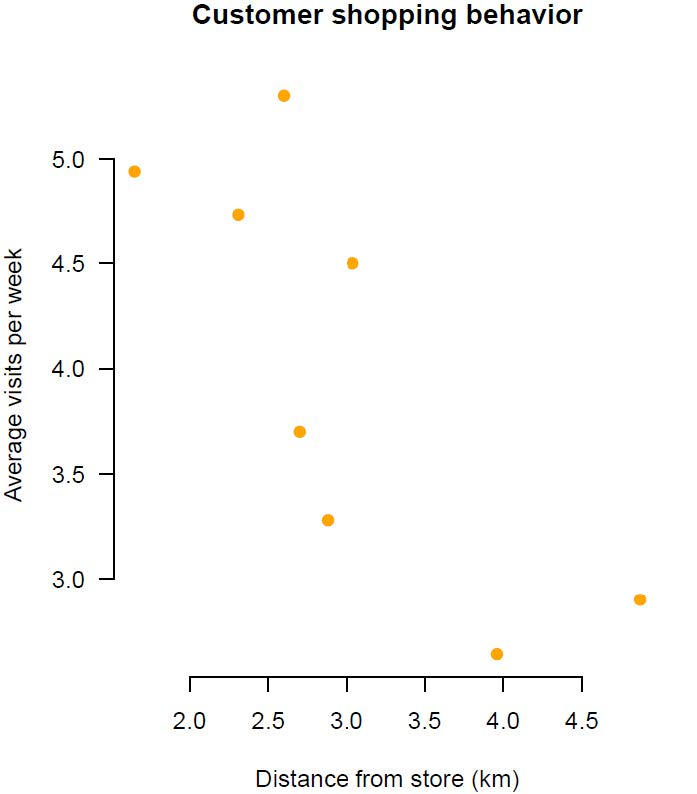
\includegraphics[width=\textwidth]{Files/Images/covariance.jpg}
\end{minipage}%
\begin{minipage}[t]{0.6\textwidth}
\vspace*{-7cm}
\begin{center}
    \begin{tabular}{|c|c|c|c|c|c|}
    \hline 
    $i$ & $x_i$ & $y_i$ & $(x_i - \bar{x})$ & $(y_i - \bar{y})$ & $(x_i - \bar{x})(y_i - \bar{y})$ \tstrut\bstrut\\
    \hline
    1 & 4.87 & 2.90 & & &  \tstrut\bstrut\\
    \hline
    2 & 3.04 & 4.50 & & &  \tstrut\bstrut\\
    \hline
    3 & 1.65 & 4.94 & & &  \tstrut\bstrut\\
    \hline
    4 & 2.88 & 3.28 & & &  \tstrut\bstrut\\
    \hline
    5 & 2.31 & 4.73 & & &  \tstrut\bstrut\\
    \hline
    6 & 3.96 & 2.64 & & &  \tstrut\bstrut\\
    \hline
    7 & 2.70 & 3.70 & & &  \tstrut\bstrut\\
    \hline
    8 & 2.60 & 5.30 & & &  \tstrut\bstrut\\
    \hline
    \end{tabular}
    \end{center}
    
    \hspace*{.5cm} $\bar{x} = $  ............. \hspace*{1cm} $\sum (x_i - \bar{x})(y_i - \bar{y}) = $  ............. \\
    \\
    \hspace*{.5cm} $\bar{y} = $ ............. \hspace*{3.1cm} $n - 1 = $  ............. \\
    \\
    \hspace*{6.5cm} $s_{xy} = $  ............ \\
\end{minipage}%

\question{
    4.1 b
}{
    Use the table above to calculate and fill in the \concept{covariance} $s_{xy}$ between the customer’s distance from the store and their average number of visits per week. 
}

\hint{Hint 4.1: you can find the complete formula for the \concept{covariance} in the formula sheet.}

\question{
    4.1 c
}{
    Interpret the \concept{covariance} from these data. What can you say about the \concept{relationship} between the distance from the store and the average number of visits per week on the basis of this measure?
}

\threelineanswerbox{4.1c}

The \concept{covariance} $s_{xy}$ is a useful measure to get an idea about the extent to which two \concept{variables} change together, but it also has some disadvantages when using it as a measure of the strength of a \concept{relationship}. 

\clearpage % Page break

\question{
    4.4 d
}{
    Explain the disadvantage of using the \concept{covariance} $s_{xy}$ as a measure for the strength of this \concept{relationship}. Consider in your answer what would have happened if the co-worker asked the customers how many meters they lived from the store.
}

\threelineanswerbox{4.1d}

To reliably measure the strength of the \concept{relationship}, the manager wants to \concept{standardize} the \concept{covariance} $s_{xy}$ to find out the \concept{correlation} coefficient $r_{xy}$. To do this, she first needs to calculate the sample \concept{standard deviation} of the distance from the store in kilometers ($s_x$) and the sample \concept{standard deviation} of the average number of visits per week($s_y$). \\

\question{
    4.1 e
}{
    Calculate $s_x$ and $s_y$ for the data that the co-worker collected. 
}

\hint{Hint 4.2: you can find the formula for the \concept{standard deviation} in the formula sheet.}

\emptyanswerbox{
    4.1e
}{
    $s_x$: \shortanswerline \hspace*{3cm} $s_y$: \shortanswerline
}

\question{
    4.1 f
}{
    Use the sample \concept{standard deviations} and the sample \concept{covariance} to calculate the sample \concept{correlation} $r_{xy}$.
}

\hint{Hint 4.3: you can find the formula for the \concept{correlation coefficient} $r_{xy}$ in the formula sheet.}

\emptyanswerbox{
    4.1f
}{
    $r_{xy}$: \shortanswerline
}

\question{
    4.1 g
}{
   Interpret the \concept{correlation coefficient}. Is this a strong \concept{relationship}?
}

\onelineanswerbox{4.1g}

\clearpage % Page break
%%%%%%%%%%%%%%%%%%%%%%%%%%%%%%%%%%%%%%%%%%%%%%%%%%%%%%%%%%%%%%%%%%%%%%%%%%%
% Assignment 4.2: Testing hypotheses about a correlation by hand
%%%%%%%%%%%%%%%%%%%%%%%%%%%%%%%%%%%%%%%%%%%%%%%%%%%%%%%%%%%%%%%%%%%%%%%%%%%

\handassignment{Assignment 4.2: Testing hypotheses about a correlation by hand}

The store manager looks at the results of her calculations and sees some potential for increasing the sales of her branch. However, before she starts spending more money on advertising in these to hard-to-reach neighborhoods, she wants to gain reasonable assurance that her results can be generalized to all of her potential customers. Therefore, she wants to test the hypothesis that, with 95\% confidence, this \concept{correlation} is truly negative in the entire \concept{population} of customers. \\

\question{
    4.2 a
}{
    Formulate the \concept{null hypothesis} $H_0$ and \concept{alternative hypothesis} $H_1$ for the manager’s test of the \concept{population correlation coefficient} $\rho_{xy}$.  
}

\hint{Hint 4.4: Think about whether this is a one-sided test or a two-sided test?}

\hypothesesbox{4.2a}

\question{
    4.2 b
}{
    Write down the relevant information that appeared in assignment 4.1. Use the symbols $N$, $n$, $r_{xy}$, $\rho_{xy}$
}

\hint{Hint 4.5: Not all symbols are known.}

\emptyanswerbox{
    4.2b
}{
        $N$: \shortanswerline \hspace{1cm} \quad $r_{xy}$: \shortanswerline
            \answerbreak
            \hspace*{1pt}$n$: \shortanswerline \hspace{1cm} \quad $\rho_{xy}$: \shortanswerline
}

\question{
    4.2 c
}{
    Find out the \concept{critical z-value} that is required to reject $H_0$ with 95\% confidence.
}

\emptyanswerbox{
    4.2c
}{
    $z_{critical}$: \shortanswerline
}

\question{
    4.2 d
}{
    Calculate the sample \concept{z-value} for the \concept{correlation coefficient} $r_{xy}$.
}

\hint{Hint 4.6: You can find the formula for the \concept{z-value} of a \concept{correlation} in the formula sheet.}

\clearpage % Page break

\emptyanswerbox{
    4.2d
}{
    $z_{xy}$: \shortanswerline
}

\question{
    4.2 e
}{
    Draw the conclusion for the manager. Include the following four elements:
    \begin{itemize}
    \item[$\square$] Show how the calculated \concept{z-value} relates to the \concept{critical z-value}.
    \item[$\square$] Discuss whether $H_0$ is rejected or not.
    \item[$\square$] Describe what this tells us about $\rho_{xy}$.  
    \item[$\square$] Describe what type of error is relevant \textit{(type-I or type-II)}.
\end{itemize}
}

\sixlineanswerbox{4.2e}

\clearpage % Page break
%%%%%%%%%%%%%%%%%%%%%%%%%%%%%%%%%%%%%%%%%%%%%%%%%%%%%%%%%%%%%%%%%%%%%%%%%%%
% Assignment 4.2: Testing hypotheses about a correlation by hand
%%%%%%%%%%%%%%%%%%%%%%%%%%%%%%%%%%%%%%%%%%%%%%%%%%%%%%%%%%%%%%%%%%%%%%%%%%%

\rassignment{Assignment 4.3: Calculating and testing a correlation in R}

The supermarket manager believes she has found a weakness in the distribution policy of the supermarket and believes that more stores should be built nationwide to be more active in other areas. To strengthen her case for the board of directors, she has asked permission to execute her survey in 100 stores in the Netherlands to gather data of 1000 customers. She wants to confirm her \concept{hypothesis} that in the entire Netherlands, there is a negative \concept{relationship} between the distance a customer lives from their supermarket, and the number of times they visit their supermarket. \\

For this assignment, you need the data file \dataset{localSupermarket.csv}, which contains a population of 1,000 observations. \\

\question{
    4.3 a
}{
    Use the \rcode{read.csv()} function (and \rcode{setwd()} function if you prefer) to import the data set into a data frame called \code{dataset6}.
}

\rcodeanswertiny{4.3a}

\question{
    4.3 b
}{
    Use the \rcode{cov()} and \rcode{cor()} functions to calculate the \concept{covariance} $s_{xy}$ and the \concept{correlation} $r_{xy}$ of the columns \rcode{Distance} and \rcode{AvgVisits}.
}

\rcodeanswersmall{4.3b}
\emptyanswerbox{
    4.3 b
}{
    Covariance: \shortanswerline
    \answerskip
    Correlation: \shortanswerline
}

\question{
    4.3 c
}{
    Use the function \rcode{cor.test()} to test for a negative \concept{relationship} in this \concept{population}. Use \rcode{?cor.test} to get help about the function arguments. Can you confirm the value of the \concept{correlation} that you found in assignment 4.3b?
}

\rcodeanswersmall{4.3c}

\clearpage % Page break

Instead of using the \concept{standard normal distribution} $N(\mu = 0, \sigma = 1)$ and a \concept{z-value} for testing $\rho_{xy}$ against any value, you can simplify the procedure when you are testing a \concept{correlation coefficient} testing against the value zero (which is almost always the case). In such a case, you can use the \concept{t-distribution} for calculating a \concept{t-value} for the significance of $\rho_{xy}$ against a value of zero. The \concept{t-distribution} is almost identical to the \concept{normal distribution}. However, where the \concept{normal distribution} is defined by its \concept{mean} ($\mu$) and its \concept{standard deviation} ($\sigma$), the \concept{t-distribution} is defined by its degrees of freedom ($df_{n - 1}$). \\

\begin{center}
    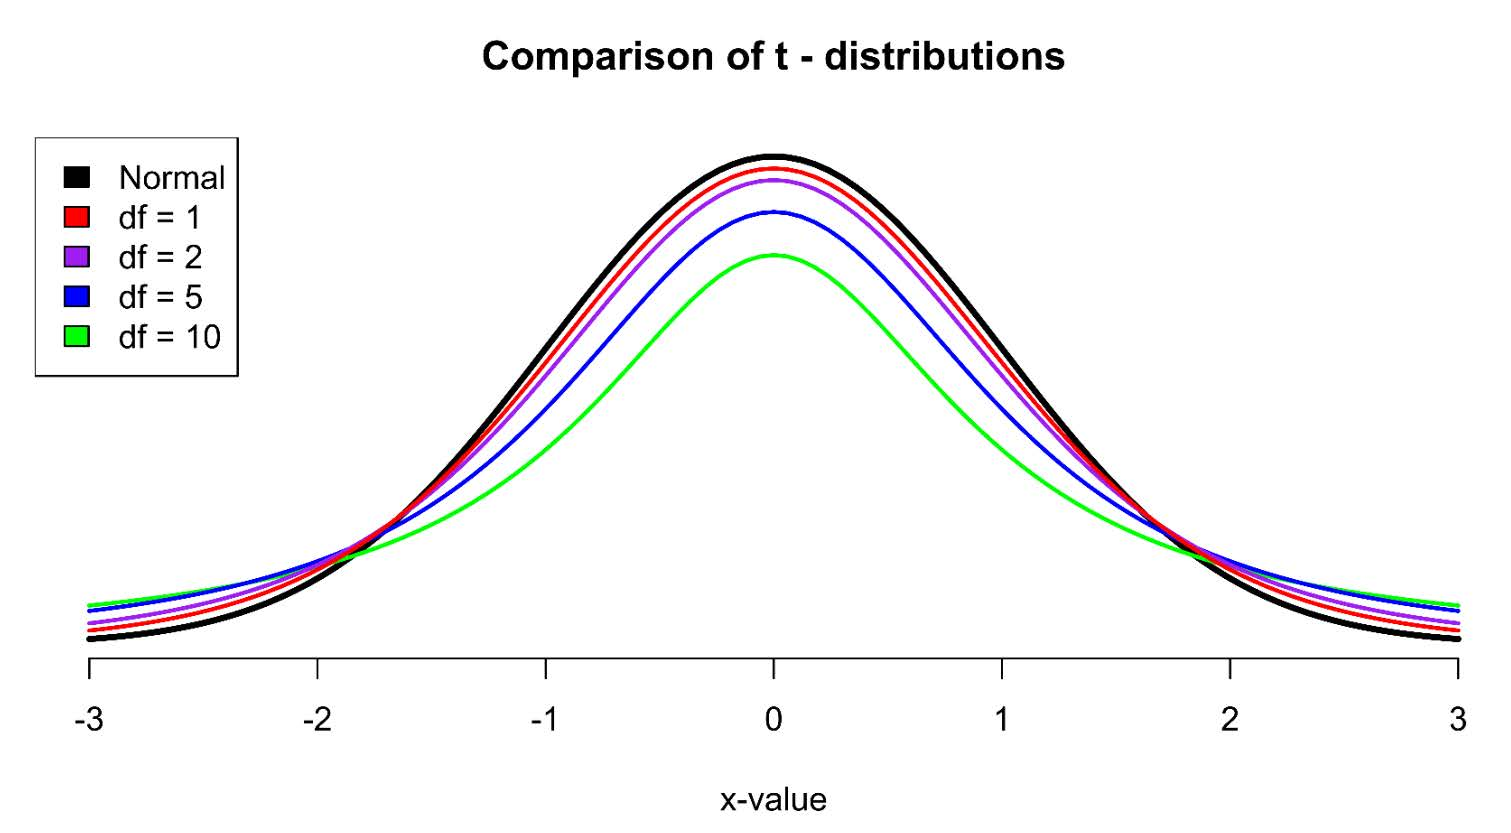
\includegraphics[width=.9\textwidth]{Files/Images/tdistributions.jpg}
\end{center}

Use the following \texttt{R} code to create a figure of the \concept{t-distribution} with $df = 3$. \\

\codeblock{curve(dnorm(x, mean = 0, sd = 1), from = -3, to = 3, ylab = \textquotesingle Density\textquotesingle)\\
curve(dt(x, df = 3), from = -3, to = 3, add = TRUE, col = \textquotesingle red\textquotesingle)
}

\question{
    4.3 d
}{
    Which line represents the \concept{normal distribution} in the figure that was drawn? And which line represents the \concept{t-distribution}? Can you explain what the difference between the two distributions is in terms of their shape? What happens when you increase the \concept{degrees of freedom} (\rcode{df}) in the \rcode{dt()} function?
}

\twolineanswerbox{4.3d}

\question{
    4.3 e
}{
    Calculate the \concept{degrees of freedom} and the \concept{t-value} for the \concept{correlation coefficient} between \rcode{Distance} and \rocde{AvgVisits}.
}

\hint{Hint 4.7: You can find the formula for the \concept{degrees of freedom} and the \concept{t-value} of a \concept{correlation} in the formula sheet.}

\clearpage % Page break

\rcodeanswertiny{4.3e}

\emptyanswerbox{
    4.3e
}{
    $df$: \shortanswerline \hspace*{3cm} $t_{xy}$: \shortanswerline
}

\question{
    4.3 f
}{
    Where do you find the \concept{t-value} that you calculated in assignment 4.3e in the output of the \rcode{cor.test()} function from assignment 4.3c?
}

\onelineanswerbox{4.3f}

\question{
    4.3 g
}{
    What is the \concept{p-value} for this hypothesis test? Interpret this \concept{p-value} with respect to the confidence used and give a conclusion on the hypotheses. Include the following elements:
    \begin{itemize}
        \item[$\square$] Discuss what the \concept{p-value} is for this test.
    \item[$\square$] Discuss whether $H_0$ is rejected or not.
    \item[$\square$] Describe what this tells us about $\rho_{xy}$.  
    \item[$\square$] Describe what type of error is relevant \textit{(type-I or type-II)}.
\end{itemize}
}

\sixlineanswerbox{4.3g}

\clearpage % Page break
%%%%%%%%%%%%%%%%%%%%%%%%%%%%%%%%%%%%%%%%%%%%%%%%%%%%%%%%%%%%%%%%%%%%%%%%%%%
% Assignment 4.4: Testing hypotheses using linear regression in R
%%%%%%%%%%%%%%%%%%%%%%%%%%%%%%%%%%%%%%%%%%%%%%%%%%%%%%%%%%%%%%%%%%%%%%%%%%%

\rassignment{Assignment 4.4: Testing hypotheses using linear regression in R}

A manager from a local supermarket wants to increase the sustainability of her store. Since the supermarket is located in a farm village that has easy access to milk, many milk cartons are not sold, expire, and have to be thrown away. From common sense, the manager suspects that decreasing the price of milk will result in more sales, and thus fewer milk cartons that get thrown away. In order to increase her sustainability through this method, the manager sets out to find out if a decrease in the price per carton of milk will result in fewer milk cartons thrown away on an average day. She also wants to predict her decrease in waste when she lowers the price of a milk carton by 30 cents. \\

The manager goes to the company headquarters and asks the prices of milk (they vary) in every branch of the supermarket chain in the Netherlands. She also asks the average number of milk cartons thrown away per day of each branch. \\

For this assignment, you need the data file \dataset{nationalSupermarket.csv}, which contains the full \concept{population} of 200 stores of the supermarket chain in the Netherlands. \\

\question{
    4.4 a
}{
    Use the \rcode{read.csv()} function (and \rcode{setwd()} function if you prefer) to import the data set into a data frame called \rcode{dataset7}.
}

\rcodeanswertiny{4.4a}

\question{
    4.4 b
}{
    Create a scatter plot of the data. Put the price per milk carton (\rcode{Price}) on the \textit{x-axis} and the average number of milk cartons that was thrown away (\rcode{AvgWasted}) on the \textit{y-axis}.
}

\rcodeanswersmall{4.4b}

The \rcode{lm()} function is used to fit a linear model (linear regression) in \texttt{R}. It requires that you specify a \rcode{formula} that tells the function what the \concept{regression equation} is. If you want to fit a \concept{model} where you predict an outcome variable \rcode{Y} on the basis of one predictor variable \rcode{X}, the formula is as follows: \\

\begin{center}
    \textbf{Formula on paper: }$Y = \beta_0 + \beta_1 \times X$ 
    \hspace*{2cm}
    \textbf{Formula in R: }\rcode{Y {\raise.17ex\hbox{$\scriptstyle\sim$}} 1 + X}
\end{center}

\question{
    4.4 c
}{
    Write down the \concept{regression equation} for a linear model where you predict the average number of thrown away milk cartons per day (\rcode{AvgWasted}) on the basis of the price per milk carton (\rcode{Price}). 
}

\emptyanswerbox{
    4.4c
}{
    AvgWasted = \longanswerline
}

\clearpage % Page break

A linear \concept{model} with these variables can be fitted in \texttt{R} by calling the \rcode{lm()} function with the \rcode{formula} and the \rcode{dataset} (see the \texttt{R} code below). The variables \rcode{X} and \rcode{Y} should correspond to the names of the corresponding variables in your \rcode{dataset}. \\

\codeblock{lm(formula = Y {\raise.17ex\hbox{$\scriptstyle\sim$}} 1 + X, data = dataset)}

\question{
    4.4 d
}{
    Fit a linear \concept{model} where you use the data in \rcode{dataset7} to predict the average number of thrown away milk cartons per day (\rcode{AvgWasted}) on the basis of the price per milk carton (\rcode{Price}). Store this \concept{model} in an object called \rcode{lmfit}.
}

\rcodeanswertiny{4.4d}

Now run the following code in \texttt{R}: \\

\codeblock{summary(lmfit)}

\question{
    4.4 e
}{
    Use the summary to find out the $\beta_0$ and $\beat_1$ parameters and write them down in the \concept{regression equation} below.
}

\emptyanswerbox{
    4.4e
}{
    AvgWasted = $\beta_0$ (\rule{1cm}{0.4pt}) + $\beta_1$ (\rule{1cm}{0.4pt}) $\times$ Price
}

\question{
    4.4 f
}{
    Using the \rcode{abline()} function, paste the \concept{regression equation} line into your scatter plot from assignment 4.4b.
}

\rcodeanswertiny{4.4f}

\question{
    4.4 g
}{
    What is the $R^2$ of the \rcode{lmfit} regression \concept{model}? What is the interpretation of this value?
}

\emptyanswerbox{
    4.4g
}{
    $R^2 = $\shortanswerline    
    \answerskip
    Interpretation:
    \answerskip
    \rule{\textwidth}{0.4pt}
    \answerskip
    \rule{\textwidth}{0.4pt}
}

\clearpage % Page break

From the regression line, the manager observes that there is indeed a positive \concept{relationship} between the price of a carton of milk and the average number of milk cartons thrown away per day. To be sure she wants to test the hypothesis that, with 95\% confidence, the price of milk is a good predictor of the average number of milk cartons that are thrown away per day, and that this \concept{relationship} is truly positive. \\

\question{
    4.4 h
}{
    Formulate the \concept{null hypothesis} $H_0$ and the \concept{alternative hypothesis} $H_1$ for the manager’s test of the population coefficient $\beta_1$ for the price of a carton of milk.  
}

\hypothesesbox{4.4h}

\question{
    4.4 i
}{
    Use the \rcode{summary} in \texttt{R} to draw the conclusion for the manager. Include the following four elements:
        \begin{itemize}
        \item[$\square$] Discuss what the \concept{p-value} is for this test.
        \item[$\square$] Discuss whether $H_0$ is rejected or not.
        \item[$\square$] Describe what this tells us about $\beta_1$.
        \item[$\square$] Describe what type of error is relevant \textit{(type-I or type-II)}.
    \end{itemize}
}

\sixlineanswerbox{4.4i}

\clearpage % Page break
%%%%%%%%%%%%%%%%%%%%%%%%%%%%%%%%%%%%%%%%%%%%%%%%%%%%%%%%%%%%%%%%%%%%%%%%%%%
% Assignment 4.5: Making predictions using linear regression in R
%%%%%%%%%%%%%%%%%%%%%%%%%%%%%%%%%%%%%%%%%%%%%%%%%%%%%%%%%%%%%%%%%%%%%%%%%%%

\rassignment{Assignment 4.5: Making predictions using linear regression in R}

The manager now wants to know what will happen to the number of milk cartons that she has to throw away when she lowers the price of a milk carton by 30 cents, from \$1.00 to \$0.70. Currently, the supermarket throws away 4 cartons of milk each day. \\

\question{
    4.5 a
}{
    Create a new data frame that has only one column that includes the new value for the price of milk (the column has to be named exactly the same as in \rcode{dataset7}).
}

\rcodeanswersmall{4.5a}

The \rcode{predict()} function can be used to predict new data according to a \concept{linear model}. \\

\question{
    4.5 b
}{
    Use the \rcode{predict()} function to predict the number of milk cartons that the supermarket will have to throw away when the \rcode{Price} is \$0.70.
}

\rcodeanswertiny{4.5b}

\emptyanswerbox{
    4.5b
}{
    Predicted value: \shortanswerline
}

\question{
    4.5 c
}{
    Confirm this estimate by writing out the regression equation of the \concept{linear model} from assignment 4.4e and filling in the new value of the price of milk. 
}

\emptyanswerbox{
    4.5c
}{
    Predicted value: \mediumanswerline
}

The \rcode{predict()} function can also be used to construct a \concept{confidence interval} for the predicted number of cartons thrown away by using \rcode{interval = \textquotesingle prediction\textquotesingle}. \\

\clearpage % Page break

\question{
    4.5 d
}{
    Create a 90\% \concept{confidence interval} for the predicted number of milk cartons thrown away. 
}

\rcodeanswertiny{4.5d}

\question{
    4.5 e
}{
    When the manager lowers her price from \$1.00 to \$0.70, will the supermarket throw away fewer cartons of milk? Incorporate the 90\% \concept{confidence interval} for the predicted value in your answer.
}

\emptyanswerbox{
    4.5e
}{
    The supermarket \textbf{will} / \textbf{will not} throw away fewer cartons of milk.
    \answerskip
    Explanation:
    \answerskip
    \rule{\textwidth}{0.4pt}
    \answerbreak
    \rule{\textwidth}{0.4pt}
}

\clearpage % Page break  
\clearpage
\addtocontents{toc}{\protect\vspace{10pt}}
\section{Chapter 5: Comparing one or two means}

\learningobjectives{
    \item Hypothesis testing by hand using the z- and t-score
    \item Generating and interpreting z-scores and t-scores
    \item Independent two-sample t-test by hand and in R
    \item Dependent two-sample t-test in R
}

% To add an assignment to the chapter, create a file in the folder "Assignments" and insert the link below

%%%%%%%%%%%%%%%%%%%%%%%%%%%%%%%%%%%%%%%%%%%%%%%%%%%%%%%%%%%%%%%%%%%%%%%%%%%
% Assignment 5.1: Hypothesis testing by hand using the z- and t-score
%%%%%%%%%%%%%%%%%%%%%%%%%%%%%%%%%%%%%%%%%%%%%%%%%%%%%%%%%%%%%%%%%%%%%%%%%%%

\handassignment{Assignment 5.1: Hypothesis testing by hand using the z- and t-score}

The maximum allowed amount of PFAS chemicals in soil is 0.9 microgram per kg of dry soil. In a regular soil check, researchers take 49 soil \concept{samples} in a town near a plastic factory and find a \concept{mean} PFAS level of 0.918 microgram/kg with a \concept{standard deviation} of 0.071. They want to show with 95\% confidence that the PFAS levels in the town are significantly above the norm. \\

\question{
    5.1 a
}{
    Write down the relevant information from this case.
}

\twolineanswerbox{5.1a}

\question{
    5.1 b
}{
    Write down the \concept{null hypothesis} $H_0$ and the \concept{alternative hypothesis} $H_1$ for the researchers’ test of the \concept{mean} PFAS level against the norm.
}

\hypothesesbox{5.1b}

The \concept{critical z-value} for a one-sided 95\% confidence interval is equal to 1.645 (see also Table 1 on page~\pageref{table1}) \\

\clearpage % Page break

\question{
    5.1 c
}{
    Calculate the \concept{lower bound} of the one-sided \concept{confidence interval} for the PFAS level \concept{population mean} with 95\% confidence.
}

\emptyanswerbox{
    5.1c
}{
    Lower bound: \shortanswerline
    \answerskip
    Calculation:
    \answerskip
    \rule{\textwidth}{0.4pt}
}

\question{
    5.1 d
}{
    Draw the conclusion for the researchers. Include the following four elements:
        \begin{itemize}
    \item[$\square$] Show how $\mu_0$ relates to the \concept{confidence interval.}
    \item[$\square$] Discuss whether $H_0$ is rejected or not.
    \item[$\square$] Describe what this tells us about $\mu$ and $\mu_0$.
    \item[$\square$] Describe what type of error is relevant \textit{(type-I or type-II)}.
\end{itemize}
}

\sixlineanswerbox{5.1d}

\question{
    5.1 e
}{
    Calculate the \concept{z-score} for this situation.
}

\hint{Hint 5.1: You can find the formula for the \concept{z-score} in the formula sheet. Use $\mu_0$ in this formula.}

\emptyanswerbox{
    5.1c
}{
    z-score: \shortanswerline
    \answerskip
    Calculation:
    \answerskip
    \rule{\textwidth}{0.4pt}
}

\clearpage % Page break

\question{
    5.1 f
}{
    Compare the calculated \concept{z-score} with the \concept{critical z-value}. What does this tell you about the \concept{p-value}?
}

\hint{Hint 5.2: Use the absolute value of the calculated \concept{z-score}.}

\twolineanswerbox{5.1f}

\question{
    5.1 g
}{
    Draw the conclusion again, but now using the \concept{z-score}, is it the same? Include the following elements:
    \begin{itemize}
    \item[$\square$] Show how the calculated \concept{z-score} relates to the \concept{critical z-score}.
    \item[$\square$] Discuss whether $H_0$ is rejected or not.
    \item[$\square$] Describe what this tells us about $\mu$ and $\mu_0$.
    \item[$\square$] Describe what type of error is relevant \textit{(type-I or type-II)}.
\end{itemize}
}

\sixlineanswerbox{5.1g}

The researchers want to quickly check another town near the plastic factory, but have less time available. They take 16 \concept{samples} in the second town and find a much higher \concept{mean} PFAS level of 0.930 microgram/kg with a comparable \concept{standard deviation} of 0.070. \\

\question{
    5.1 h
}{
    Calculate the \concept{t-score} for this situation.
}

\hint{Hint 5.3: You can find the formula for the \concept{t-score} in the formula sheet. Use $\mu_0$ in this formula.}

\clearpage % Page break

\emptyanswerbox{
    5.1h
}{
    t-score: \shortanswerline
    \answerskip
    Calculation:
    \answerskip
    \rule{\textwidth}{0.4pt}
}

The \concept{critical t-value} for a one-sided 95\% \concept{confidence interval} with 15 \concept{degrees of freedom} is equal to 1.753.

\question{
    5.1 i
}{
    Draw the conclusion for the researchers using the (absolute) t-score. Include the following elements:
    \begin{itemize}
        \item[$\square$] Show how the calculated \concept{t-score} relates to the \concept{critical t-score}.
    \item[$\square$] Discuss whether $H_0$ is rejected or not.
    \item[$\square$] Describe what this tells us about $\mu$ and $\mu_0$.
    \item[$\square$] Describe what type of error is relevant \textit{(type-I or type-II)}.
\end{itemize}
}

\sixlineanswerbox{5.1i}

\question{
    5.1 j
}{
    Also calculate the \concept{lower bound} of the one-sided \concept{confidence interval} for the PFAS level \concept{population mean} with 95\% confidence.
}

\emptyanswerbox{
    5.1j
}{
    Lower bound: \shortanswerline
    \answerskip
    Calculation:
    \answerskip
    \rule{\textwidth}{0.4pt}
}

\clearpage % Page break

\question{
    5.1 k
}{
    If you would draw the conclusion based on this \concept{lower bound} would you get the same result? Explain why.
}

\emptyanswerbox{
    3.4g
}{
    The conclusion \textbf{would} / \textbf{would not} be the same.
    \answerskip
    Explanation:
    \answerskip
    \rule{\textwidth}{0.4pt}
    \answerbreak
    \rule{\textwidth}{0.4pt}
}

\question{
    5.1 l
}{
    Why is it that even though the second town shows much higher PFAS level in the \concept{sample} (0.930 vs 0.918) $H_0$ cannot be rejected?
}

\twolineanswerbox{5.1l}

\clearpage % Page break
%%%%%%%%%%%%%%%%%%%%%%%%%%%%%%%%%%%%%%%%%%%%%%%%%%%%%%%%%%%%%%%%%%%%%%%%%%%
% Assignment 5.2: Generating and interpreting z-scores and t-scores
%%%%%%%%%%%%%%%%%%%%%%%%%%%%%%%%%%%%%%%%%%%%%%%%%%%%%%%%%%%%%%%%%%%%%%%%%%%

\rassignment{Assignment 5.2: Generating and interpreting z-scores and t-scores}

In assignment 5.1 you have seen that to calculate a 95\% one-sided \concept{confidence interval} for a \concept{sample} with $n \geq 30$ you need to use the correct \concept{z-value}. Now you are going to find out how to get that number from \texttt{R} using the \rcode{qnorm()} function. The \rcode{qnorm()} function returns the \rcode{x}-value for a certain probability for a specified \concept{normal distribution}, if you do not specify the \concept{mean} (\rcode{mean}) and \concept{standard deviation} (\rcode{sd}) arguments it returns the \concept{z-value} for the \concept{standard normal distribution}. \\

Run the following code in R: \\

\codeblock{qnorm(p = 0.95, mean = 0, sd = 1, lower.tail = TRUE)\\
{\color{dataset} \# Or because the standard normal distribution is the default simply use:}\\
qnorm(0.95)
}

\question{
    5.2 a
}{
    Round the number to 3 decimals. Do you recognise this \concept{z-value}?
}

\emptyanswerbox{
    5.2a
}{
    Result: \shortanswerline
    \answerskip
    \rule{\textwidth}{0.4pt}
}

In assignment 5.1 you have also seen that for the 95\% two-sided \concept{confidence interval} for a \concept{sample} with $n \geq 30$ you can use z = 1.960. Now you are going to learn to reproduce that number in \texttt{R}. \\

Run the following code in R: \\

\codeblock{qnorm(p = 0.975)}

\question{
    5.2 b
}{
    Why do you have to use the 97.5 percentile to get the z-value for the 95\% two-sided \concept{confidence interval}?
}

\twolineanswerbox{5.2b}

\clearpage % Page break

Run the following code in R: \\

\codeblock{pnorm(q = 1.645, mean = 0, sd = 1)\\
pnorm(1.960)
}

\question{
    5.2 c
}{
    Based on the results of this \texttt{R} code explain what the \rcode{pnorm()} function does.
}

\twolineanswerbox{5.2c}

In assignment 5.1 it was stated that the \concept{critical t-value} for a one-sided 95\% \concept{confidence interval} with 15 \concept{degrees of freedom} is equal to 1.753. \\

Run the following code in R: \\

\codeblock{qt(p = 0.95, df = 15)}

\question{
    5.2 d
}{
    Based on the results of this \texttt{R} code explain what the \rcode{qt()} function does.
}

\twolineanswerbox{5.2d}

Run the following code in R: \\

\codeblock{pt(q = 1.753, df = 15)}

\question{
    5.2 e
}{
    Based on the results of this \texttt{R} code explain what the \rcode{pt()} function does.
}

\twolineanswerbox{5.2e}

\clearpage % Page break

\begin{center}
    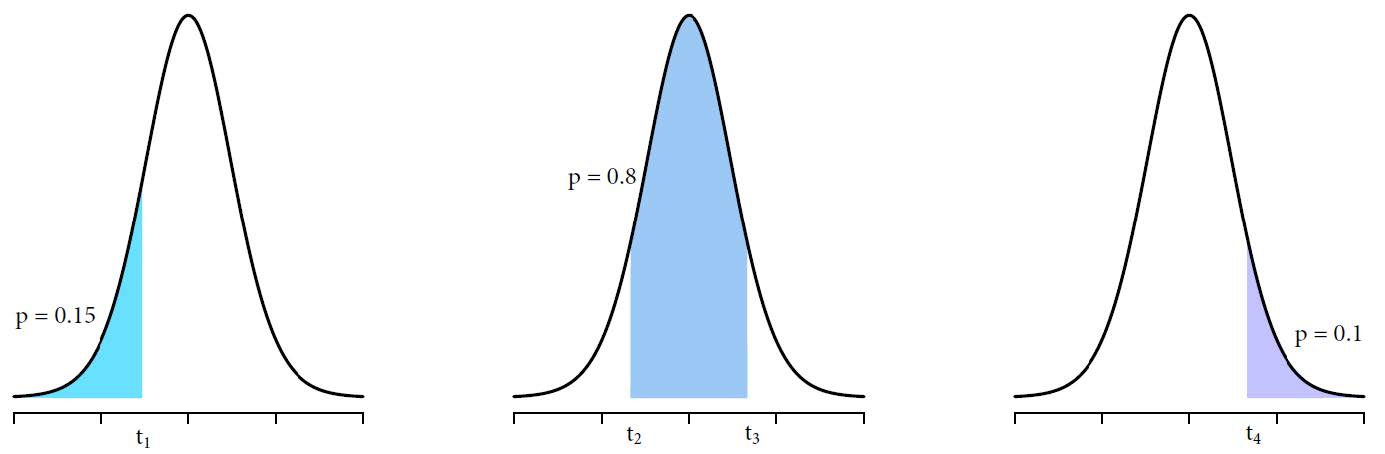
\includegraphics[width=\textwidth]{Files/Images/tdistributions2.jpg}
\end{center}

\question{
    5.2 f
}{
    For the situation where there are 19 \concepts{degrees of freedom}, use the \rcode{qt()} function to get the \concept{t-values} (t$_1$, t$_2$, t$_3$, t$_4$) for the three situations shown in the picture above.
}

\hint{Hint 5.4: For the picture on the right keep in mind that the \rcode{qt()} function by default returns the value for the left tail of the distribution.}

\rcodeanswermedium{5.2f}

\emptyanswerbox{
    5.2f
}{
    t$_1$: \shortanswerline \hspace*{3cm} t$_2$: \shortanswerline
    \answerskip
    t$_3$: \shortanswerline \hspace*{3cm} t$_4$: \shortanswerline
}

\begin{center}
    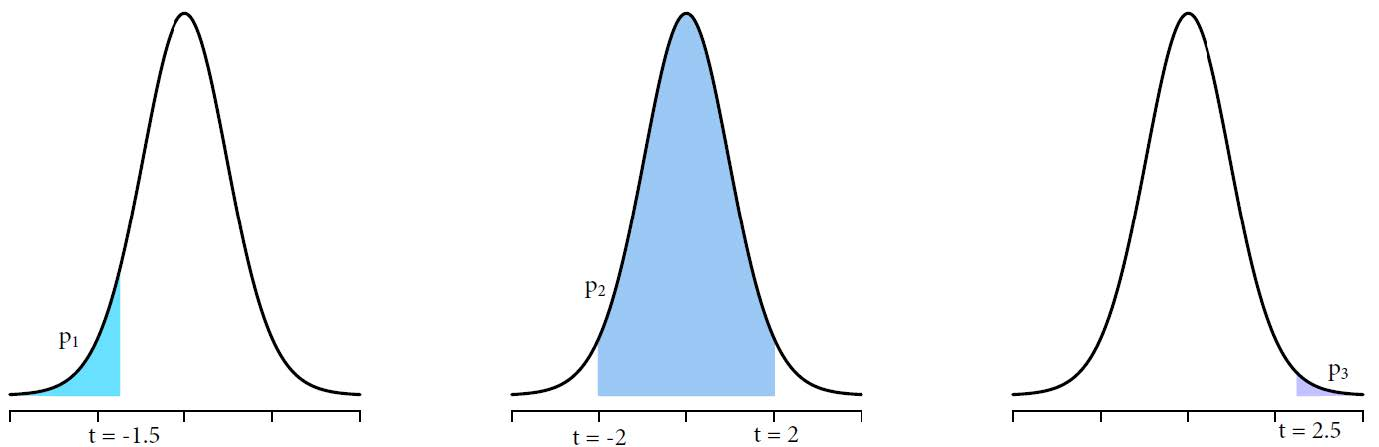
\includegraphics[width=\textwidth]{Files/Images/tdistributions3.jpg}
\end{center}

\clearpage % Page break

\question{
    5.2 g
}{
    For the situation where there are 11 \concept{degrees of freedom}, use the \rcode{pt()} function to get the probabilities p$_1$, p$_2$, and p$_3$ (area under the curve) for the three situations shown in the figures above.
}

\hint{Hint 5.5: For the picture in the middle and the right keep in mind that the \rcode{pt()} function by default uses the left tail and the total area under the curve is 1.}

\rcodeanswermedium{5.2g}

\emptyanswerbox{
    5.2g
}{
    p$_1$: \tinyanswerline \hspace*{2cm} p$_2$: \tinyanswerline \hspace*{2cm} p$_3$: \tinyanswerline
}

When you test a value for a \concept{population mean}, there exist three types of tests: \\

\begin{minipage}[t]{0.33\textwidth}
Two-tailed inequality test: \\
\\
$H_0: \mu = \mu_0$ \\
$H_1: \mu \neq \mu_0$
\end{minipage}
\begin{minipage}[t]{0.33\textwidth}
One-tailed right sided test: \\
\\
$H_0: \mu \leq \mu_0$ \\
$H_1: \mu > \mu_0$
\end{minipage}
\begin{minipage}[t]{0.33\textwidth}
One-tailed left sided test: \\
\\
$H_0: \mu \geq \mu_0$ \\
$H_1: \mu < \mu_0$
\end{minipage}
\vspace*{0.5cm}

\question{
    5.2 h
}{
    Give a critical \concept{t-value} for the three tests described above using a confidence of 98\% and 28 \concept{degrees of freedom}.
}

\hint{Hint 5.6: Use the \rcode{qt()} function in \texttt{R}}.

\rcodeanswermedium{5.2h}

\emptyanswerbox{
    5.2h
}{
    Two-tailed inequality test: \shortanswerline 
    \answerskip
    One-tailed right sided test: \hspace*{-5pt}\shortanswerline 
    \answerskip
    One-tailed left sided test: \shortanswerline 
}

\clearpage % Page break

Three $n = 29$ \concept{samples} were done on three different populations and the \concept{t-score} based on these \concept{samples} was calculated:

\begin{minipage}[t]{0.33\textwidth}
Two-tailed inequality test: \\
\\
$H_0: \mu = 50$ \\
$H_1: \mu \neq \50$ \\
\\
$t = 2.6$
\end{minipage}
\begin{minipage}[t]{0.33\textwidth}
One-tailed right sided test: \\
\\
$H_0: \mu \leq \50$ \\
$H_1: \mu > \50$ \\
\\
$t = -2.3$
\end{minipage}
\begin{minipage}[t]{0.33\textwidth}
One-tailed left sided test: \\
\\
$H_0: \mu \geq \50$ \\
$H_1: \mu < \50$ \\
\\
$t = 1.6$
\end{minipage}
\vspace*{0.5cm}

\question{
    5.2 i
}{
    Using a confidence of 98\%, find out whether the \concept{null hypothesis} $H_0$ is rejected for each of these three cases.
}

\hint{Hint 5.7 : Use the \concept{critical t-values} from the previous assignment and compare these with the sample \concept{t-scores} to draw your conclusion for each of these outcomes.}

\emptyanswerbox{
    5.2i
}{
    Two-tailed inequality test: \hspace*{1.5cm} \textbf{$H_0$ rejected} / \textbf{$H_0$ not rejected}
    \answerbreak
    Explanation: \rule{.75\textwidth}{0.4pt}
    \answerskip
    \answerskip
    One-tailed right sided test: \hspace*{-5pt}\hspace*{1.5cm} \textbf{$H_0$ rejected} / \textbf{$H_0$ not rejected}
    \answerbreak
    Explanation: \rule{.75\textwidth}{0.4pt}
    \answerskip
    \answerskip
    One-tailed left sided test: \hspace*{1.5cm} \textbf{$H_0$ rejected} / \textbf{$H_0$ not rejected}
    \answerbreak
    Explanation: \rule{.75\textwidth}{0.4pt}    
}

\clearpage % Page break
%%%%%%%%%%%%%%%%%%%%%%%%%%%%%%%%%%%%%%%%%%%%%%%%%%%%%%%%%%%%%%%%%%%%%%%%%%%
% Assignment 5.3: Independent two-sample t-test by hand and in R
%%%%%%%%%%%%%%%%%%%%%%%%%%%%%%%%%%%%%%%%%%%%%%%%%%%%%%%%%%%%%%%%%%%%%%%%%%%

\handassignment{Assignment 5.3: Independent two-sample t-test by hand and in R}

To test the effect of caffeine on the respiratory exchange ratio (RER), 9 men get caffeine and 9 different men get a placebo, their RER is measured while doing sports\footnote{These data are taken from \url{http://learntech.uwe.ac.uk/da/Default.aspx?pageid=1438}}: \\
\vspace*{0.5cm}
\begin{center}
\begin{tabular}{c|ccc}
RER measurement & $n$ & Mean ($\bar{x}$) & Standard deviation ($s_x$) \tstrut\bstrut\\
\hline
Caffeine & 9 & 94.22 & 5.61 \tstrut\bstrut\\
Placebo & 9 & 100.56 & 7.70 \tstrut\bstrut\\
\end{tabular}
\end{center}
\vspace*{0.5cm}

Researchers want to use this experiment to show with 95\% confidence that caffeine reduces the RER in men. They are going to evaluate the results by comparing the \concept{mean} RER using a \concept{two-sample t-test}. \\

\question{
    5.3 a
}{
    Why is this test also called an \concept{independent samples t-test}?
}

\twolineanswerbox{5.3a}

\question{
    5.3 a
}{
    Write down the \concept{null hypothesis} $H_0$ and the \concept{alternative hypothesis} $H_1$ for a one-sided test where the researchers want to show that the placebo \concept{mean} RER is higher than the caffeine \concept{mean} RER.
}

\hypothesesbox{5.3b}

In the formula sheet on page~\pageref{formulasheet} you can see that for \concept{independent samples t-tests}:
\vspace*{0.5cm}
\begin{equation*}
    t = \frac{(\bar{x}_1 - \bar{x}_2) - D_0}{\sqrt{s^2_p (\frac{1}{n_1} + \frac{1}{n_2})}}
    \hspace*{3cm}
    s^2_p = \frac{(n_1 - 1) s^2_1 + (n_2 - 1) s^2_2}{n_1 + n_2 - 2}
\end{equation*}
\vspace*{0.5cm}

\question{
    5.3 c
}{
    Using the formula provided calculate the \concept{pooled standard deviation} $s_p$.
}

\clearpage % Page break

\emptyanswerbox{
    5.3c
}{
    $s_p$: \shortanswerline
    \answerskip
    Calculation:
    \answerskip
    \rule{\textwidth}{0.4pt}
}

\question{
    5.3 d
}{
    Using the formula provided calculate the \concept{t-score}.
}

\emptyanswerbox{
    5.3c
}{
    t-score: \shortanswerline
    \answerskip
    Calculation:
    \answerskip
    \rule{\textwidth}{0.4pt}
}

The \concept{critical t-value} for 16 \concept{degrees of freedom} $(n_1 + n_2 - 2)$ for a one-sided test is 1.746. \\

\question{
    5.3 e
}{
    Draw the conclusion for this test. Include the following elements:
        \begin{itemize}
        \item[$\square$] Show how the calculated \concept{t-score} relates to the \concept{critical t-score}.
    \item[$\square$] Discuss whether $H_0$ is rejected or not.
    \item[$\square$] Describe what this tells us about $\mu$ and $\mu_0$.
    \item[$\square$] Describe what type of error is relevant \textit{(type-I or type-II)}.
\end{itemize}
}

\sixlineanswerbox{5.3e}

\clearpage % Page break

\begin{minipage}{0.8\textwidth}
Now you will learn how to do the same independent t-test in \texttt{R}. \\

Run the following code in \texttt{R}: \\
\end{minipage}%
\hfill%
\begin{minipage}{0.1\textwidth}

\includegraphics[width=\linewidth]{Files/Images/displaycode.pdf}
\end{minipage}
\vspace*{.1cm}

\codeblock{{\color{dataset}\# These are the values for the RER test data set}\\
placebo <- c(105, 119, 100, 97, 96, 101, 94, 95, 98)\\
caffeine <- c(96, 99, 94, 89, 96, 93, 88, 105, 88)}

\question{
    5.3 f
}{
    Calculate the \concept{mean} and \concept{standard deviation} for the \rcode{placebo} and \rcode{caffeine} variables, confirm that your results match with the previous assignment.
}

\rcodeanswermedium{5.3f}

\emptyanswerbox{
    5.3f
}{
    \rcode{placebo} \hspace*{6cm} \rcode{caffeine}
    \answerskip
    Mean: \hspace{90pt}\tinyanswerline \hspace*{2cm}Mean: \hspace{80pt}\tinyanswerline
    \answerskip
    Standard deviation: \tinyanswerline \hspace*{1.95cm}Standard deviation: \tinyanswerline
}

Run the following code in \texttt{R}: \\

\codeblock{t.test(x = placebo, y = caffeine, alternative = \textquotesingle greater\textquotesingle, mu = 0, \\
       \hspace*{40pt}paired = FALSE, var.equal = TRUE, conf.level = 0.95)}

\question{
    5.3 g
}{
    Interpret the \texttt{R} code above and check if the results match your conclusion for assignment 5.3e.
}

\twolineanswerbox{5.3g}

The \concept{t-test} assumes equal \concept{variances}. In this case the \concept{standard deviations} are actually a bit different. \\

\clearpage % Page break

\question{
    5.3 h
}{
    Change the \rcode{var.equal} argument in the \texttt{R} code above to do a \concept{Welch t-test} to account for unequal \concept{variances}. Check whether the results differ.
}

\rcodeanswertiny{5.3h}

\twolineanswerbox{5.3h}

\question{
    5.3 i
}{
    How can you check if you need to do a \concept{Welch t-test} instead of a normal \concept{t-test}?
}

\twolineanswerbox{5.3i}

\clearpage % Page break
%%%%%%%%%%%%%%%%%%%%%%%%%%%%%%%%%%%%%%%%%%%%%%%%%%%%%%%%%%%%%%%%%%%%%%%%%%%
% Assignment 5.4: Dependent two-sample t-test in R
%%%%%%%%%%%%%%%%%%%%%%%%%%%%%%%%%%%%%%%%%%%%%%%%%%%%%%%%%%%%%%%%%%%%%%%%%%%

\rassignment{Assignment 5.4: Dependent two-sample t-test in R}

To test for a difference in blood pressure depending on their position, 12 people’s blood pressure was measured twice, first standing up and then lying down. Researchers want to use this experiment to show with 92.5\% confidence that the blood pressure lying down is significantly higher than standing up. They are going to evaluate the results by comparing the \concept{mean} using a \concept{two-sample t-test}. \\

\question{
    5.4 a
}{
    Why is this a dependent (also called paired) \concept{t-test}?
}

\twolineanswerbox{5.4a}

Run the following code in \texttt{R}: \\

\codeblock{{\color{dataset}\# These are the values for the blood pressure data set} \\
standing <- c(132, 146, 135, 141, 139, 162, 128, 137, 145, 151, 131, 
              143) \\
lying <- c(136, 145, 140, 147, 142, 160, 137, 136, 149, 158, 120, 150)}

\question{
    5.4 b
}{
    Calculate the \concept{mean} of the \rcode{standing} and \rcode{lying} data sets, also calculate the differences and the \concept{mean} of the differences.
}

\rcodeanswersmall{5.4b}

\emptyanswerbox{
    5.4b
}{
    Mean standing: \quad \shortanswerline
    \answerskip
    Mean lying: \qquad \quad \shortanswerline
    \answerskip
    Mean difference: \shortanswerline
}

\clearpage % Page break

\question{
    5.4 c
}{
    Write down the \concept{null hypothesis} $H_0$ and \concept{alternative hypothesis} $H_1$ for a one-sided test where the researchers want to show with 92.5\% confidence that the \concept{mean} blood pressure is higher lying down than standing up.
}

\hypothesesbox{5.4c}

Run the following code in \texttt{R}: \\

\codeblock{t.test(x = standing, y = lying, alternative = \textquotesingle greater\textquotesingle, mu = 0 , \\
       \hspace*{40pt}paired = TRUE, conf.level = 0.925)}
       
\question{
    5.4 d
}{
    Check the results of this test. The outcome is a bit strange, can you explain what is wrong here?
}

\onelineanswerbox{5.4d}

\question{
    5.4 e
}{
    Fix the \texttt{R} code to do a correct test and draw the correct (four part) conclusion.
}

\rcodeanswersmall{5.4e}
\sixlineanswerbox{5.4e}

\clearpage % Page break  
\clearpage
\addtocontents{toc}{\protect\vspace{10pt}}
\section{Chapter 6: Comparing more than two means}

\learningobjectives{
    \item Implementing a t-test as a regression in R
    \item Performing an ANOVA in R
    \item Implementing an ANOVA as a regression in R
    \item Introducing a covariate in ANCOVA in R
}

% To add an assignment to the chapter, create a file in the folder "Assignments" and insert the link below

%%%%%%%%%%%%%%%%%%%%%%%%%%%%%%%%%%%%%%%%%%%%%%%%%%%%%%%%%%%%%%%%%%%%%%%%%%%
% Assignment 6.1: Implementing a t-test as a regression in R
%%%%%%%%%%%%%%%%%%%%%%%%%%%%%%%%%%%%%%%%%%%%%%%%%%%%%%%%%%%%%%%%%%%%%%%%%%%

\rassignment{Assignment 6.1: Implementing a t-test as a regression in R}

Many of the statistical tests that we have seen are actually equivalent to a specific form of \concept{linear regression}. To understand how a \concept{t-test} can be implemented as a \concept{linear regression}, let’s look at an example. Suppose you work in advertising and show four groups of people an advertisement, where the only difference is in the color/position of the eyes of the model (blue eyes, brown eyes, green eyes, or downward-looking eyes), and you ask them how they rate your brand after seeing this advertisement. For this assignment, we will use the \dataset{eyeColor.csv} data file that contains 222 participants’ ratings for one of the four groups. As a first question, you want to assess whether there is a difference in the ratings if the model shown in the advertisement has blue eyes rather than brown eyes. \\

\question{
    6.1 a
}{
    Read in the file \dataset{eyeColor.csv} and store the data in an object called \rcode{dataset8}.
}

\rcodeanswertiny{6.1a}

Note that this data set contains all four groups (\rcode{Blue}, \rcode{Brown}, \rcode{Green}, \rcode{Down}). Run the following \texttt{R} code to isolate the scores of the groups that were shown advertisements with \rcode{Blue} and \rcode{Brown} eyes and store them in the new \rcode{ttestData} object. \\

\codeblock{ttestData  <- subset(dataset8,\\ 
                     \hspace*{110pt}dataset8\$Group == \textquotesingle Blue\textquotesingle | \\
                     \hspace*{110pt}dataset8\$Group == \textquotesingle Brown\textquotesingle)}

\question{
    6.1 b
}{
    Write down the \concept{null hypothesis} $H_0$ and \concept{alternative hypothesis} $H_1$ for testing whether the \concept{mean} score of the group that was shown \rcode{Blue} eyes is equal to the \concept{mean} score of the group that was shown \rcode{Brown} eyes. Remember that these are independent \concept{samples}.
}

\hypothesesbox{6.1b}

\question{
    6.1 c
}{
    Use the \rcode{t.test()} function to test the equality of the two means.
}

\hint{Hint 6.1: Make sure to specify \rcode{var.equal = TRUE} to perform a \concept{two-sample t-test} instead of the non-parametric \concept{Welch’s t-test}.}

\rcodeanswertiny{6.1c}

\question{
    6.1 d
}{
    What is your conclusion on the basis of these results? Include the following elements:
        \begin{itemize}
        \item[$\square$] Discuss what the \concept{p-value} is for this test.
    \item[$\square$] Discuss whether $H_0$ is rejected or not.
    \item[$\square$] Describe what this tells us about $\mu_{Blue}$ and $\mu_{Brown}$.  
    \item[$\square$] Describe what type of error is relevant \textit{(type-I or type-II)}.
\end{itemize}
}

\sixlineanswerbox{6.1d}

Now, instead of using the \rcode{t.test()} function to test the equality of the two \concept{means}, you can test the equality of the two \concept{means} using a \concept{regression model}. Therefore, you need to add a variable to our data that says whether a participant saw one of the two groups (e.g., only the people that were shown \rcode{Brown} eyed models). \\

Run the following code in R: \\

\codeblock{dummyBrown <- as.numeric(ttestData\$Group == \textquotesingle Brown\textquotesingle)\\
ttestData <- cbind(ttestData, dummyBrown)}

\clearpage % Page break

\question{
    6.1 e
}{
    What are the contents of \rcode{dummyBrown}? What do we call this kind of variable?
}

\twolineanswerbox{6.1e}

\question{
    6.1 f
}{
    Create a \concept{linear model} in \texttt{R} where you predict the (outcome) variable \rcode{Score} using only the (predictor) variable \rcode{dummyBrown}. Store the fitted model in an object called \rcode{ttestreg}.
}

\rcodeanswersmall{6.1f}

\question{
    6.1 g
}{
    Use the \rcode{summary()} function to inspect the results of the \rcode{ttestreg} model. How does this output correspond to the \concept{t-test} that you performed in assignment 6.1c? Where do you find the \concept{p-value} that you calculated using the \rcode{t.test()} function?
}

\rcodeanswersmall{6.1g}

\twolineanswerbox{6.1g}

\clearpage % Page break
%%%%%%%%%%%%%%%%%%%%%%%%%%%%%%%%%%%%%%%%%%%%%%%%%%%%%%%%%%%%%%%%%%%%%%%%%%%
% Assignment 6.2: Performing an ANOVA in R
%%%%%%%%%%%%%%%%%%%%%%%%%%%%%%%%%%%%%%%%%%%%%%%%%%%%%%%%%%%%%%%%%%%%%%%%%%%

\rassignment{Assignment 6.2: Performing an ANOVA in R}

Now let’s extend the analysis from assignment 6.1 by comparing all four groups (\rcode{Blue}, \rcode{Brown}, \rcode{Green}, \rcode{Down}) instead of only the \rcode{Blue} and \rcode{Brown} groups. When you are testing more than two \concept{means}, you can use an \concept{ANOVA} test (a specific form of regression). Since you want to compare all four groups, you can leave the \rcode{ttestData} from the previous assignment and focus on the data in \rcode{dataset8}. Remember that you are interested in testing the effect of the model’s eye color on the rating of your brand. \\

\question{
    6.2 a
}{
    Write down the \concept{null hypothesis} $H_0$ and the \concept{alternative hypothesis} $H_1$ for testing whether the \concept{mea}n score of the four groups (\rcode{Blue}, \rcode{Brown}, \rcode{Green}, \rcode{Down}) are equal.
}

\hypothesesbox{6.2a}

The \concept{ANOVA} uses the \concept{F-distribution} to test for a significant difference between all four \concept{means}. Using the (two types of) \concept{degrees of freedom} of this \concept{F-distribution}, you can calculate the \concept{critical F-value} that is required to reject the \concept{null hypothesis} that the \concept{means} of the four groups are equal. Table 5 on page~\pageref{table5} contains the \concept{critical F-values} for a confidence of 95\%.
\vspace*{.5cm}
\begin{center}
    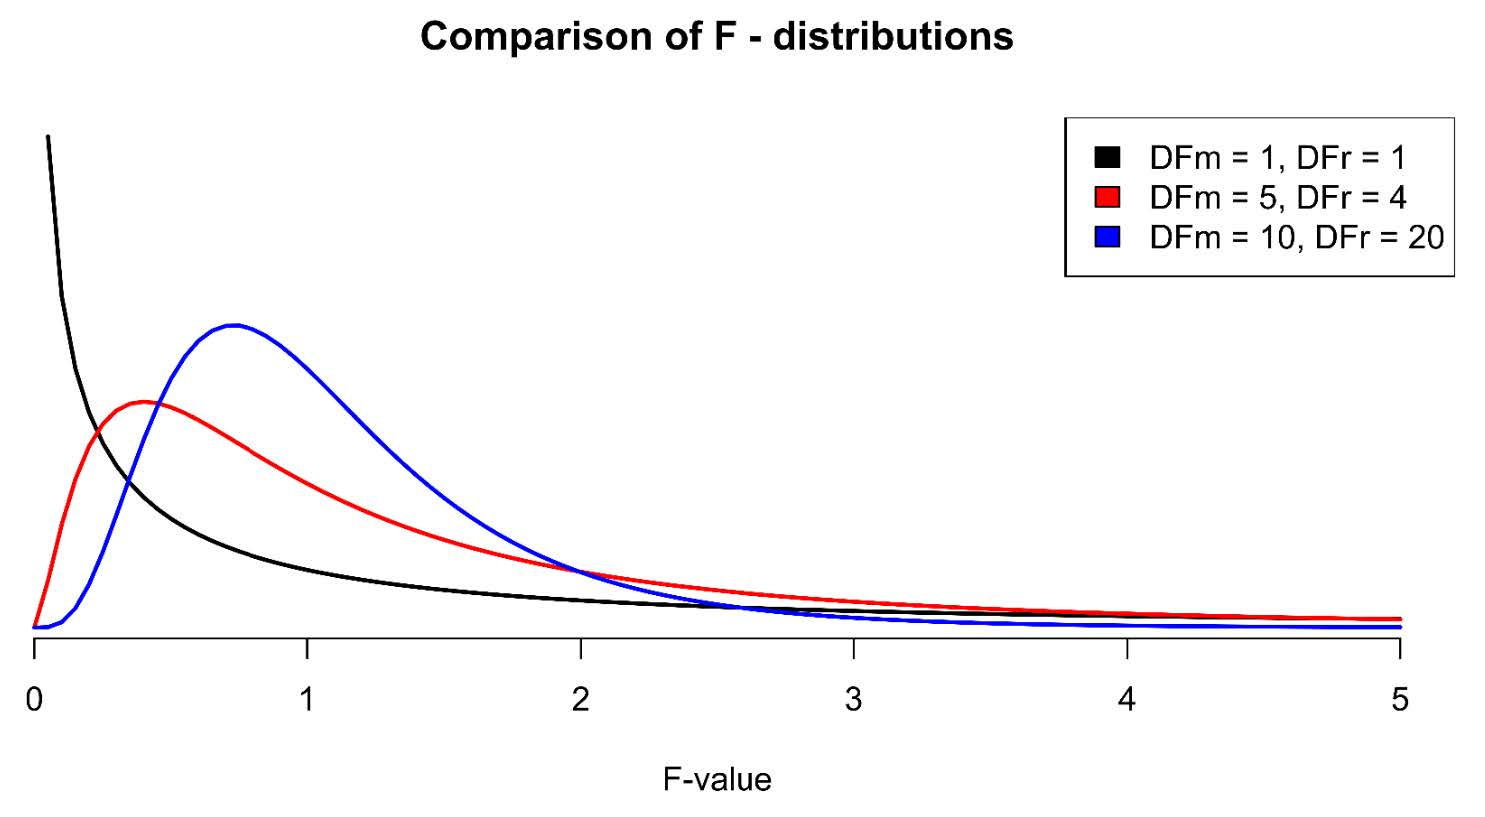
\includegraphics[width=.9\textwidth]{Files/Images/fdistributions.jpg}
\end{center}

\clearpage % Page break

\question{
    6.2 b
}{
    Calculate the \concept{degrees of freedom} $df_M$ and $df_R$ of the \concept{F-distribution} for the data in \rcode{dataset8}.
}

\hint{Hint 6.2: You can find the formulas for $df_M$ and $df_R$ in the formula sheet.}

\emptyanswerbox{
    6.2b
}{
    $df_M$: \shortanswerline \hspace*{3cm} $df_R$: \shortanswerline
}

\question{
    6.2 c
}{
    Using the \rcode{qf()} function, calculate the \concept{critical F-value} that is required to reject the \concept{null hypothesis} $H_0$ for these data with 95\% confidence.
}

\rcodeanswertiny{6.2c}

\emptyanswerbox{
    6.2c
}{
    Critical F-value: \shortanswerline
}

The \rcode{aov()} function in \texttt{R} is a wrapper for the \rcode{lm()} function. The difference between these two functions is that the \rcode{lm()} function can only handle \concept{categorical} predictors with two levels (e.g., a \concept{dummy variable}). The \rcode{aov()} function can handle \concept{categorical} predictor variables with more than two levels, since it automatically rewrites the \rcode{formula} to include the \concept{dummy variables}. \\ 

\question{
    6.2 d
}{
    Use the \rcode{aov()} function to perform an \concept{ANOVA} with the dependent (outcome) variable \rcode{Score} and the independent (predictor) variable \rcode{Group} and store the result in an object named \rcode{anovaResult}.
}

\hint{Hint 6.3: You can check more information on the \rcode{aov()} function with \rcode{?aov}.}

\rcodeanswersmall{6.2d}

\clearpage % Page break

\question{
    6.2 e
}{
    Use the \rcode{summary()} function to inspect the results of the \concept{ANOVA} in \rcode{anovaResult}. What is the \concept{F-value} that is calculated from the \concept{sample}? What is the \concept{p-value} calculated from the \concept{sample}?
}

\rcodeanswertiny{6.2e}

\emptyanswerbox{
    6.2e
}{
    F-value: \shortanswerline \hspace*{3cm} p-value: \shortanswerline
}

\question{
    6.2 f
}{
    What is your conclusion on the basis of these results? Include the following elements:
        \begin{itemize}
        \item[$\square$] Discuss what the \concept{p-value} is for this test.
    \item[$\square$] Discuss whether $H_0$ is rejected or not.
    \item[$\square$] Describe what this tells us about $\mu_{Blue}$, $\mu_{Brown}$, $\mu_{Green}$, and $\mu_{Down}$.  
    \item[$\square$] Describe what type of error is relevant \textit{(type-I or type-II)}.
\end{itemize}
}

\sixlineanswerbox{6.2f}

\clearpage % Page break
%%%%%%%%%%%%%%%%%%%%%%%%%%%%%%%%%%%%%%%%%%%%%%%%%%%%%%%%%%%%%%%%%%%%%%%%%%%
% Assignment 6.3: Implementing an ANOVA as a regression in R
%%%%%%%%%%%%%%%%%%%%%%%%%%%%%%%%%%%%%%%%%%%%%%%%%%%%%%%%%%%%%%%%%%%%%%%%%%%

\rassignment{Assignment 6.3: Implementing an ANOVA as a regression in R}

Now that you have seen the results of the \concept{ANOVA}, let’s try to replicate these by implementing the same \concept{ANOVA} as a \concept{linear regression}. Remember that this is exactly what you did for the \concept{t-test} in assignment 6.1 by adding one \concept{dummy variable} to your model that isolated the \rcode{Brown} group. For the \concept{ANOVA}, you are going to have three \concept{dummy variables} in your model, one that represents  \rcode{Brown} eyes, one that represents \rcode{Blue} eyes, and one that represents \rcode{Green} eyes. You first have to add these dummy variables to your data set. \\

Run the following code in \texttt{R} that adds a \concept{dummy variable} for \rcode{Brown} eyes to the data set: \\

\codeblock{dummyBrown <- as.numeric(dataset8\$Group == \textquotesingle Brown\textquotesingle) \\
dataset8   <- cbind(dataset8, dummyBrown)}

\question{
    6.3 a
}{
    Add two more \concept{dummy variables} to the data in \rcode{dataset8}, one for \rcode{Blue} eyes and one for \rcode{Green} eyes. Name these variables \rcode{dummyBlue} and \rcode{dummyGreen}.
}

\rcodeanswermedium{6.3a}

\question{
    6.3 b
}{
    Create a \concept{linear model} in \texttt{R} where you predict the (outcome) variable \rcode{Score} using the (predictor) variables \rcode{dummyBrown}, \rcode{dummyGreen}, and \rcode{dummyBlue}. Store the fitted \concept{linear model} in an object called \rcode{anovaReg}.
}

\rcodeanswersmall{6.3b}

\question{
    6.3 c
}{
    Use the \rcode{summary()} function to inspect the results of the \concept{linear model} stored in \rcode{anovaReg}. What is the \concept{F-value} of the model? What is the \concept{p-value} of this model?
}

\rcodeanswertiny{6.3c}

\emptyanswerbox{
    6.3c
}{
    F-value: \shortanswerline \hspace*{3cm} p-value: \shortanswerline
}

\clearpage % Page break

\question{
    6.3 d
}{
    Do the \concept{F-value} and \concept{p-value} of this \concept{linear model} match those of the \concept{ANOVA} in assignment 6.2?
}

\emptyanswerbox{
    6.3d
}{
    \vspace*{-15pt}
    \begin{center}
        YES / NO
    \end{center}
}

\clearpage % Page break
%%%%%%%%%%%%%%%%%%%%%%%%%%%%%%%%%%%%%%%%%%%%%%%%%%%%%%%%%%%%%%%%%%%%%%%%%%%
% Assignment 6.4: Introducing a covariate in ANCOVA in R
%%%%%%%%%%%%%%%%%%%%%%%%%%%%%%%%%%%%%%%%%%%%%%%%%%%%%%%%%%%%%%%%%%%%%%%%%%%

\rassignment{Assignment 6.4: Introducing a covariate in ANCOVA in R}

There might be other determinants that influence people’s ratings of your brand that you have not captured by varying the eye color in the advertisements. An example of this might be people’s initial rating of your brand. These kinds of variables are called \concept{covariates} and you can incorporate them in our \concept{ANOVA}, very smoothly resulting in an \concept{ANCOVA}. In our scenario, we want to incorporate the \concept{covariate} for the initial score that our raters gave by adding the \rcode{initialScore} variable to our \concept{linear model}. \\

\question{
    6.4 a
}{
    Create a \concept{linear model} in \texttt{R} where you predict the (outcome) variable \rcode{Score} using the (predictor) variables \rcode{dummyBrown}, \rcode{dummyGreen}, \rcode{dummyBlue}, and the variable \rcode{initialScore}. Store the fitted model in an object called \rcode{ancovaReg}.
}

\rcodeanswersmall{6.4a}

\question{
    6.4 b
}{
    Use the \rcode{summary()} function to inspect the results of the \concept{linear model} stored in \rcode{ancovaReg}. What is the \concept{F-value} of the model? What is the \concept{p-value} of this model?
}

\rcodeanswertiny{6.4b}

\emptyanswerbox{
    6.4b
}{
    F-value: \shortanswerline \hspace*{3cm} p-value: \shortanswerline
}

\question{
    6.4 c
}{
    What is your conclusion on the basis of these results? Include the following elements:
        \begin{itemize}
        \item[$\square$] Discuss what the \concept{p-value} is for this test.
    \item[$\square$] Discuss whether $H_0$ is rejected or not.
    \item[$\square$] Describe what this tells us about $\mu_{Blue}$, $\mu_{Brown}$, $\mu_{Green}$, and $\mu_{Down}$, given the covariate.  
    \item[$\square$] Describe what type of error is relevant \textit{(type-I or type-II)}.
\end{itemize}
}

\threelineanswerbox{6.4c}

\clearpage % Page break

\question{
    6.4 d
}{
    Can you tell whether \rcode{initialScore} is a good predictor of the \rcode{Score}? On what value can you base your conclusion?
}

\hint{Hint 6.4: First consider which results you would expect if $\beta_3 \neq 0$.}

\twolineanswerbox{6.4d}

To find out whether adding this \concept{covariate} is an improvement over the \concept{linear model} in assignment 6.3, we can compare the two \concept{linear models} \rcode{anovaReg} (without \rcode{initialScore}) and \rcode{ancovaReg} (with \rcode{initialScore}) with respect to their proportion of \concept{explained variance} (their $R^2$).  \\

\question{
    6.4 e
}{
    What is the (multiple) $R^2$ of the \rcode{anovaReg} \concept{model}? What is the (multiple) $R^2$ of the \rcode{ancovaReg} \concept{model}? Which \concept{model} explains more variation in the outcome variable \rcode{Score}?
}
    
\emptyanswerbox{
    6.4e
}{
    $R^2$ \rcode{anovaReg}: \shortanswerline \hspace*{1cm} $R^2$ \rcode{ancovaReg}: \shortanswerline
    \answerskip
    The \rcode{anovaReg} / \rcode{ancovaReg} regression model explains more variation in the outcome variable score.
}

\question{
    6.4 f
}{
    Interpret the $R^2$ for the best model.
}

\twolineanswerbox{6.4f}

The $R^2$ statistic will always increase when you add more (predictor) variables to our \concept{model}, since you are adding more information. To reliably compare our two \concept{models}, you have to look at a measure that penalizes a \concept{model} for including more (predictor) variables. You can use the \concept{AIC} value for that. The rule of thumb for the \concept{AIC} value is that the \concept{model} with the lower \concept{AIC} value is the preferred model. \\

\clearpage % Page break

\question{
    6.4 g
}{
    Use the \rcode{AIC()} function to calculate the \concept{AIC} value of the \rcode{anovaReg} and the \rcode{ancovaReg} models.
}

\rcodeanswersmall{6.4g}

    
\emptyanswerbox{
    6.4g
}{
    AIC \rcode{anovaReg}: \shortanswerline \hspace*{.5cm} AIC \rcode{ancovaReg}: \shortanswerline
}

\question{
    6.4 h
}{
    What is the preferred model? How can you use the \concept{AIC} statistic to validate you answer in assignment 6.4d?
}

\twolineanswerbox{6.4h}

\clearpage % Page break
%%%%%%%%%%%%%%%%%%%%%%%%%%%%%%%%%%%%%%%%%%%%%%%%%%%%%%%%%%%%%%%%%%%%%%%%%%%
% Assignment 6.5: Using post-hoc tests to find differences in means
%%%%%%%%%%%%%%%%%%%%%%%%%%%%%%%%%%%%%%%%%%%%%%%%%%%%%%%%%%%%%%%%%%%%%%%%%%%

\rassignment{Assignment 6.5: Using post-hoc tests in R to find differences in means}

For this assignment you will have to download the data file \dataset{iowa.RData} from the online resources\footnote{These data are taken from \url{https://data.iowa.gov/State-Government-Finance/State-of-Iowa-Checkbook/cyqb-8ina}.}. \dataset{.RData} files are compressed \texttt{R} objects, and are useful when dealing with very large data sets such as this one. \\

The \dataset{iowa.RData} file contains payment transactions recorded in the State of Iowa’s central accounting system for the Executive Branch and is real data. \\

\question{
    6.5 a
}{
    Load the \dataset{iowa.RData} data file into the environment using the \rcode{load()} function. 
}

\rcodeanswertiny{6.5a}

The data set is now stored in object called \rcode{iowa}. \\

\question{
    6.5 b
}{
    Give a short description of the data in \rcode{iowa}.
}

\hint{Hint 6.5: Search the internet for the source of these data to find out what the columns represent.}

\threelineanswerbox{6.5b}

\question{
    6.5 c
}{
    How many rows and columns does the \rcode{iowa} data set have?
}

\emptyanswerbox{
    6.5c
}{
    Rows: \shortanswerline \hspace*{3cm} Columns: \shortanswerline
}

\clearpage % Page break

\question{
    6.5 d
}{
    How many unique services are there? Make a \concept{frequency table} of these services.
}

\rcodeanswertiny{6.5d}

\emptyanswerbox{
    6.5d
}{
    Unique services: \shortanswerline 
}

\question{
    6.5 e
}{
    Which service has the most rows? How many rows does this service have?
}

\emptyanswerbox{
    6.5e
}{
    Service: \shortanswerline \hspace{3cm} Rows: \shortanswerline
}

\question{
    6.5 f
}{
    How many rows show a difference in invoice date and payment date?
}

\rcodeanswertiny{6.5f}

\emptyanswerbox{
    6.5f
}{
    Number of rows that show a difference: \shortanswerline 
}

\question{
    6.5 g
}{
    Create a new data set that consists of these differences, and name the new data set \rcode{dataDif}.
}

\rcodeanswermedium{6.5g}

\clearpage % Page break

\question{
    6.5 h
}{
    Create an extra column named \rcode{dif.days} in \rcode{dataDif} that contains the number of days between invoice and payment.
}

\hint{Hint 6.6: Make sure that the column \rcode{dif.days} is numeric.}

\rcodeanswertiny{6.5h}

\question{
    6.5 i
}{
    Calculate the \concept{minimum}, \concept{maximum}, \concept{mean}, \concept{quartiles}, and \concept{standard deviation} of the column \rcode{dif.days}.
}

\rcodeanswermedium{6.5i}

\emptyanswerbox{
    6.5i
}{  
    Minimum: \quad \shortanswerline \quad Upper quartile: \quad \quad \shortanswerline
            \answerskip
            Mean: \quad\hspace*{9pt} \shortanswerline \quad \quad Lower quartile: \quad \quad \shortanswerline
            \answerskip
            Maximum: \quad \shortanswerline \quad Standard deviation: \shortanswerline
}

\question{
    6.5 j
}{
    Create a histogram of the column \rcode{dif.days}. Describe what you see in the histogram.
}

\rcodeanswertiny{6.5j}
\onelineanswerbox{6.5j}

\clearpage % Page break

\question{
    6.5 k
}{
    Again, create a histogram, but now only use the subset of \rcode{dif.days} that is in the 5-95\% quantile range (so you cut off the bottom and top 5\%).
}

\hint{Hint 6.7: Hint: use the \rcode{quantile} function.}

\rcodeanswersmall{6.5k}

You don't trust the negative values in \rcode{dif.days} as you cannot interpret them, and therefore you will not include them in your investigation. Moreover, you also don't want to include value in \rcode{dif.days} that are higher than 365 days. \\

\question{
    6.5 l
}{
    Create a new data set in which these values are removed and name this data set \rcode{dataDif2}.
}

\rcodeanswertiny{6.5l}

\question{
    6.5 m
}{
    Create a scatter plot with \rcode{dif.days} on the \textit{y-axis} and \rcode{Amount} on the \textit{x-axis}.
}

\rcodeanswertiny{6.5m}

\question{
    6.5 n
}{
    Compute the \concept{correlation} between the time between invoice and payment, and the amount that is paid.
}

\rcodeanswertiny{6.5n}
\emptyanswerbox{
    6.5n
}{
    Correlation: \shortanswerline 
}

\clearpage % Page break

\question{
    6.5 o
}{
    Elaborate on the \concept{correlation coefficient} and it's significance. What does this imply?
}

\threelineanswerbox{6.5o}

\question{
    6.5 p
}{
    Compute the \concept{mean} \rcode{dif.days} per expense category.
}

\hint{Hint 6.8: Use the \rcode{aggregate()} function (for more help on this function see \rcode{?aggregate}).}

\rcodeanswertiny{6.5p}
\twolineanswerbox{6.5p}

\question{
    6.5 q
}{
    Use the \rcode{aov()} function to test whether the \concept{means} that you computed in assignment 6.5p are statistically different.
}

\emptyanswerbox{
    6.5 q
}{
p-value: \shortanswerline
\answerskip
Conclusion:
\answerskip
\rule{\textwidth}{0.4pt}
}

\rcodeanswertiny{6.5q}

\clearpage % Page break

\question{
    6.5 r
}{
    Use \concept{Tukey's Honest Significant Differences} to find out which group \concept{means} are truly different.
}

\hint{Hint 6.9: Use the \rcode{TukeyHSD()} function to find \concept{Tukey's Honest Significant Differences}.} 

\rcodeanswertiny{6.5r}

\twolineanswerbox{6.5r}

In assignment 6.5q you have computed an \concept{ANOVA}, but this is statistically not completely sound. \\

\question{
    6.5 s
}{
    Can you formulate why the \concept{ANOVA} in assignment 6.5q was not statistically sound? What would be an appropriate analysis?
}

\twolineanswerbox{6.5s}

\question{
    6.5 t
}{
    Why do you think it is a good or bad idea to calculate \concept{p-values} if the number of rows in the data is large?
}

\threelineanswerbox{6.5t}

\clearpage % Page break 
\clearpage
\addtocontents{toc}{\protect\vspace{10pt}}
\section{Chapter 7: Comparing proportions and distributions}

\learningobjectives{
    \item Chi-square testing by hand
    \item Performing a Chi-square test in R
    \item Proportion estimation and testing by hand and in R
}

% To add an assignment to the chapter, create a file in the folder "Assignments" and insert the link below

%%%%%%%%%%%%%%%%%%%%%%%%%%%%%%%%%%%%%%%%%%%%%%%%%%%%%%%%%%%%%%%%%%%%%%%%%%%
% Assignment 7.1: Chi-square testing by hand
%%%%%%%%%%%%%%%%%%%%%%%%%%%%%%%%%%%%%%%%%%%%%%%%%%%%%%%%%%%%%%%%%%%%%%%%%%%

\handassignment{Assignment 7.1: Chi-square testing by hand}

A small bed and breakfast wants to know if the \concept{distribution} of the number of guests is changing. They compare their historical \concept{distribution} with the number of guests in 2019 and want to show, with 95\% confidence, that the shape of the  2019 \concept{distribution} has changed with respect to the past years. \\

\question{
    7.1 a
}{
    Formulate the \concept{null hypothesis} $H_0$ and the \concept{alternative hypothesis} $H_1$ for this test in words.
}

\emptyanswerbox{
    7.1a
}{
    $H_0$: \rule{.9\textwidth}{0.4pt}
    \answerbreak
    $H_1$: \rule{.9\textwidth}{0.4pt}
}

The table below shows the historical \concept{distribution} of the bed and breakfast guests alongside the number of guests for 2019. 

\begin{center}
    \begin{tabular}{|r|c|c|c|c|c|}
    \cline{2-6} 
    \multicolumn{1}{c|}{} & Historical & Observed ($O$) & Expected ($E$) & $O - E$ & $\frac{(O - E)^2}{E}$ \tstrut\bstrut\\
    \hline
    Spring & 4.87 & 2.90 & & &  \tstrut\bstrut\\
    \hline
    Summer & 3.04 & 4.50 & & &  \tstrut\bstrut\\
    \hline
    Fall & 1.65 & 4.94 & & &  \tstrut\bstrut\\
    \hline
    Winter & 2.88 & 3.28 & & &  \tstrut\bstrut\\
    \noalign{\hrule height 2pt}
    Total & 2.31 & 4.73 & & &  \tstrut\bstrut\\
    \cline{1-4} \cline{6-6}
    \end{tabular}
\end{center}
\vspace*{0.5cm}
\question{
    7.1 b
}{
    Fill in the expected ($E$) column in the table and show how you calculated it below.
}

\twolineanswerbox{7.1b}

\clearpage % Page break

\question{
    7.1 c
}{
    Are you allowed to do a \concept{chi-square test} using these data? Explain why.
}

\hint{Hint 7.1: Take into account the assumptions of a \concept{chi-square test}.}

\twolineanswerbox{7.1 c}

\question{
    7.1 d
}{
    Fill in the rest of the table to calculate the \concept{chi-square value} ($X^2$) for this sample.
}

\emptyanswerbox{
    7.1d
}{
    $X^2$: \shortanswerline
}

The critical \concept{chi-square value} using a confidence of 95\% and 3 \concept{degrees of freedom} is $X^2_{0.05}[df = 3] = 7.815$. \\

\question{
    7.1 e
}{
    What is your conclusion on the basis of these results? Include the following elements:
            \begin{itemize}
        \item[$\square$] Show how the calculated \concept{Chi-square value} relates to the \concept{critical Chi-square value}.
    \item[$\square$] Discuss whether $H_0$ is rejected or not.
    \item[$\square$] Describe what this tells us about the historical \concept{distribution} and the 2019 \concept{distribution}.
    \item[$\square$] Describe what type of error is relevant \textit{(type-I or type-II)}.
\end{itemize}
}

\sixlineanswerbox{7.1e}

\clearpage % Page break

\question{
    7.1 f
}{
    Taking into account the confidence of our analysis, explain in what range the \concept{p-value} of this test must be.
}

\twolineanswerbox{7.1f}

\begin{minipage}{0.8\textwidth}
The bed and breakfast owner does not believe in your calculations and wants you to recalculate it in \texttt{R}. \\

Run the following code in \texttt{R} to import the data: \\
\end{minipage}%
\hfill%
\begin{minipage}{0.1\textwidth}

\includegraphics[width=\linewidth]{Files/Images/displaycode.pdf}
\end{minipage}
\vspace*{.1cm}

\codeblock{Observed   <- c(37, 27, 12, 8)\\
Historical <- c(0.3, 0.4, 0.15, 0.15)\\
Expected   <- c(25.2, 33.6, 12.6, 12.6)}

\question{
    7.1 g
}{
    Calculate the \concept{Chi-square value} for these data using \texttt{R}.
}

\rcodeanswertiny{7.1g}

\emptyanswerbox{
    7.1g
}{
    $X^2$: \shortanswerline
}

Run the following code in \texttt{R} to find out the \concept{critical Chi-square value}: \\

\codeblock{qchisq(p = 0.95, df = 3)}

\question{
    7.1 h
}{
    Does your conclusion hold up when you recalculate the \concept{Chi-square value} in \texttt{R}?
}

\emptyanswerbox{
    7.1h
}{
    \vspace*{-15pt}
    \begin{center}
        YES / NO
    \end{center}
}

Use the following code in \texttt{R} to perform a \concept{Chi-square test}: \\

\codeblock{{\color{dataset}\# chi-square test: x = observations p = model distribution}\\ 
{\color{dataset}\# rescale makes sure the model distribution adds up to 100\%}\\
chisq.test(x = Observed, p = Historical, rescale.p = TRUE)}

\clearpage % Page break

\question{
    7.1 i
}{
    Is the result what you expected?
}

\twolineanswerbox{7.1 i}

As it turns out the function \rcode{chisq.test()} will always calculate the \concept{expected values} by itself. You therefore do not need to make sure your total amounts sum to one. Therefore, in the code after \rcode{p =} you can supply a distribution that adds up to one (and set \rcode{rescale.p = FALSE}), or expected amounts that \texttt{R} will recalculate into a distribution anyway. If you do not supply the \rcode{p} argument, \texttt{R} will test against the \concept{uniform distribution}. \\

Run the following code in \texttt{R} to store the results of the \concept{Chi-square test} in an object called \rcode{chisq}: \\

\codeblock{chisq <- chisq.test(x = Observed, p = Historical)}

\question{
    7.1 j
}{
    Find out how to extract the \concept{expected values} from the \rcode{chisq} object. Do they match the \concept{expected values} you wrote down in the table above?
}

\rcodeanswertiny{7.1 j}

\twolineanswerbox{7.1j}

\clearpage % Page break
%%%%%%%%%%%%%%%%%%%%%%%%%%%%%%%%%%%%%%%%%%%%%%%%%%%%%%%%%%%%%%%%%%%%%%%%%%%
% Assignment 7.2: Chi-square testing in R
%%%%%%%%%%%%%%%%%%%%%%%%%%%%%%%%%%%%%%%%%%%%%%%%%%%%%%%%%%%%%%%%%%%%%%%%%%%

\rassignment{Assignment 7.2: Chi-square testing in R}

A gift company in the Netherlands wants to apply statistics to gain insight into their sales activity. This gift company normally generates most of its revenue in the period before summer and on Christmas holidays. Recently they opened a new store in a different country. The gift company wants to check, using a \concept{Chi-square} ($X^2$) test, whether the new store has a different seasonal pattern than the stores in the Netherlands. \\

Run the following code in \texttt{R} to create the data set and store it in an object named \rcode{sales}. \\

\codeblock{{\color{dataset}\# These are the values for the sales data set} \\
sales <- data.frame(month = seq(from = 1, to = 12, by = 1), \\
                    \hspace*{110pt}historical = c(5.1, 5.1, 6.7, 10, 11.4, 10, \\
                                   \hspace*{192pt}6.7, 5.1, 6.7, 10, 11.7, 11.7),   \\
                    \hspace*{110pt}newstore = c(5.6, 6.2, 9.4, 8.6, 6.8, 4.8, \\
                                 \hspace*{180pt}5.6, 4.8, 8.8, 12.6, 13.1, 13.7))}
                                 
\question{
    7.2 a
}{
    Explore the \rcode{sales} object and describe what it contains.
}

\hint{Hint 7.2: You can use the \rcode{summary()} function to find out some quick information.}

\twolineanswerbox{7.2a}

Run the following code in \texttt{R} to create a graphical representation of the data: \\

\codeblock{{\color{dataset}\# Create a barplot} \\
    barplot(t(matrix(c(sales\$historical, sales\$newstore), ncol = 2)),   \\
            \hspace*{45pt}beside = TRUE, names.arg = sales\$month, las = 1, xlab = \textquotesingle Month\textquotesingle, \\
\hspace*{45pt}ylab = \textquotesingle Percentage of yearly sales\textquotesingle, \\
        \hspace*{45pt}main = \textquotesingle Seasonal sales\textquotesingle, \\
        \hspace*{45pt}col = c(\textquotesingle aquamarine3\textquotesingle,\textquotesingle coral\textquotesingle)) \\
\\
{\color{dataset}\# Add a legend} \\
legend(\textquotesingle topleft\textquotesingle, bty = \textquotesingle n\textquotesingle, \\
       \hspace*{40pt}legend = c(\textquotesingle Historical\textquotesingle, \textquotesingle New store\textquotesingle), \\
       \hspace*{40pt}fill = c(\textquotesingle aquamarine3\textquotesingle,\textquotesingle coral\textquotesingle))}
       
The company wants to perform a \concept{Chi-square test}, with 90\% confidence, on these data using the historical sales as the baseline values and the new store sales as the observed values.

\clearpage % Page break

\question{
    7.2 b
}{
    Looking at the graph and considering the values in each month, can you perform a \context{Chi-square test} on these data? 
}

\twolineanswerbox{7.2b}

\question{
    7.2 c
}{
    Formulate the \concept{null hypothesis} $H_0$ and the \concept{alternative hypothesis} $H_1$ for this test in words.
}

\emptyanswerbox{
    7.2c
}{
    $H_0$: \rule{.9\textwidth}{0.4pt}
    \answerbreak
    $H_1$: \rule{.9\textwidth}{0.4pt}
}

\question{
    7.2 d
}{
    Perform a \concept{Chi-square test} in \texttt{R} using these data and draw the conclusion for the hypotheses. Include the following elements:
                \begin{itemize}
        \item[$\square$] Show how the calculated \concept{Chi-square value} relates to the \concept{critical value}.
    \item[$\square$] Discuss whether $H_0$ is rejected or not.
    \item[$\square$] Describe what this tells us about the historical and the new \concept{distribution}.
    \item[$\square$] Describe what type of error is relevant \textit{(type-I or type-II)}.
\end{itemize}
}

\rcodeanswertiny{7.2d}
\sixlineanswerbox{7.2d}

\clearpage % Page break
%%%%%%%%%%%%%%%%%%%%%%%%%%%%%%%%%%%%%%%%%%%%%%%%%%%%%%%%%%%%%%%%%%%%%%%%%%%
% Assignment 7.3: Proportion testing by hand and in R
%%%%%%%%%%%%%%%%%%%%%%%%%%%%%%%%%%%%%%%%%%%%%%%%%%%%%%%%%%%%%%%%%%%%%%%%%%%

\handassignment{Assignment 7.3: Proportion testing by hand and in R}

The P.H.O.N.E. company sells subscriptions to magazines by phone. The commercial director wants to know what \concept{proportion} of calls actually lead to a subscription and whether that depends on the time of day. He therefore takes two samples ($n_1$ and $n_2$), one in the afternoon shift and one in the evening shift, and records the number of calls that lead to a subscription ($k_1$ and $k_2$):

\vspace*{0.5cm}
\begin{center}
    Afternoon: $n_1 = 71,  k_1 = 8$ \hspace{3cm} Evening: $n_1 = 111,  k_1 = 16$
\end{center}
\vspace*{0.5cm}

\question{
    7.3 a
}{
    What is the best estimate for the \concept{population proportions} $\pi_1$ and $\pi_2$?
}

\emptyanswerbox{
    7.3a
}{
    $\pi_1$: \shortanswerline \hspace*{2cm} $\pi_2$: \shortanswerline
}

\question{
    7.3 b
}{
    Calculate the two-sided 95\% \concept{confidence interval} for the population proportion $\pi$ for both samples.
}

\hint{Hint 7.3: You can find the formula for a \concept{confidence interval} for a \concept{proportion} in the formula sheet. Use z = 1.960 (see also Table 4 on page~\pageref{table4})}

\emptyanswerbox{
    7.3b
}{
    Confidence interval sample 1: \rule{.5\textwidth}{0.4pt}
    \answerskip
    Confidence interval sample 2: \rule{.5\textwidth}{0.4pt}
}

The success rate appears to be higher in the evening than in the afternoon. Unfortunately you cannot deduce from these estimated intervals for the population proportions whether this difference is significant. However, you can do this using a two-sample \concept{z-test} for a \concept{proportion}. \\

\question{
    7.3 c
}{
    Write down the \concept{null hypothesis} $H_0$ and \concept{alternative hypothesis} $H_1$ for a test to find out of the evening success rate is higher than the afternoon success rate.
}

\hypothesesbox{7.3c}

\clearpage % Page break

\question{
    7.3 d
}{
    Calculate the \concept{combined success probability} for both samples together.
}

\hint{Hint 7.4: You can find the formulas for the following assignments in the formula sheet.}

\emptyanswerbox{
    7.3d
}{
    Combined success probability: \rule{.5\textwidth}{0.4pt}
}

\question{
    7.3 e
}{
    Calculate the \concept{combined standard error} for the two proportion z-test.
}

\emptyanswerbox{
    7.3e
}{
    Combined standard error: \rule{.5\textwidth}{0.4pt}
}

\question{
    7.3 f
}{
    Calculate the \concept{z-score} for the two proportion z-test.
}

\emptyanswerbox{
    7.3f
}{
    z-score: \rule{.5\textwidth}{0.4pt}
}

\question{
    7.3 g
}{
    Drawn the conclusion based on the \concept{z-score} using a \concept{critical z-value} of 1.645 for a one-sided proportion test with 95\% confidence. Include the following four elements:
                \begin{itemize}
        \item[$\square$] Show how the calculated \concept{z-value} relates to the \concept{critical z-value}.
    \item[$\square$] Discuss whether $H_0$ is rejected or not.
    \item[$\square$] Describe what this tells us about $\pi_1$ and $\pi_2$.
    \item[$\square$] Describe what type of error is relevant \textit{(type-I or type-II)}.
\end{itemize}
}

\sixlineanswerbox{7.3g}

\clearpage % Page break

\begin{minipage}{0.8\textwidth}
The commercial director does not believe your result and wants you to recalculate it in \texttt{R}. \\

Run the following code in \texttt{R}: \\
\end{minipage}%
\hfill%
\begin{minipage}{0.1\textwidth}

\includegraphics[width=\linewidth]{Files/Images/displaycode.pdf}
\end{minipage}
\vspace*{.1cm}

\codeblock{n <- c(71, 111)\\
k <- c(8, 16)\\
prop.test(x = k, n = n)}

\question{
    7.3 h
}{
    Interpret the results and compare the outcome with your answer for assignment 7.3g. Do your results match?
}

\twolineanswerbox{7.3h}

\clearpage % Page break
\clearpage
\addtocontents{toc}{\protect\newpage}
\Chapter{Chapter 8}{Bayesian statistics}{Chapter 8: Bayesian statistics}

\fancyhead[R]{\fontsize{12}{14}\selectfont\textit{Chapter 8: Bayesian statistics}}

\chaptertitle{Chapter 8: Bayesian statistics}

\learningobjectives{
    \item Specifying and interpreting a prior distribution
    \item Updating a prior distribution to a posterior distribution
    \item Quantifying evidence for a model using the Bayes factor
}

% To add an assignment to the chapter, create a file in the folder "Assignments" and insert the link below

\setcounter{chapter}{8}
\setcounter{section}{1}
\setcounter{question}{0}
\setcounter{hint}{0} % Only for first assignment in chapter

%%%%%%%%%%%%%%%%%%%%%%%%%%%%%%%%%%%%%%%%%%%%%%%%%%%%%%%%%%%%%%%%%%%%%%%%%%%
% Assignment 8.1: Specifying and interpreting a prior distribution
%%%%%%%%%%%%%%%%%%%%%%%%%%%%%%%%%%%%%%%%%%%%%%%%%%%%%%%%%%%%%%%%%%%%%%%%%%%

\rassignment{Specifying and interpreting a prior distribution}

In this final chapter we move away from the traditional statistical methods that you have learned (\concept{confidence intervals} and \concept{p-values}), and introduce a different methodology; Bayesian statistics. Bayesian statistics expresses the most basic idea in learning, namely, that your prior belief in an event is updated to a posterior belief after observing data. By first specifying your prior beliefs, you allow yourself to learn from the data that you have collected, thereby updating your prior belief to a more informed posterior belief. Bayesian statistics is a powerful tool that can help you to update your existing beliefs in the context of new business information. \\

In Bayesian inference, your prior beliefs about a \concept{parameter} are expressed through a \concept{probability distribution}. For example, in tossing a coin, the probability of heads occurring may be defined as a \concept{parameter} $\theta$. Your initial probability distribution (i.e., beliefs) on $\theta$ is called the \concept{prior distribution}, which can be interpreted quite visually. The figure below shows three possible prior distributions for the probability of heads in a coin toss. The area under the curve represents probability.

\begin{center}
    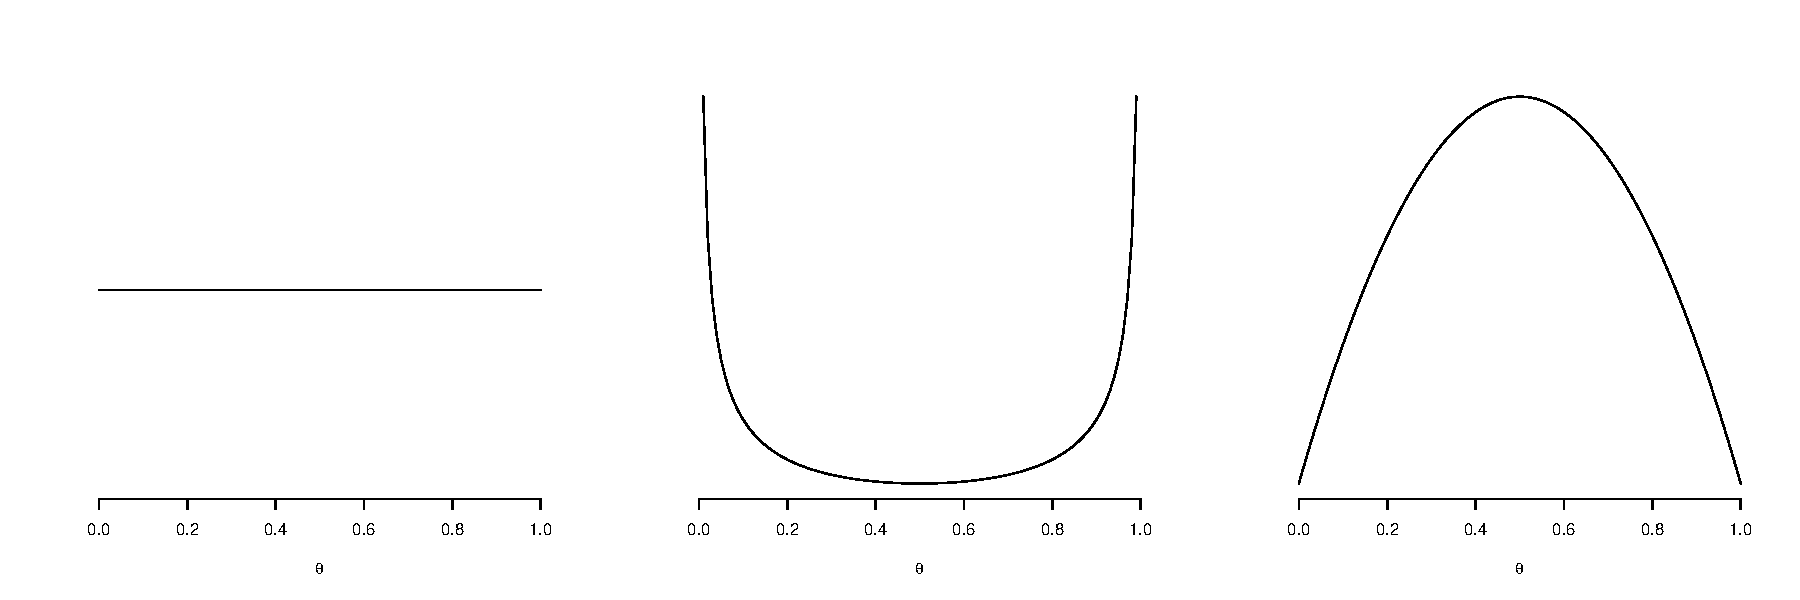
\includegraphics[width=\textwidth]{Files/Images/priorDistributions.pdf}
\end{center}

\question{
    Interpret the three \concept{prior distributions} above and discuss what information about the probability $\theta$ of the coin occurring on heads they incorporate.
}

\twolineanswerbox

\clearpage % Page break

When estimating a proportion (like the probability of heads in a coin toss) you can use the common $Beta(\alpha,\, \beta)$ distribution as a prior distribution on $\theta$ since it is restricted to the range [0, 1]. The $Beta(\alpha,\, \beta)$ distribution has two parameters, $\alpha$ and $\beta$, that have an effect on its shape. By playing around with these parameters, you can create the \concept{prior distribution} that reflects your particular beliefs as accurately as possible. \\

Run the following code in \texttt{R} to create the \concept{prior distribution} shown on the left of the figure above: \\

\codeblock{alpha <- 1 \\
beta <- 1 \\
curve(dbeta(x, alpha, beta), xlab = expression(theta), ylab = \textquotesingle\textquotesingle, yaxt = \textquotesingle n\textquotesingle)}

\question{Recreate the middle and right \concept{prior distributions} from the figure by changing the values for \rcode{alpha} and \rcode{beta} and running the code again. What are the values of $\alpha$ and $\beta$ for these distributions?}

\rcodeanswersmall

\emptyanswerbox{
    Middle: \hspace*{5cm} Right \\
    \\
    $\alpha$: \shortanswerline  \hspace*{2.5cm} $\alpha$: \shortanswerline
    \answerbreak
    $\beta$: \shortanswerline \hspace*{2.5cm} $\beta$: \shortanswerline
}

\question{How would you define a \concept{prior distribution} for $\theta$ if you believed the coin was definitely biased towards heads? And for one that is biased towards tails? Draw these \concept{prior distributions} below.}

\emptyanswerbox{
    \vspace*{-.5cm}
    \hspace*{2.1cm} Biased towards heads: \hspace*{0.65cm} Biased towards tails:
    \vspace*{-7.5pt}
    \begin{center}
        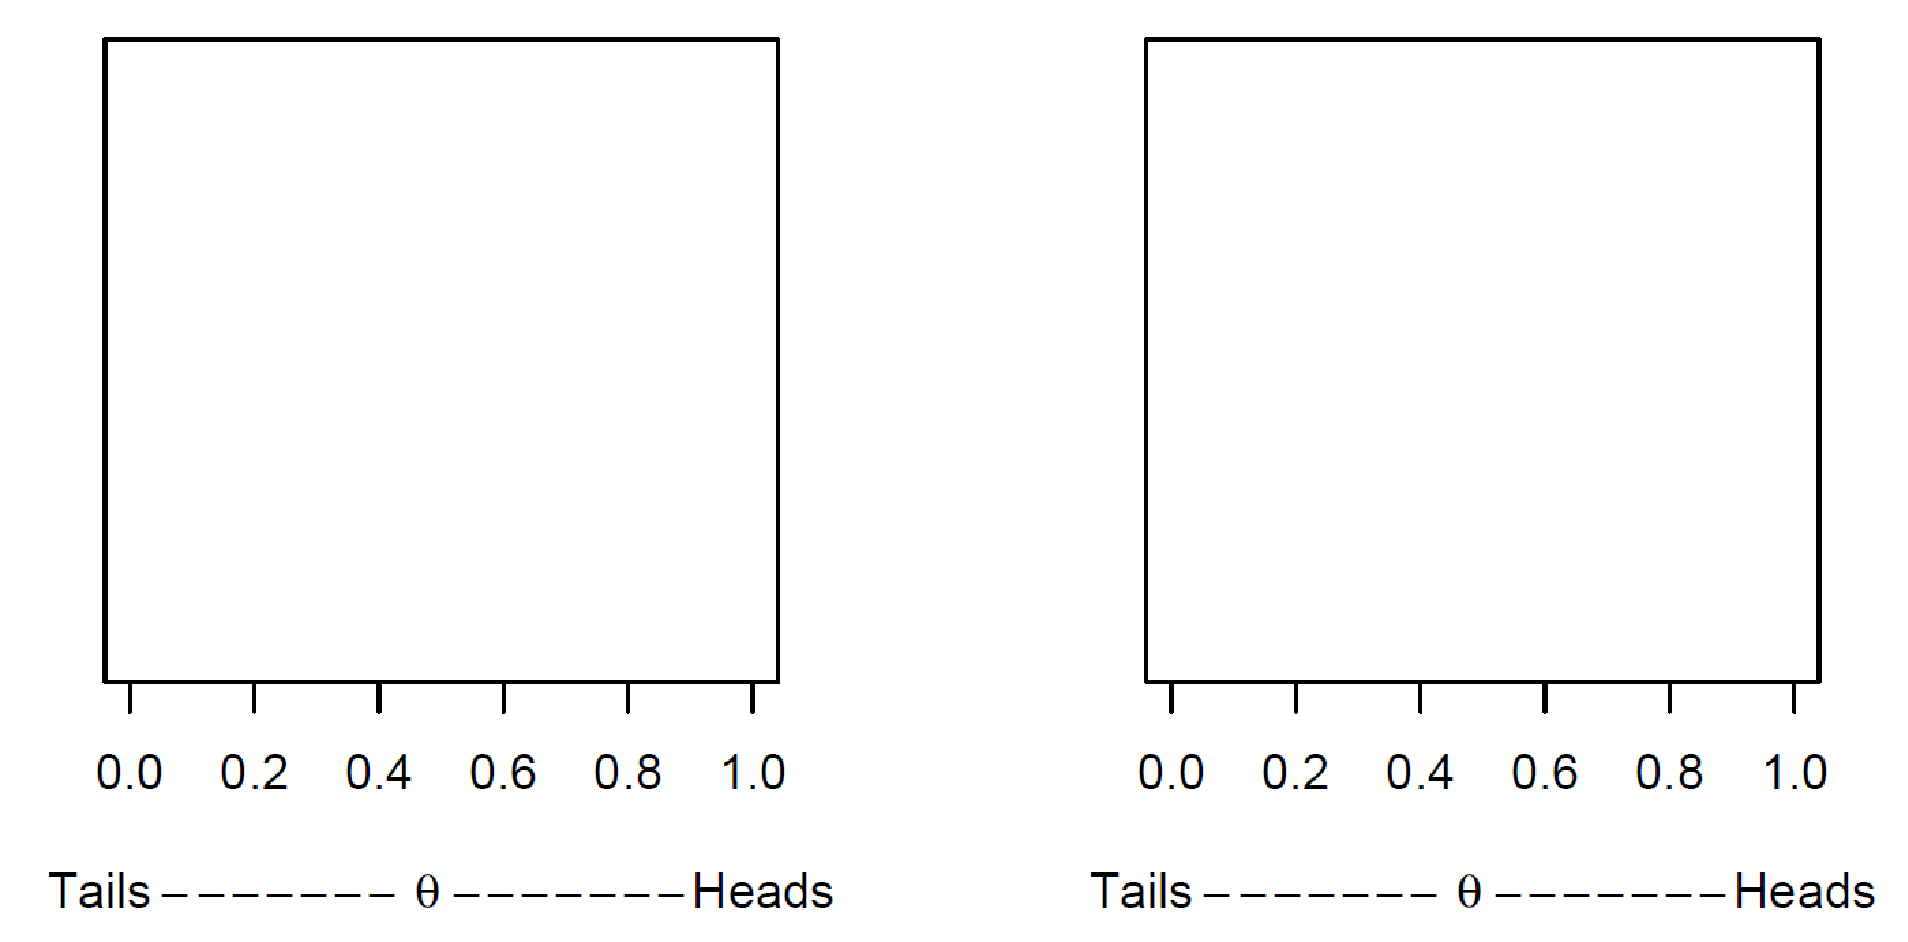
\includegraphics[height=5.3cm]{Files/Images/priorDistributionsAnswerField.pdf}
    \end{center}
}

\clearpage % Page break
\setcounter{section}{8}
\setcounter{subsection}{2}
\setcounter{question}{0}

%%%%%%%%%%%%%%%%%%%%%%%%%%%%%%%%%%%%%%%%%%%%%%%%%%%%%%%%%%%%%%%%%%%%%%%%%%%
% Assignment 8.2: Updating a prior distribution to a posterior distribution
%%%%%%%%%%%%%%%%%%%%%%%%%%%%%%%%%%%%%%%%%%%%%%%%%%%%%%%%%%%%%%%%%%%%%%%%%%%

\rassignment{Updating a prior distribution to a posterior distribution}

Suppose you are the manager of a small store and want to estimate what proportion of your customers leaves the store with a feeling of satisfaction. You give out a questionnaire to 40 people in the store and ask them whether they felt satisfied or not. In a previous enquiry done by you, it was already shown that, on average, 60\% of your customers feels good about the store, with a \concept{standard deviation} of ten percent. Using Bayesian statistics, you are now going to update the information from your previous enquiry with the information from the new questionnaire. \\

\question{What \concept{parameter} does $\theta$ represent in this scenario?}

\hint{Think about what question you are interested in answering.}

\onelineanswerbox

\question{Think of your own $\alpha$ and $\beta$ parameters for the $Beta(\alpha, \,\beta)$ \concept{prior distribution} on $\theta$. Take into account the average percentage from your previous enquiry and incorporate this into your \concept{prior distribution.}}

\emptyanswerbox{
    $\alpha$: \shortanswerline \hspace*{3cm} $\beta$: \shortanswerline
}

\question{Use the \rcode{curve()} function to create a figure of your \concept{prior distribution} in \texttt{R}.}

\rcodeanswertiny

By updating the $Beta(\alpha,\, \beta)$ prior distribution with information that you have collected, you create a \concept{posterior distribution}, which contains both the prior information and the information from the sample. Having observed $k$ successes in a sample of $n$ observations, the \concept{prior parameters} $\alpha$ and $\beta$ are updated to the \concept{posterior parameters} $\alpha + k$ and $\beta + n - k$. \\

In your sample of $n = 40$ questioned customers, $k = 33$ said they felt satisfied when leaving the store. \\

\clearpage % Page break

\question{Write down the \concept{parameters} of the \concept{posterior distribution}.}

\emptyanswerbox{
    $\alpha$: \shortanswerline \hspace*{3cm} $\beta$: \shortanswerline
}

Run the following code in \texttt{R} to create a figure of the \concept{posterior distribution}. Fill in your own values of \rcode{alpha} and \rcode{beta} from assignment 8.2b. \\

\codeblock{alpha <- 7\\
beta <- 5\\
n <- 40\\
k <- 33\\
\\
curve(dbeta(x, alpha + k, beta + n - k), \\
\hspace*{35pt}xlab = expression(theta), ylab = \textquotesingle\textquotesingle, yaxt = \textquotesingle n\textquotesingle)}

\question{
    Find out the \concept{posterior probability} that more than 60 percent of your customers left the store feeling satisfied, given the prior information and the information from the sample.
}

\hint{Use the \rcode{qbeta()} function to find the cumulative probability under a beta distribution.}

\rcodeanswertiny

\emptyanswerbox{
    \vspace*{-5pt}
    Probability: \shortanswerline
}

\question{
    Find out the \concept{posterior probability} that the percentage of customers that left the store feeling satisfied, given the prior information and the information from the sample, lies between 70 and 90 percent.
}

\rcodeanswertiny

\emptyanswerbox{
    \vspace*{-5pt}
    Probability: \shortanswerline
}

\clearpage % Page break

\question{Change the values of \rcode{alpha} and \rcode{beta} in the code above so that you have a different \concept{prior distribution} and run the code again. Describe how robust the \concept{posterior distribution} is to changes in the prior distribution.}

\rcodeanswersmall

\threelineanswerbox

\clearpage % Page break
\setcounter{chapter}{8}
\setcounter{section}{3}
\setcounter{question}{0}

%%%%%%%%%%%%%%%%%%%%%%%%%%%%%%%%%%%%%%%%%%%%%%%%%%%%%%%%%%%%%%%%%%%%%%%%%%%
% Assignment 8.3: Finding the posterior distribution using MCMC sampling
%%%%%%%%%%%%%%%%%%%%%%%%%%%%%%%%%%%%%%%%%%%%%%%%%%%%%%%%%%%%%%%%%%%%%%%%%%%

\rassignment{Finding the posterior distribution using MCMC sampling}

In assignment 8.2 you have seen that updating a \concept{prior distribution} to a \concept{posterior distribution} is easy when you are counting successes and failures. In this scenario the \concept{prior distribution} and \concept{posterior distribution} are in the same family, they are both $Beta$ distributions. However, many posterior distributions are not so easy to find. In this assignment, you are going to learn how to use a Markov chain Monte Carlo sampling method to approximate the posterior distribution for any combination of \concept{prior distributions} and \concept{likelihoods}. \\

For this exercise you will be using the \texttt{Stan} coding language with the \rcode{rstan} \texttt{R} package. \rcode{rstan} performs MCMC sampling using an Hamiltonian Monte Carlo (HMC) algorithm, which is known to have a very high quality in finding the \concept{posterior distribution}. Install and load the package using: \\
\\
\codeblock{install.packages(rstan) \\
library(rstan)}

\texttt{Stan} requires very specific commands. It requires that you specify all \rcode{data}, all \rcode{parameters}, and the complete statistical \rcode{model}\footnote{For a complete introduction to \texttt{Stan}, you can visit \url{https://github.com/stan-dev/rstan/wiki/RStan-Getting-Started}}. \\

Copy and run the following code in \texttt{R} to set up the \texttt{Stan} model for the scenario in exercise 8.2b and store it in an object called \rcode{modelCode}. The code then compiles the model using the \rcode{stan\_model()} function and starts sampling using the \rcode{sampling()} function. The result of the sampling is stored in the \rcode{stanFit} object. \\

\hint{You can change the \rcode{theta {\raise.17ex\hbox{$\scriptstyle\sim$}} beta(7, 5)} part of the code to specify your own prior distribution from assignment 8.2b.}

\codeblock{modelCode <- {\color{dataset}\textquotesingle} \\
{\color{dataset}data \{} \\
    \hspace*{20pt} {\color{dataset}int n;} \\
    \hspace*{20pt} {\color{dataset}int k;} \\
{\color{dataset}\}} \\
{\color{dataset}parameters \{ }\\
    \hspace*{20pt} {\color{dataset}real<lower=0,upper=1> theta; }\\
{\color{dataset}\}} \\
{\color{dataset}model \{ }\\
    \hspace*{20pt} {\color{dataset}theta {\raise.17ex\hbox{$\scriptstyle\sim$}} beta(7, 5); }\\
    \hspace*{20pt} {\color{dataset}k {\raise.17ex\hbox{$\scriptstyle\sim$}} binomial(n, theta); }\\
{\color{dataset} \} } \\
{\color{dataset}\textquotesingle} \\
\\
{\color{dataset}\# Note: The following line can take a while to execute}\\
compiledModel <- stan\_model(model\_code = modelCode, model\_name = \textquotesingle model\textquotesingle) \\
\\
stanFit <- sampling(compiledModel, data = list(n = 40, k = 33), \\ 
                    \hspace*{110pt}iter = 5000, warmup = 500, chains = 4)}

\clearpage % Page break

\question{Extract the samples of the \concept{posterior distribution} on $\theta$ from the \rcode{stanFit} object using the \rcode{extract()} function and store them in an object called \rcode{samples}.}

\rcodeanswertiny

\question{Create a histogram of the \rcode{samples}. Next, run the following code in \texttt{R} to plot the analytical \concept{posterior distribution} over the histogram. Do the samples of the \concept{posterior distribution} resemble the actual \concept{posterior distribution} in any way?}

\codeblock{curve(dbeta(x, shape1 = 40, shape2 = 12), add = TRUE)}

\hint{Be sure to specify a larger value for the \rcode{breaks} argument since you have many samples. Also set \rcode{probability = TRUE} in the \rcode{hist()} function.}

\rcodeanswersmall

\twolineanswerbox

As you have seen in assignment 8.2, the \concept{posterior distribution} you just estimated can be calculated by hand, since it is a $Beta$ distribution. However, to represent your prior information (remember: you have conducted a questionnaire that showed you 60 percent of customers left your store satisfied with a \concept{standard deviation} of 10 percent), let's give $\theta$ a $Normal(\mu,\, \sigma)$ distribution as a prior distribution. You use your prior estimate of $\theta$ as the \concept{mean} of the prior distribution, and the \concept{standard deviation} of the sample ($s = 0.10$) as the \concept{standard deviation} of the \concept{prior distribution}. \\

\question{Change the prior distribution in the \rcode{modelCode} to the $Normal$ distribution described in the text above. Run all appropriate code again.}

\hint{The line \rcode{theta {\raise.17ex\hbox{$\scriptstyle\sim$}} beta(7, 5)} specifies the prior distribution.}

\clearpage % Page break

\rcodeanswermedium

\question{Again, find out the \concept{posterior probability} that more than 60 percent of your customers left the store feeling satisfied, given the prior information and the information from the sample.}

\hint{Do \underline{not} use the \rcode{quantile()} function or the \rcode{pbeta()} function.}

\rcodeanswertiny

\emptyanswerbox{
    \vspace*{-5pt}
    Probability: \shortanswerline
}

\question{
    Find out the \concept{posterior probability} that the percentage of customers that left the store feeling satisfied, given the prior information and the information from the sample, lies between 70 and 90 percent.
}

\rcodeanswertiny

\emptyanswerbox{
    \vspace*{-5pt}
    Probability: \shortanswerline
}

\question{Do your answers for assignment 8.3d and assignment 8.3e differ substantially from your answers at assignment 8.2e and assignment 8.2f. What does this tell you about the robustness of your outcomes to the choice of \concept{prior distribution}?}

\twolineanswerbox

\clearpage % Page break
\setcounter{section}{8}
\setcounter{subsection}{4}
\setcounter{question}{0}

%%%%%%%%%%%%%%%%%%%%%%%%%%%%%%%%%%%%%%%%%%%%%%%%%%%%%%%%%%%%%%%%%%%%%%%%%%%
% Assignment 8.4: Comparing simple models using the Bayes factor
%%%%%%%%%%%%%%%%%%%%%%%%%%%%%%%%%%%%%%%%%%%%%%%%%%%%%%%%%%%%%%%%%%%%%%%%%%%

\rassignment{Comparing simple models using the Bayes factor}

Bayesian statistics does not use the \concept{p-value} to test hypotheses and yield conclusions in an all-or-none fashion. Instead it uses a continuous measure of evidence, the \concept{Bayes factor}. The \concept{Bayes factor} quantifies the relative predictive performance of two competing hypotheses; the \concept{null hypothesis} $H_0$ and the \concept{alternative hypothesis} $H_1$. The subscript in the \concept{Bayes factor} indicates for which hypothesis supported is quantified. $BF_{10}$ indicates the Bayes factor in favor of $H_1$ over $H_0$, whereas $BF_{01}$ indicates the \concept{Bayes factor} in favor of $H_0$ over $H_1$. Larger values of $BF_{10}$ indicate more support for $H_1$. A \concept{Bayes factor} can range from 0 to $\infty$, and a Bayes factor of 1 indicates that both hypotheses are supported equally well by the data. A $BF_{10} = 10$ indicates that the data is 10 times more likely to occur under $H_1$ than under $H_0$. This way, the Bayes factor is a continuous measure for the strength of evidence. \\

Suppose you are a data scientist at a stock trading company. You have written an algorithm that trades stocks automatically. Your algorithm either makes a profitable trade, or a losing trade. You want to make sure that your algorithm actually does something intellectual, and want to disprove the hypothesis that your algorithm makes a profitable trade with a probability other than if it were to trade stocks randomly. \\

\question{Specify the \concept{null hypothesis} $H_0$ and the \concept{alternative hypothesis} $H_1$ for the test of a proportion against a chance value.}

\hypothesesbox

\question{Specify a $Beta$ prior distribution for the \concept{parameter} $\theta$. Let your prior distribution depend on how much confidence you have in your programming skills.}

\hint{Think about what the $\theta$ represents in this case.}

\emptyanswerbox{
\begin{center}
    $\theta \sim Beta($\tinyanswerline, \tinyanswerline)
\end{center}
}

You monitor the algorithm for 30 trades, and each time mark a trade as a success (profit) or a failure (loss). After data collection you see that, of the 30 trades, your algorithm made 22 profitable trades. \\

\question{
    What are the $\alpha$ and $\beta$ parameters of your \concept{posterior distribution}?
}

\emptyanswerbox{
    $\alpha$: \shortanswerline \hspace*{3cm} $\beta$: \shortanswerline
}

\clearpage % Page break

\question{Use the \rcode{curve()} function to create a figure that has both the prior and the posterior distribution in it.}

\hint{The \rcode{curve()} function has an argument \rcode{add} that controls whether to add a line to an already existing plot.}

In this scenario, the \concept{Bayes factor} is intuitively to calculate by only looking at the posterior distribution for $H_1$. The \concept{Bayes factor} $BF_{10}$ tells you how much more likely the \concept{alternative hypothesis} $H_1$ is in comparison with to the point \concept{null hypothesis} $H_0$. The \concept{Bayes factor} $BF_{10}$ in favor of the unrestricted \concept{alternative hypothesis} $H_1: \theta \neq 0.5$ is simply the height of the \concept{posterior distribution} at the point $\theta = 0.5$ divided by the height of the \concept{prior distribution} at the point $\theta = 0.5$. \\

Please note that this is a trick that only works for \concept{nested} hypotheses and models, in which only one of the \concept{parameters} is fixed to a specific value. \\

\begin{center}
    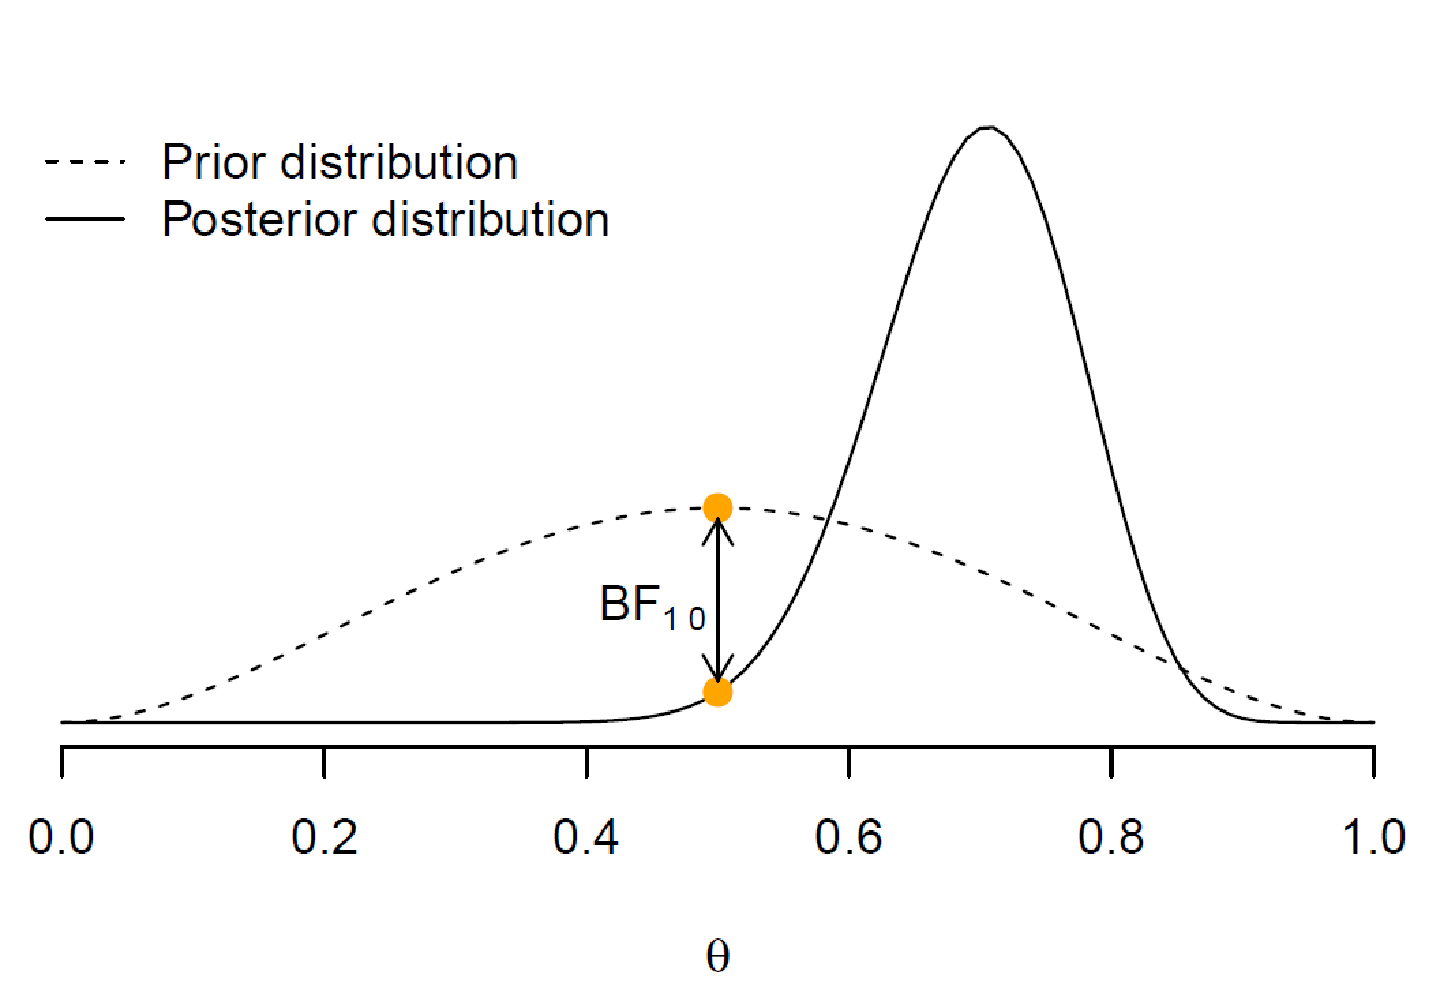
\includegraphics[width=0.8\textwidth]{Files/Images/priorAndPosterior.pdf}
\end{center}

\question{Use the \rcode{dbeta()} function to find out the height of your \concept{prior distribution} at the point $\theta = 0.5$ and store it in an object called \rcode{heightPrior}.}

\rcodeanswertiny

\question{Use the \rcode{dbeta()} function to find out the height of your \concept{posterior distribution} at the point $\theta = 0.5$ and store it in an object called \rcode{heightPosterior}.}

\rcodeanswertiny

\clearpage % Page break

Run the following code in \texttt{R} to compute the \concept{Bayes factor} in favor of the \concept{alternative hypothesis} $H_1$. \\
\\
\codeblock{BF10 <- heightPrior / heightPosterior}

\question{What is the value of the \concept{Bayes factor} \rcode{BF10}? Interpret this \concept{Bayes factor} with respect to the alternative hypothesis $H_1$.}

\twolineanswerbox

To make interpretation of the \concept{Bayes factor} more simple, the labels in the table below have been proposed. Please note that you shout not get too hung up on the specific labels and breakpoints in this table, since convincing evidence is different for every situation. \\

\begin{table}[h]
    \centering
    \begin{tabular}{r|l}
         Bayes factor & Evidence \\
         \hline
         1 - 3 & Anecdotal \\
         3 - 10 & Moderate \\
         10 - 30 & Strong \\ 
         30 - 100 & Very strong \\
         $>$ 100 & Extreme
    \end{tabular}
\end{table}

\question{Considering the labels from the table above, can you convincingly disprove the hypothesis that your algorithm makes a profitable trade with a probability other than if it were to trade stocks randomly?}

\twolineanswerbox

\question{Re-specify the $\alpha$ and $\beta$ parameters of the \concept{prior distribution} so that you express a different prior belief. Recalculate the \concept{Bayes factor} by running your code again. What is the new value of \rcode{BF10}. How robust in your \concept{Bayes factor} to changes in the prior distribution?}

\onelineanswerbox

\clearpage % Page break
\setcounter{chapter}{8}
\setcounter{section}{5}
\setcounter{question}{0}

%%%%%%%%%%%%%%%%%%%%%%%%%%%%%%%%%%%%%%%%%%%%%%%%%%%%%%%%%%%%%%%%%%%%%%%%%%%
% Assignment 8.5: Using bridge sampling to calculate the Bayes factor
%%%%%%%%%%%%%%%%%%%%%%%%%%%%%%%%%%%%%%%%%%%%%%%%%%%%%%%%%%%%%%%%%%%%%%%%%%%

\rassignment{Using bridge sampling to calculate the Bayes factor}

You are not convinced by the evidence from assignment 8.4 and want to perform additional testing. This time, however, you want to find out whether your algorithm makes more than 75 percent of the trades with profit. That is, you want to test whether $\theta$ is higher or lower than 0.75.\\

\question{Formulate the \concept{models} $M_1$ (restricts $\theta$ to be below 0.75) and $M_2$ (restricts $\theta$ to be higher than 0.75). Choose the restriction ($\leq$, $=$, or $\geq$) that applies to each model.}

\emptyanswerbox{
    $M_1$: $\theta \leq / = / \geq$ \tinyanswerline \hspace{3cm} $M_2$: $\theta \leq / = / \geq$ \tinyanswerline
}

For these more complicated (e.g., non-nested) models, the computation of the \concept{Bayes factor} becomes more difficult since it involves computing the \concept{marginal likelihoods} of the \concept{models}. To make your life simple, you can use the \rcode{bridgesampling} package together with the \rcode{rstan} package to let \texttt{R} calculate these values for you. \\

Run the following code in \texttt{R} to install the \rcode{bridgesampling} package. Then load the \rcode{bridgesampling} and the \rcode{rstan} package. \\
\\
\codeblock{install.packages(\textquotesingle bridgesampling\textquotesingle) \\
            \\
            library(bridgesampling) \\
            library(rstan)}

Copy and run the following code in \texttt{R} to set up the \texttt{Stan} model for $M_1$, the model that restricts $\theta$ to be lower than 0.75 and store it in an object called \rcode{model1}. The code then compiles the model using the \rcode{stan\_model()} function. \\
\\
\codeblock{model1code <- {\color{dataset}\textquotesingle} \\
{\color{dataset}data \{} \\
    \hspace*{20pt} {\color{dataset}int n;} \\
    \hspace*{20pt} {\color{dataset}int k;} \\
{\color{dataset}\}} \\
{\color{dataset}parameters \{ }\\
    \hspace*{20pt} {\color{dataset}real<lower=0,upper=0.75> theta; }\\
{\color{dataset}\}} \\
{\color{dataset}model \{ }\\
    \hspace*{20pt} {\color{dataset}theta {\raise.17ex\hbox{$\scriptstyle\sim$}} beta(1, 1)T[0, 0.75]; }\\
    \hspace*{20pt} {\color{dataset}k {\raise.17ex\hbox{$\scriptstyle\sim$}} binomial(n, theta); }\\
{\color{dataset} \} } \\
{\color{dataset}\textquotesingle} \\
\\
{\color{dataset}\# Note: The following line can take a while to execute}\\
model1 <- stan\_model(model\_code = model1code, model\_name = \textquotesingle model1\textquotesingle) }

\clearpage % Page break

\question{Create the \texttt{Stan} model for $M_2$, the model that restricts $\theta$ to be higher than 0.75, on the basis of the lines in \rcode{model1code}. Name the compiled model \rcode{model2}.}

\hint{First find out what elements were added to the code since assignment 8.3.}

\rcodeanswerlarge

\question{Locate and describe the \concept{prior distributions} for $\theta$ in $M_1$ and $M_2$.}

\twolineanswerbox

Now you start collecting data again. Suppose that you monitor your algorithm for $n = 156$ more trades, and find that $k = 123$ trades resulted in a profit. \\

\question{Use the \rcode{sampling()} function to sample for the \concept{models} $M_1$ and $M_2$ using these data. Store the fitted \texttt{Stan} models in objects named \rcode{stanFitM1} and \rcode{stanFitM2}.}

\rcodeanswersmall

\question{Use the \rcode{bridge\_sampler()} function to calculate the \concept{marginal likelihoods} of the models $M_1$ and $M_2$ and store them in \rcode{mLike1} and \rcode{mLike2}.}

\rcodeanswersmall

\clearpage % Page break

\question{Use the \rcode{bf()} function to calculate the \concept{Bayes factor} $BF_{21}$ in favor of model $M_2$ over model $M_1$ and store it in an object called \rcode{BF21}.}

\hint{Be sure to insert the two marginal likelihoods into the \rcode{bf()} function in the correct order so that the result is $BF_{21}$.}

\question{What is the value of \rcode{BF21}? Interpret this \concept{Bayes factor} with respect to the model that restricts $\theta$ to be higher than 0.75.}

\threelineanswerbox

\question{What is the strength of evidence associated with this \concept{Bayes factor}? Are you convinced by this evidence?}

\threelineanswerbox

\clearpage % Page break
\setcounter{chapter}{8}
\setcounter{section}{6}
\setcounter{question}{0}

%%%%%%%%%%%%%%%%%%%%%%%%%%%%%%%%%%%%%%%%%%%%%%%%%%%%%%%%%%%%%%%%%%%%%%%%%%%
% Assignment 8.6: Performing a Bayesian linear regression
%%%%%%%%%%%%%%%%%%%%%%%%%%%%%%%%%%%%%%%%%%%%%%%%%%%%%%%%%%%%%%%%%%%%%%%%%%%

\rassignment{Performing a Bayesian linear regression}

Suppose you work as an analyst for an insurance firm. Your firm wants to assess which variables can predict the height of of a customer insurance charges. For this assignment you will need the \dataset{insurance.csv}\footnote{These data are adapted from the original open-source data set which can be found at: \url{https://www.kaggle.com/mirichoi0218/insurance/data}.} from the online resources. The data set contains a sample of 1338 health insurance customer and their recorded variables. For the current assignment, you can focus on the columns \rcode{charges} (the total charges of the customer), \rcode{age} (the customer age), \rcode{bmi} (the customer BMI score), and \rcode{neighbors} (the number of neighbors of the customer) columns. \\

\question{
    Use the \rcode{read.csv()} function (and \rcode{setwd()} function if you prefer) to import the data set into an object named \rcode{insurance}.
}

\rcodeanswertiny

\question{
    Write down the regression equation for a \concept{linear model} where you predict the variable \rcode{charges} on the basis of the predictor variables \rcode{age}, \rcode{bmi}, and \rcode{neighbors}.
}

\emptyanswerbox{
    charges = \longanswerline
}

Run the following code in \texttt{R} to create a \texttt{Stan} model $M_1$ that corresponds to this linear model with all \concept{coefficients}. Note that you do not specify \concept{prior distributions} (under the \rcode{model} section) for the $\beta_0$, $\beta_1$, and $\beta_2$ parameters. That is because, when you do not specify the prior distributions in \rcode{Stan}, the posterior distributions will be estimated solely from the data. \\

\clearpage % Page break

\codeblock{regmodelcode <- {\color{dataset}\textquotesingle} \\
{\color{dataset}data \{} \\
    \hspace*{20pt} {\color{dataset}int<lower=0> N;} \\
    \hspace*{20pt} {\color{dataset}vector[N] x1;} \\
    \hspace*{20pt} {\color{dataset}vector[N] x2;} \\
    \hspace*{20pt} {\color{dataset}vector[N] x3;} \\
    \hspace*{20pt} {\color{dataset}vector[N] y;} \\
{\color{dataset}\}} \\
{\color{dataset}parameters \{ }\\
    \hspace*{20pt} {\color{dataset}real beta0; }\\
    \hspace*{20pt} {\color{dataset}real beta1; }\\
    \hspace*{20pt} {\color{dataset}real beta2; }\\
    \hspace*{20pt} {\color{dataset}real beta3; }\\
    \hspace*{20pt} {\color{dataset}real<lower=0> sigma; }\\
{\color{dataset}\}} \\
{\color{dataset}model \{ }\\
    \hspace*{20pt} {\color{dataset}y {\raise.17ex\hbox{$\scriptstyle\sim$}} normal(beta0 + beta1 * x1 + beta2 * x2 + beta3 * x3, sigma);}\\
{\color{dataset} \} } \\
{\color{dataset}\textquotesingle} \\
\\
{\color{dataset}\# Note: The following line can take a while to execute}\\
regressionModel <- stan\_model(model\_code = regmodelcode, model\_name = \textquotesingle Regression\textquotesingle) }

\question{
    Use the \rcode{sampling()} function to sample from the \rcode{regressionModel} model and store the samples in an object named \rcode{regressionSamples}. Next, use the \rcode{summary()} function to find out the \concept{posterior means} of the $\beta_0$, $\beta_1$, $\beta_2$, and $\beta_3$ coefficients. 
}

\emptyanswerbox{
    \vspace*{-7.5pt}
    $\beta_0$: \tinyanswerline \hspace*{1cm} $\beta_1$: \tinyanswerline \hspace*{1cm} $\beta_2$: \tinyanswerline \hspace*{1cm} $\beta_3$: \tinyanswerline
}

\rcodeanswersmall

\question{Use the \rcode{lm()} function to fit a regular \concept{linear model} to the data. Use the \rcode{summary()} function to find out the estimates of the coefficients when done this way. Do they match the \concept{posterior means} from assignment 8.6b?}

\rcodeanswertiny

\clearpage % Page break

\emptyanswerbox{
    \vspace*{-15pt}
    \begin{center}
        YES / NO
    \end{center}
}

Run the following code in \texttt{R} to create a figure of the posterior distribution of $\beta_1$, the regression coefficient for the variable \rcode{age}: \\
\\
\codeblock{plot(density(regressionSamples\$beta1), xlab = \textquotesingle \textquotesingle, ylab = \textquotesingle \textquotesingle, \\
\hspace*{30pt}yaxt = \textquotesingle n\textquotesingle, bty = \textquotesingle n\textquotesingle, main = expression(beta[1]))}

\question{
    Also create figures of the posterior distributions for $\beta_0$, $\beta_2$, and $\beta_3$.
}

\rcodeanswersmall

\question{Find out the probability that the average increase in \rcode{charges} as a function of 1 point on the \rcode{bmi} scale is higher than 200 dollars.}

\hint{Use the approach that you applied in assignment 8.3d and assignment 8.3e.}

\rcodeanswertiny

\emptyanswerbox{
    Probability: \shortanswerline
}

\question{
    Find out the probability that the value of $\beta_1$ is lower than 250.
}

\rcodeanswertiny

\emptyanswerbox{
    Probability: \shortanswerline
}

\clearpage % Page break

\question{
    Find out between which values of $\beta_3$ 90 percent of the \concept{posterior samples} lie. 
}

\rcodeanswertiny

\emptyanswerbox{
    Lower bound: \shortanswerline \hspace*{1cm} Upper bound: \shortanswerline
}

As you can see, the posterior distribution for the $\beta_3$ coefficient centers around zero, and it's contribution to the accuracy of the prediction can be questioned. To test how much more likely a model is that includes the $\beta_3$ predicts the data compared to a model that excludes the coefficient, you can use the procedure that you have learned in assignment 8.5. \\

\question{
    Write code for a new \texttt{Stan} model $M_2$ where you remove the predictor variable \rcode{neighbors}.
}

\rcodeanswerlarge

\question{
    Using the procedure in assignment 8.5, calculate the \concept{Bayes factor} $BF_{12}$ in favor of $M_1$ (the model that includes $\beta_3$) over $M_2$ (the model that excludes $\beta_3$). 
}

\rcodeanswermedium

\clearpage % Page break

\question{What is the value of $BF_{12}$. Interpret this \concept{Bayes factor} with respect to the coefficient $\beta_0$. Incorporate the strength of the evidence in your answer.}

\fourlineanswerbox

Keep in mind that basically all statistical tests are a specific form of regression (like you have learned in chapter 6). This means that you can extend the \texttt{Stan} models that you have seen in this chapter to answer any question that you want to investigate.

\clearpage % Page break 
\clearpage

% Formula sheet and tables
\addtocontents{toc}{\newpage\protect\vspace{10pt}}
\section{Formula sheet and tables}
\label{formulasheet}

\begin{minipage}[t]{.45\textwidth}
\begin{center}
    \textbf{Central tendency}
\end{center}
\hline
\answerskip
Mean \hfill $\bar{x} = \frac{\sum^n_{i = 1} x_i}{n}$ \\
\\
Median ($Q_2$) \hfill $\frac{(n + 2)}{2}th number$ \\
\\
Lower quartile ($Q_1$) \hfill $\frac{(n + 2)}{4}th number$ \\
\\
Upper quartile ($Q_1$) \hfill $\frac{(n + 2)}{4} \times 3\, th number$ \\
\\
Range \hfill $max_x - min_x$ \\
\\
Interquartile range \hfill $Q_3 - Q_1$ \\
\\
\begin{center}
    \textbf{Dispersion}
\end{center}
\hline
\answerskip
Variance \hfill $s^2 = \frac{\sum^n_{i = 1} (x_i - \bar{x})^2}{n - 1}$ \\
\\
Standard deviation \hfill $s = \sqrt{s^2}$ \\
\\
Hartley's F \hfill $F = \frac{var_{max}}{var_{min}} = \frac{s^2_{max}}{s^2_{min}}$\\
\\
\begin{center}
    \textbf{Confidence intervals}
\end{center}
\hline
\answerskip
Standard error \hfill $SE_\mu = \frac{s}{\sqrt{n}}$ \\
{\scriptsize (of the sample mean)}\\
\\
Confidence interval \hfill $\bar{x} \pm z_\alpha \times SE_\mu$ \\
{\scriptsize (for the population mean with $n \geq 30$)}\\
\\
Confidence interval \hfill $\bar{x} \pm t_\alpha \times SE_\mu$ \\
{\scriptsize (for the population mean with $n < 30$)}\\
\\
Confidence interval \hfill $p \pm t_\alpha \times \sqrt{\frac{p(1 - p)}{n}}$ \\
{\scriptsize (for the population proportion)}\\
\end{minipage}
\hfill\vline\hfill
\begin{minipage}[t]{.45\textwidth}
\begin{center}
    \textbf{Tests based on the normal distribution}
\end{center}
\hline
\answerskip
z-score \hfill $z = \frac{x - \mu}{\sigma}$\\
{\scriptsize (for a value $x$ in a normal distribution)} \\
\\
z-score \hfill $z = \frac{\bar{x} - \mu}{\nicefrac{s}{\sqrt{n}}}$\\
{\scriptsize (for a test of a population mean based on a sample)} \\
\begin{center}
    \textbf{Tests based on the t-distribution}
\end{center}
\hline
\answerskip
t-score: \hfill $t = \frac{\bar{x} - \mu}{\nicefrac{s}{\sqrt{n}}}$\\
{\scriptsize (for a test of a population mean based on sample $n < 30$)} \\
\\
Degrees of freedom: \hfill $df = n - 1$\\
{\scriptsize (for the t-distribution in a one sample t-test)} \\
\\
t-score: \hfill $t = \frac{(\bar{x_1} - \bar{x_2}) - D_0}
{\sqrt{s^2_p (\frac{1}{n_1} + \frac{1}{n_2})}}$\\
{\scriptsize (for an independent samples t-test)} \\
\\
Standard error: \hfill $s^2_p = \frac{(n_1 - 1) s^2_1 + (n_2 - 1) s^2_2}{n_1 + n_2 - 2}$\\
{\scriptsize (for an independent samples t-test)} \\
\\
Degrees of freedom: \hfill $df = n_1 + n_2 - 2$\\
{\scriptsize (for an independent samples t-test)} \\
\\
t-score: \hfill $t = \frac{\bar{D} - \mu_0}
{\nicefrac{s_D}{\sqrt{n}}}$\\
{\scriptsize (for a dependent samples t-test)} \\
\\
Degrees of freedom: \hfill $df =n - 1$\\
{\scriptsize (for a dependent samples t-test)} \\
\\
\begin{center}
    \textbf{Correlation}
\end{center}
\hline
\answerskip
Covariance \hfill $s_{xy} = \frac{\sum^n_{i = 1} (x_i - \bar{x})(y_i - \bar{y})}{n - 1}$\\
\\
Correlation \hfill $r_{xy} = \frac{s_{xy}}{s_x \times s_y}$ \\
\\
Sampling distribution: \hfill $z_r = \frac{1}{2} \times log_e (\frac{1 + r}{1 - r})$\\
{\scriptsize (for the population correlation)} \\
\\
Standard error: \hfill $SE_r = \frac{1}{\sqrt{n - 3}}$\\
{\scriptsize (of the population correlation)} \\
\\
\end{minipage}

\clearpage % Page break

\begin{minipage}[t]{.45\textwidth}
z-score: \hfill $z_{xy} = \frac{z_r}{SE_r}$\\
{\scriptsize (for the test of a correlation against any value)} \\
\\
Degrees of freedom: \hfill $df = n - 2$\\
{\scriptsize (for the t-distribution in correlation test against zero)} \\
\\
t-score: \hfill $t_{xy} = \frac{r \sqrt{n - 2}}{\sqrt{1 - r^2}}$\\
{\scriptsize (for the test of a correlation against zero)} \\
\\
\begin{center}
    \textbf{Regression and AN(C)OVA}
\end{center}
\hline
\answerskip
R-squared \hfill $R^2 = \frac{SS_M}{SS_R}$ \\
{\scriptsize (of a regression or AN(C)OVA)} \\
\\
F-score \hfill $F = \frac{MS_M}{MS_R}$ \\
{\scriptsize (of a regression or AN(C)OVA)} \\
\\
Degrees of freedom \hfill $df_M = k - 1$ \\
{\scriptsize (for the AN(C)OVA model)} \\
\\
Degrees of freedom \hfill $df_R = n - k$ \\
{\scriptsize (for the AN(C)OVA residuals)} \\
\\
Mean squared error \hfill $MS_M = \frac{SS_M}{df_M}$ \\
{\scriptsize (for the AN(C)OVA model)} \\
\\
Mean squared error \hfill $MS_R = \frac{SS_R}{df_R}$ \\
{\scriptsize (for the AN(C)OVA residuals)} \\
\\
\end{minipage}
\hfill\vline\hfill
\begin{minipage}[t]{.45\textwidth}
\begin{center}
    \textbf{Proportions}
\end{center}
\hline
\answerskip
Combined success probability \hfill $p^* = \frac{k_1 + k_2}{n_1 + n_}$ \\
{\scriptsize (for the outcomes of two samples)} \\
\\
Standard error \hfill $s_p = \sqrt{p^*(1 - p^*) (\frac{1}{n_1} + \frac{1}{n_2})}$ \\
{\scriptsize (for the proportion of two samples)} \\
\\
z-score \hfill $z = \frac{p_1 - p_2}{s_p}$ \\
{\scriptsize (for a test comparing two proportions)} \\
\\
Expected value \hfill $E = p \times n$ \\
{\scriptsize (for a proportion)} \\
\\
Chi-square score \hfill $X^2 = \sum_{i=1}^k \frac{(O - E)^2}{E}$ \\
{\scriptsize (for a test comparing $k$ proportions)} \\
\\
\end{minipage}                \clearpage
\subsection{Table 1: Critical values for Hartley’s F ($F_{max}$)}
\label{table1}

Level of significance $\alpha = 0.05$ \\
\begin{center}
\small
\begin{tabular}{c|c|c|c|c|c|c|c|c|c|c|c}
\hline
\multicolumn{12}{c}{\textbf{Number of variances to compare} ($k$)}                    \bstrut\tstrut\\
\hline
$n - 1$ & \multicolumn{1}{c}{\textbf{2}}    & \multicolumn{1}{c}{\textbf{3}}    & \multicolumn{1}{c}{\textbf{4}}    & \multicolumn{1}{c}{\textbf{5}}    & \multicolumn{1}{c}{\textbf{6}}    & \multicolumn{1}{c}{\textbf{7}}    & \multicolumn{1}{c}{\textbf{8}}    & \multicolumn{1}{c}{\textbf{9}}    & \multicolumn{1}{c}{\textbf{10}}   & \multicolumn{1}{c}{\textbf{11}}   & \multicolumn{1}{c}{\textbf{12}} \bstrut\tstrut\\
\hline
\textbf{2}     & 39.0 & 87.5 & 142  & 202  & 266  & 333  & 403  & 475  & 550  & 626  & 704  \bstrut\tstrut\\
\textbf{3}     & 15.4 & 27.8 & 39.2 & 50.7 & 62.0 & 72.9 & 83.5 & 93.9 & 104  & 114  & 124  \bstrut\tstrut\\
\textbf{4}     & 9.6  & 15.5 & 20.6 & 25.2 & 29.5 & 33.6 & 37.5 & 41.1 & 44.6 & 48.0 & 51.4 \bstrut\tstrut\\
\textbf{5}     & 7.15 & 10.8 & 13.7 & 16.3 & 18.7 & 20.8 & 22.9 & 24.7 & 26.5 & 28.2 & 29.9 \bstrut\tstrut\\
\textbf{6}     & 5.82 & 8.38 & 10.4 & 12.1 & 13.7 & 15.0 & 16.3 & 17.5 & 18.6 & 19.7 & 20.7 \bstrut\tstrut\\
\textbf{7}     & 4.99 & 6.94 & 8.44 & 9.70 & 10.8 & 11.8 & 12.7 & 13.5 & 14.3 & 15.1 & 15.8 \bstrut\tstrut\\
\textbf{8}     & 4.43 & 6.00 & 7.18 & 8.12 & 9.03 & 9.78 & 10.5 & 11.1 & 11.7 & 12.2 & 12.7 \bstrut\tstrut\\
\textbf{9}     & 4.03 & 5.34 & 6.31 & 7.11 & 7.80 & 8.41 & 8.95 & 9.45 & 9.91 & 10.3 & 10.7 \bstrut\tstrut\\
\textbf{10}    & 3.72 & 4.85 & 5.67 & 6.34 & 6.92 & 7.42 & 7.87 & 8.28 & 8.66 & 9.01 & 9.34 \bstrut\tstrut\\
\textbf{12}    & 3.28 & 4.16 & 4.79 & 5.30 & 5.72 & 6.09 & 6.42 & 6.72 & 7.00 & 7.25 & 7.48 \bstrut\tstrut\\
\textbf{15}    & 2.86 & 3.54 & 4.01 & 4.37 & 4.68 & 4.95 & 5.19 & 5.40 & 5.59 & 5.77 & 5.93 \bstrut\tstrut\\
\textbf{20}    & 2.46 & 2.95 & 3.29 & 3.54 & 3.76 & 3.94 & 4.10 & 4.24 & 4.37 & 4.49 & 4.59 \bstrut\tstrut\\
\textbf{30}    & 2.07 & 2.40 & 2.61 & 2.78 & 2.91 & 3.02 & 3.12 & 3.21 & 3.29 & 3.36 & 3.39 \bstrut\tstrut\\
\textbf{60}    & 1.67 & 1.85 & 1.96 & 2.04 & 2.11 & 2.17 & 2.22 & 2.26 & 2.30 & 2.33 & 2.36 \bstrut\tstrut\\
$\infty$      & 1.00 & 1.00 & 1.00 & 1.00 & 1.00 & 1.00 & 1.00 & 1.00 & 1.00 & 1.00 & 1.00 \bstrut\tstrut\\
\hline
\end{tabular}
\end{center}                      \clearpage
\subsection{Table 2: z - values for significance level $\alpha$}
\label{table2}

\vspace*{-30pt}
\begin{minipage}{0.6\textwidth}
\hfill
\end{minipage}
\begin{minipage}{0.4\textwidth}
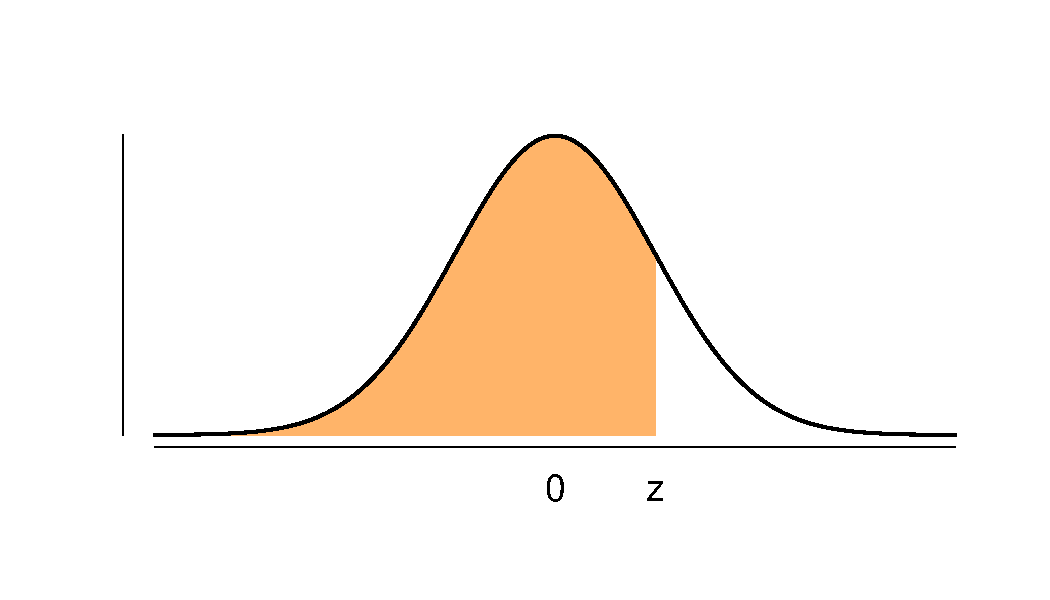
\includegraphics[width=\textwidth]{Files/Images/Normal.pdf}
\end{minipage}

\begin{center}
\small
\begin{tabular}{c|c|c|c|c|c|c|c|c|c|c}
\hline
\multicolumn{1}{c}{$z$}   & \multicolumn{1}{c}{\textbf{0.00}}    & \multicolumn{1}{c}{\textbf{0.01}}    & \multicolumn{1}{c}{\textbf{0.02}}    & \multicolumn{1}{c}{\textbf{0.03}}    & \multicolumn{1}{c}{\textbf{0.04}}    & \multicolumn{1}{c}{\textbf{0.05}}    & \multicolumn{1}{c}{\textbf{0.06}}    & \multicolumn{1}{c}{\textbf{0.07}}    & \multicolumn{1}{c}{\textbf{0.08}}    & \multicolumn{1}{c}{\textbf{0.09}}    \bstrut\tstrut\\
\hline
\textbf{0.0} & 0.5000  & 0.5040  & 0.5080  & 0.5120  & 0.5160  & 0.5199  & 0.5239  & 0.5279  & 0.5319  & 0.5359  \tstrut\\
\textbf{0.1} & 0.5398  & 0.5438  & 0.5478  & 0.5517  & 0.5557  & 0.5596  & 0.5636  & 0.5675  & 0.5714  & 0.5753  \\
\textbf{0.2} & 0.5793  & 0.5832  & 0.5871  & 0.5910  & 0.5948  & 0.5987  & 0.6026  & 0.6064  & 0.6103  & 0.6141  \\
\textbf{0.3} & 0.6179  & 0.6217  & 0.6255  & 0.6293  & 0.6331  & 0.6368  & 0.6406  & 0.6443  & 0.6480  & 0.6517  \\
\textbf{0.4} & 0.6554  & 0.6591  & 0.6628  & 0.6664  & 0.6700  & 0.6736  & 0.6772  & 0.6808  & 0.6844  & 0.6879  \\
\textbf{0.5} & 0.6915  & 0.6950  & 0.6985  & 0.7019  & 0.7054  & 0.7088  & 0.7123  & 0.7157  & 0.7190  & 0.7224  \\
\textbf{0.6} & 0.7257  & 0.7291  & 0.7324  & 0.7357  & 0.7389  & 0.7422  & 0.7454  & 0.7486  & 0.7518  & 0.7549  \\
\textbf{0.7} & 0.7580  & 0.7611  & 0.7642  & 0.7673  & 0.7704  & 0.7734  & 0.7764  & 0.7794  & 0.7823  & 0.7852  \\
\textbf{0.8} & 0.7881  & 0.7910  & 0.7939  & 0.7967  & 0.7995  & 0.8023  & 0.8051  & 0.8078  & 0.8106  & 0.8133  \\
\textbf{0.9} & 0.8159  & 0.8186  & 0.8212  & 0.8238  & 0.8264  & 0.8289  & 0.8315  & 0.8340  & 0.8365  & 0.8389  \\
\textbf{1.0} & 0.8413  & 0.8438  & 0.8461  & 0.8485  & 0.8508  & 0.8531  & 0.8554  & 0.8577  & 0.8599  & 0.8621  \\
\textbf{1.1} & 0.8643  & 0.8665  & 0.8686  & 0.8708  & 0.8729  & 0.8749  & 0.8770  & 0.8790  & 0.8810  & 0.8830  \\
\textbf{1.2} & 0.8849  & 0.8869  & 0.8888  & 0.8907  & 0.8925  & 0.8944  & 0.8962  & 0.8980  & 0.8997  & 0.9015  \\
\textbf{1.3} & 0.9032  & 0.9049  & 0.9066  & 0.9082  & 0.9099  & 0.9115  & 0.9131  & 0.9147  & 0.9162  & 0.9177  \\
\textbf{1.4 }& 0.9192  & 0.9207  & 0.9222  & 0.9236  & 0.9251  & 0.9265  & 0.9279  & 0.9292  & 0.9306  & 0.9319  \\
\textbf{1.5} & 0.9332  & 0.9345  & 0.9357  & 0.9370  & 0.9382  & 0.9394  & 0.9406  & 0.9418  & 0.9429  & 0.9441  \\
\textbf{1.6} & 0.9452  & 0.9463  & 0.9474  & 0.9484  & 0.9495  & 0.9505  & 0.9515  & 0.9525  & 0.9535  & 0.9545  \\
\textbf{1.7} & 0.9554  & 0.9564  & 0.9573  & 0.9582  & 0.9591  & 0.9599  & 0.9608  & 0.9616  & 0.9625  & 0.9633  \\
\textbf{1.8 }& 0.9641  & 0.9649  & 0.9656  & 0.9664  & 0.9671  & 0.9678  & 0.9686  & 0.9693  & 0.9699  & 0.9706  \\
\textbf{1.9} & 0.9713  & 0.9719  & 0.9726  & 0.9732  & 0.9738  & 0.9744  & 0.9750  & 0.9756  & 0.9761  & 0.9767  \\
\textbf{2.0} & 0.9772  & 0.9778  & 0.9783  & 0.9788  & 0.9793  & 0.9798  & 0.9803  & 0.9808  & 0.9812  & 0.9817  \\
\textbf{2.1} & 0.9821  & 0.9826  & 0.9830  & 0.9834  & 0.9838  & 0.9842  & 0.9846  & 0.9850  & 0.9854  & 0.9857  \\
\textbf{2.2} & 0.9861  & 0.9864  & 0.9868  & 0.9871  & 0.9875  & 0.9878  & 0.9881  & 0.9884  & 0.9887  & 0.9890  \\
\textbf{2.3} & 0.9893  & 0.9896  & 0.9898  & 0.9901  & 0.9904  & 0.9906  & 0.9909  & 0.9911  & 0.9913  & 0.9916  \\
\textbf{2.4} & 0.9918  & 0.9920  & 0.9922  & 0.9925  & 0.9927  & 0.9929  & 0.9931  & 0.9932  & 0.9934  & 0.9936  \\
\textbf{2.5} & 0.9938  & 0.9940  & 0.9941  & 0.9943  & 0.9945  & 0.9946  & 0.9948  & 0.9949  & 0.9951  & 0.9952  \\
\textbf{2.6} & 0.9953  & 0.9955  & 0.9956  & 0.9957  & 0.9959  & 0.9960  & 0.9961  & 0.9962  & 0.9963  & 0.9964  \\
\textbf{2.7} & 0.9965  & 0.9966  & 0.9967  & 0.9968  & 0.9969  & 0.9970  & 0.9971  & 0.9972  & 0.9973  & 0.9974  \\
\textbf{2.8} & 0.9974  & 0.9975  & 0.9976  & 0.9977  & 0.9977  & 0.9978  & 0.9979  & 0.9979  & 0.9980  & 0.9981  \\
\textbf{2.9} & 0.9981  & 0.9982  & 0.9982  & 0.9983  & 0.9984  & 0.9984  & 0.9985  & 0.9985  & 0.9986  & 0.9986  \\
\textbf{3.0} & 0.99865 & 0.99869 & 0.99874 & 0.99878 & 0.99882 & 0.99886 & 0.99889 & 0.99893 & 0.99897 & 0.99900 \\
\textbf{3.1} & 0.99903 & 0.99906 & 0.99910 & 0.99913 & 0.99916 & 0.99918 & 0.99921 & 0.99924 & 0.99926 & 0.99929 \\
\textbf{3.2} & 0.99931 & 0.99934 & 0.99936 & 0.99938 & 0.99940 & 0.99942 & 0.99944 & 0.99946 & 0.99948 & 0.99950 \\
\textbf{3.3} & 0.99952 & 0.99953 & 0.99955 & 0.99957 & 0.99958 & 0.99960 & 0.99961 & 0.99962 & 0.99964 & 0.99965 \\
\textbf{3.4} & 0.99966 & 0.99968 & 0.99969 & 0.99970 & 0.99971 & 0.99972 & 0.99973 & 0.99974 & 0.99975 & 0.99976 \\
\textbf{3.5} & 0.99977 & 0.99978 & 0.99978 & 0.99979 & 0.99980 & 0.99981 & 0.99981 & 0.99982 & 0.99983 & 0.99983 \\
\textbf{3.6} & 0.99984 & 0.99985 & 0.99985 & 0.99986 & 0.99986 & 0.99987 & 0.99987 & 0.99988 & 0.99988 & 0.99989 \\
\textbf{3.7} & 0.99989 & 0.99990 & 0.99990 & 0.99990 & 0.99991 & 0.99991 & 0.99992 & 0.99992 & 0.99992 & 0.99992 \\
\textbf{3.8} & 0.99993 & 0.99993 & 0.99993 & 0.99994 & 0.99994 & 0.99994 & 0.99994 & 0.99995 & 0.99995 & 0.99995 \bstrut\\
\hline
\end{tabular}
\end{center}                      \clearpage
\subsection{Table 3: t - values for significance level $\alpha$}
\label{table3}

\vspace*{-30pt}
\begin{minipage}{0.6\textwidth}
\hfill
\end{minipage}
\begin{minipage}{0.4\textwidth}
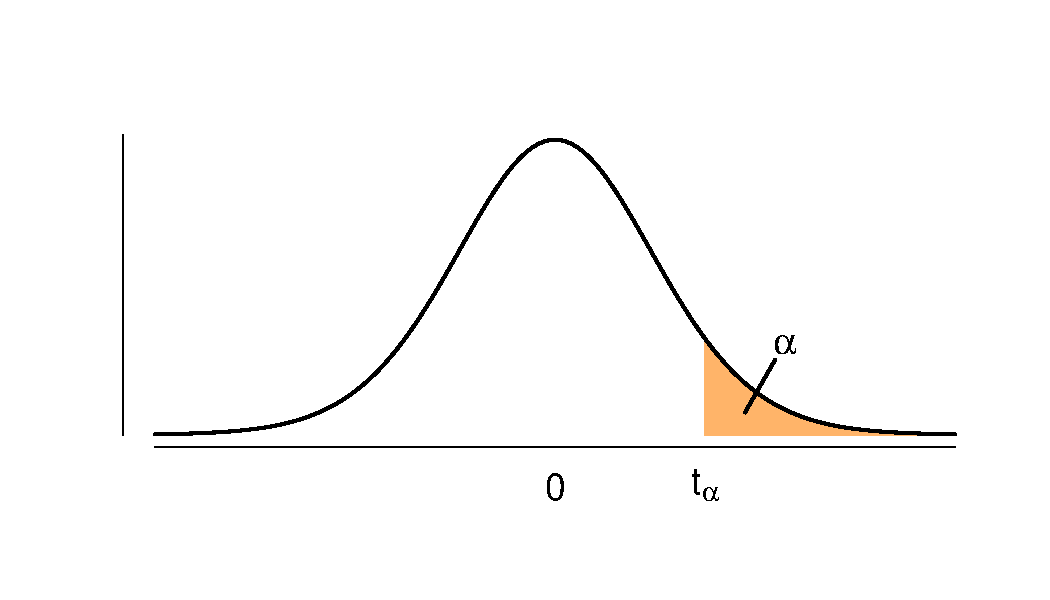
\includegraphics[width=\textwidth]{Files/Images/tdist.pdf}
\end{minipage}

\begin{center}
\small
\begin{tabular}{c|c|c|c|c|c|c|c}
\hline
\multicolumn{1}{c}{$df_{n-1}$} & \multicolumn{1}{c}{$t_{.100}$} & \multicolumn{1}{c}{$t_{.05}$}  & \multicolumn{1}{c}{$t_{.025}$}  & \multicolumn{1}{c}{$t_{.01}$}   & \multicolumn{1}{c}{$t_{.005}$}  & \multicolumn{1}{c}{$t_{.001}$}   & \multicolumn{1}{c}{$t_{.0005}$}  \tstrut\bstrut\\
\hline
\textbf{1}  & 3.078 & 6.314 & 12.706 & 31.821 & 63.657 & 318.309 & 636.619 \tstrut\\
\textbf{2}  & 1.886 & 2.920 & 4.303  & 6.965  & 9.925  & 22.327  & 31.599  \\
\textbf{3}  & 1.638 & 2.353 & 3.182  & 4.541  & 5.841  & 10.215  & 12.924  \\
\textbf{4}  & 1.533 & 2.132 & 2.776  & 3.747  & 4.604  & 7.173   & 8.610   \\
\textbf{5}  & 1.476 & 2.015 & 2.571  & 3.365  & 4.032  & 5.893   & 6.869   \\
\textbf{6}  & 1.440 & 1.943 & 2.447  & 3.143  & 3.707  & 5.208   & 5.959   \\
\textbf{7}  & 1.415 & 1.895 & 2.365  & 2.998  & 3.499  & 4.785   & 5.408   \\
\textbf{8}  & 1.397 & 1.860 & 2.306  & 2.896  & 3.355  & 4.501   & 5.041   \\
\textbf{9}  & 1.383 & 1.833 & 2.262  & 2.821  & 3.250  & 4.297   & 4.781   \\
\textbf{10} & 1.372 & 1.812 & 2.228  & 2.764  & 3.169  & 4.144   & 4.587   \\
\textbf{11} & 1.363 & 1.796 & 2.201  & 2.718  & 3.106  & 4.025   & 4.437   \\
\textbf{12} & 1.356 & 1.782 & 2.179  & 2.681  & 3.055  & 3.930   & 4.318   \\
\textbf{13} & 1.350 & 1.771 & 2.160  & 2.650  & 3.012  & 3.852   & 4.221   \\
\textbf{14} & 1.345 & 1.761 & 2.145  & 2.624  & 2.977  & 3.787   & 4.140   \\
\textbf{15} & 1.341 & 1.753 & 2.131  & 2.602  & 2.947  & 3.733   & 4.073   \\
\textbf{16} & 1.337 & 1.746 & 2.120  & 2.583  & 2.921  & 3.686   & 4.015   \\
\textbf{17} & 1.333 & 1.740 & 2.110  & 2.567  & 2.898  & 3.646   & 3.965   \\
\textbf{18} & 1.330 & 1.734 & 2.101  & 2.552  & 2.878  & 3.610   & 3.922   \\
\textbf{19} & 1.328 & 1.729 & 2.093  & 2.539  & 2.861  & 3.579   & 3.883   \\
\textbf{20} & 1.325 & 1.725 & 2.086  & 2.528  & 2.845  & 3.552   & 3.850   \\
\textbf{21} & 1.323 & 1.721 & 2.080  & 2.518  & 2.831  & 3.527   & 3.819   \\
\textbf{22} & 1.321 & 1.717 & 2.074  & 2.508  & 2.819  & 3.505   & 3.792   \\
\textbf{23} & 1.319 & 1.714 & 2.069  & 2.500  & 2.807  & 3.485   & 3.768   \\
\textbf{24} & 1.318 & 1.711 & 2.064  & 2.492  & 2.797  & 3.467   & 3.745   \\
\textbf{25} & 1.316 & 1.708 & 2.060  & 2.485  & 2.787  & 3.450   & 3.725   \\
\textbf{26} & 1.315 & 1.706 & 2.056  & 2.479  & 2.779  & 3.435   & 3.707   \\
\textbf{27} & 1.314 & 1.703 & 2.052  & 2.473  & 2.771  & 3.421   & 3.690   \\
\textbf{28} & 1.313 & 1.701 & 2.048  & 2.467  & 2.763  & 3.408   & 3.674   \\
\textbf{29} & 1.311 & 1.699 & 2.045  & 2.462  & 2.756  & 3.396   & 3.659   \\
\textbf{30} & 1.310 & 1.697 & 2.042  & 2.457  & 2.750  & 3.385   & 3.646   \\
\textbf{31} & 1.309 & 1.696 & 2.040  & 2.453  & 2.744  & 3.375   & 3.633   \\
\textbf{32} & 1.309 & 1.694 & 2.037  & 2.449  & 2.738  & 3.365   & 3.622   \\
\textbf{33} & 1.308 & 1.692 & 2.035  & 2.445  & 2.733  & 3.356   & 3.611   \\
\textbf{34} & 1.307 & 1.691 & 2.032  & 2.441  & 2.728  & 3.348   & 3.601   \\
\textbf{35} & 1.306 & 1.690 & 2.030  & 2.438  & 2.724  & 3.340   & 3.591   \\
\textbf{36} & 1.306 & 1.688 & 2.028  & 2.434  & 2.719  & 3.333   & 3.582   \\
\textbf{37} & 1.305 & 1.687 & 2.026  & 2.431  & 2.715  & 3.326   & 3.574   \\
\textbf{38} & 1.304 & 1.686 & 2.024  & 2.429  & 2.712  & 3.319   & 3.566   \\
\textbf{39} & 1.304 & 1.685 & 2.023  & 2.426  & 2.708  & 3.313   & 3.558   \\
\textbf{40} & 1.303 & 1.684 & 2.021  & 2.423  & 2.704  & 3.307   & 3.551  \bstrut\\
\hline
\end{tabular}
\end{center}                      \clearpage
\subsection{Table 4: $X^2$ - values for significance level $\alpha$}
\label{table4}

\vspace*{-30pt}
\begin{minipage}{0.6\textwidth}
\hfill
\end{minipage}
\begin{minipage}{0.4\textwidth}
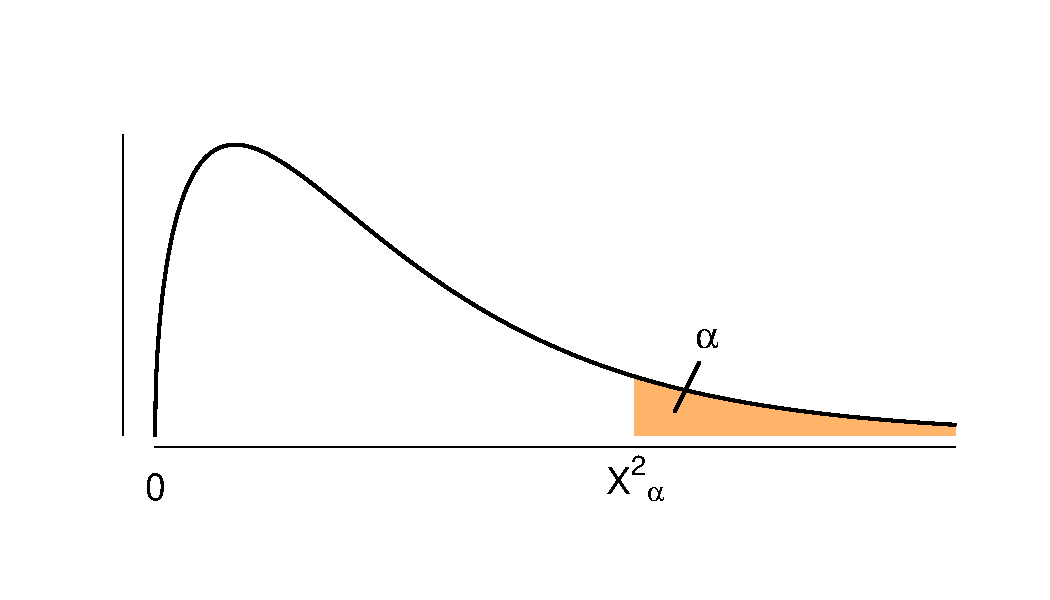
\includegraphics[width=\textwidth]{Files/Images/chisquare.pdf}
\end{minipage}

\begin{center}
\small
\begin{tabular}{c|c|c|c|c|c}
\hline
\multicolumn{1}{c}{$df$} & \multicolumn{1}{c}{$X^2_{.100}$} & \multicolumn{1}{c}{$X^2_{.05}$}  & \multicolumn{1}{c}{$X^2_{.025}$}  & \multicolumn{1}{c}{$X^2_{.01}$}   & \multicolumn{1}{c}{$X^2_{.001}$}   \tstrut\bstrut\\
\hline
\textbf{1}  & 2.706  & 3.841  & 5.024  & 6.635  & 10.828 \tstrut\\
\textbf{2}  & 4.605  & 5.991  & 7.378  & 9.210  & 13.816 \\
\textbf{3}  & 6.251  & 7.815  & 9.348  & 11.345 & 16.266 \\
\textbf{4}  & 7.779  & 9.488  & 11.143 & 13.277 & 18.467 \\
\textbf{5}  & 9.236  & 11.070 & 12.833 & 15.086 & 20.515 \\
\textbf{6}  & 10.645 & 12.592 & 14.449 & 16.812 & 22.458 \\
\textbf{7}  & 12.017 & 14.067 & 16.013 & 18.475 & 24.322 \\
\textbf{8 } & 13.362 & 15.507 & 17.535 & 20.090 & 26.125 \\
\textbf{9}  & 14.684 & 16.919 & 19.023 & 21.666 & 27.877 \\
\textbf{10} & 15.987 & 18.307 & 20.483 & 23.209 & 29.588 \\
\textbf{11} & 17.275 & 19.675 & 21.920 & 24.725 & 31.264 \\
\textbf{12} & 18.549 & 21.026 & 23.337 & 26.217 & 32.910 \\
\textbf{13} & 19.812 & 22.362 & 24.736 & 27.688 & 34.528 \\
\textbf{14} & 21.064 & 23.685 & 26.119 & 29.141 & 36.123 \\
\textbf{15} & 22.307 & 24.996 & 27.488 & 30.578 & 37.697 \\
\textbf{16 }& 23.542 & 26.296 & 28.845 & 32.000 & 39.252 \\
\textbf{17} & 24.769 & 27.587 & 30.191 & 33.409 & 40.790 \\
\textbf{18} & 25.989 & 28.869 & 31.526 & 34.805 & 42.312 \\
\textbf{19} & 27.204 & 30.144 & 32.852 & 36.191 & 43.820 \\
\textbf{20} & 28.412 & 31.410 & 34.170 & 37.566 & 45.315 \\
\textbf{21} & 29.615 & 32.671 & 35.479 & 38.932 & 46.797 \\
\textbf{22} & 30.813 & 33.924 & 36.781 & 40.289 & 48.268 \\
\textbf{23} & 32.007 & 35.172 & 38.076 & 41.638 & 49.728 \\
\textbf{24} & 33.196 & 36.415 & 39.364 & 42.980 & 51.179 \\
\textbf{25} & 34.382 & 37.652 & 40.646 & 44.314 & 52.620 \\
\textbf{26} & 35.563 & 38.885 & 41.923 & 45.642 & 54.052 \\
\textbf{27} & 36.741 & 40.113 & 43.195 & 46.963 & 55.476 \\
\textbf{28} & 37.916 & 41.337 & 44.461 & 48.278 & 56.892 \\
\textbf{29} & 39.087 & 42.557 & 45.722 & 49.588 & 58.301 \\
\textbf{30} & 40.256 & 43.773 & 46.979 & 50.892 & 59.703 \\
\textbf{31} & 41.422 & 44.985 & 48.232 & 52.191 & 61.098 \\
\textbf{32} & 42.585 & 46.194 & 49.480 & 53.486 & 62.487 \\
\textbf{33} & 43.745 & 47.400 & 50.725 & 54.776 & 63.870 \\
\textbf{34} & 44.903 & 48.602 & 51.966 & 56.061 & 65.247 \\
\textbf{35} & 46.059 & 49.802 & 53.203 & 57.342 & 66.619 \\
\textbf{36} & 47.212 & 50.998 & 54.437 & 58.619 & 67.985 \\
\textbf{37} & 48.363 & 52.192 & 55.668 & 59.893 & 69.347 \\
\textbf{38} & 49.513 & 53.384 & 56.896 & 61.162 & 70.703 \\
\textbf{39} & 50.660 & 54.572 & 58.120 & 62.428 & 72.055 \\
\textbf{40} & 51.805 & 55.758 & 59.342 & 63.691 & 73.402 \bstrut\\
\hline
\end{tabular}
\end{center}                      \clearpage
\subsection{Table 5: F - values for significance level 0.05}
\label{table5}

\vspace*{-30pt}
\begin{minipage}{0.6\textwidth}
\hfill
\end{minipage}
\begin{minipage}{0.4\textwidth}
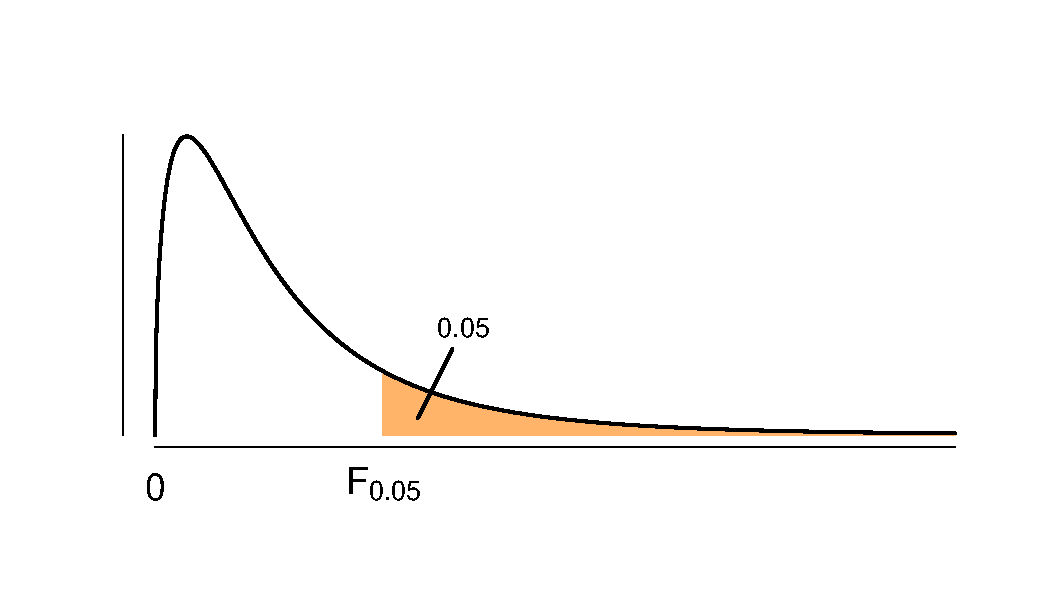
\includegraphics[width=\textwidth]{Files/Images/fdist.pdf}
\end{minipage}

\begin{center}
\small
\begin{tabular}{c|c|c|c|c|c|c|c|c|c}
\hline
\multicolumn{1}{c}{\textbf{$_{df_R} { }^{df_M}$}}  & \multicolumn{1}{c}{\textbf{1}} & \multicolumn{1}{c}{\textbf{2}} & \multicolumn{1}{c}{\textbf{3}} & \multicolumn{1}{c}{\textbf{4}} & \multicolumn{1}{c}{\textbf{5}} & \multicolumn{1}{c}{\textbf{6}} & \multicolumn{1}{c}{\textbf{7}} & \multicolumn{1}{c}{\textbf{8}} & \multicolumn{1}{c}{\textbf{9}} \tstrut\bstrut\\
\hline
\textbf{1}   & 161.4476   & 199.5000   & 215.7073   & 224.5832   & 230.1619   & 233.9860   & 236.7684   & 238.8827   & 240.5433      \tstrut\\
\textbf{2}   & 18.5128    & 19.0000    & 19.1643    & 19.2468    & 19.2964    & 19.3295    & 19.3532    & 19.3710    & 19.3848       \\
\textbf{3}   & 10.1280    & 9.5521     & 9.2766     & 9.1172     & 9.0135     & 8.9406     & 8.8867     & 8.8452     & 8.8123        \\
\textbf{4}   & 7.7086     & 6.9443     & 6.5914     & 6.3882     & 6.2561     & 6.1631     & 6.0942     & 6.0410     & 5.9988          \\
\textbf{5}   & 6.6079     & 5.7861     & 5.4095     & 5.1922     & 5.0503     & 4.9503     & 4.8759     & 4.8183     & 4.7725          \\
\textbf{6}   & 5.9874     & 5.1433     & 4.7571     & 4.5337     & 4.3874     & 4.2839     & 4.2067     & 4.1468     & 4.0990         \\
\textbf{7}   & 5.5914     & 4.7374     & 4.3468     & 4.1203     & 3.9715     & 3.8660     & 3.7870     & 3.7257     & 3.6767           \\
\textbf{8}   & 5.3177     & 4.4590     & 4.0662     & 3.8379     & 3.6875     & 3.5806     & 3.5005     & 3.4381     & 3.3881         \\
\textbf{9}   & 5.1174     & 4.2565     & 3.8625     & 3.6331     & 3.4817     & 3.3738     & 3.2927     & 3.2296     & 3.1789         \\
\textbf{10}  & 4.9646     & 4.1028     & 3.7083     & 3.4780     & 3.3258     & 3.2172     & 3.1355     & 3.0717     & 3.0204          \\
\textbf{11}  & 4.8443     & 3.9823     & 3.5874     & 3.3567     & 3.2039     & 3.0946     & 3.0123     & 2.9480     & 2.8962        \\
\textbf{12}  & 4.7472     & 3.8853     & 3.4903     & 3.2592     & 3.1059     & 2.9961     & 2.9134     & 2.8486     & 2.7964         \\
\textbf{13}  & 4.6672     & 3.8056     & 3.4105     & 3.1791     & 3.0254     & 2.9153     & 2.8321     & 2.7669     & 2.7144         \\
\textbf{14}  & 4.6001     & 3.7389     & 3.3439     & 3.1122     & 2.9582     & 2.8477     & 2.7642     & 2.6987     & 2.6458          \\
\textbf{15}  & 4.5431     & 3.6823     & 3.2874     & 3.0556     & 2.9013     & 2.7905     & 2.7066     & 2.6408     & 2.5876         \\
\textbf{16}  & 4.4940     & 3.6337     & 3.2389     & 3.0069     & 2.8524     & 2.7413     & 2.6572     & 2.5911     & 2.5377     \\
\textbf{17}  & 4.4513     & 3.5915     & 3.1968     & 2.9647     & 2.8100     & 2.6987     & 2.6143     & 2.5480     & 2.4943          \\
\textbf{18}  & 4.4139     & 3.5546     & 3.1599     & 2.9277     & 2.7729     & 2.6613     & 2.5767     & 2.5102     & 2.4563         \\
\textbf{19}  & 4.3807     & 3.5219     & 3.1274     & 2.8951     & 2.7401     & 2.6283     & 2.5435     & 2.4768     & 2.4227           \\
\textbf{20}  & 4.3512     & 3.4928     & 3.0984     & 2.8661     & 2.7109     & 2.5990     & 2.5140     & 2.4471     & 2.3928           \\
\textbf{21}  & 4.3248     & 3.4668     & 3.0725     & 2.8401     & 2.6848     & 2.5727     & 2.4876     & 2.4205     & 2.3660           \\
\textbf{22}  & 4.3009     & 3.4434     & 3.0491     & 2.8167     & 2.6613     & 2.5491     & 2.4638     & 2.3965     & 2.3419          \\
\textbf{23}  & 4.2793     & 3.4221     & 3.0280     & 2.7955     & 2.6400     & 2.5277     & 2.4422     & 2.3748     & 2.3201          \\
\textbf{24}  & 4.2597     & 3.4028     & 3.0088     & 2.7763     & 2.6207     & 2.5082     & 2.4226     & 2.3551     & 2.3002          \\
\textbf{25}  & 4.2417     & 3.3852     & 2.9912     & 2.7587     & 2.6030     & 2.4904     & 2.4047     & 2.3371     & 2.2821         \\
\textbf{26}  & 4.2252     & 3.3690     & 2.9752     & 2.7426     & 2.5868     & 2.4741     & 2.3883     & 2.3205     & 2.2655          \\
\textbf{27}  & 4.2100     & 3.3541     & 2.9604     & 2.7278     & 2.5719     & 2.4591     & 2.3732     & 2.3053     & 2.2501          \\
\textbf{28}  & 4.1960     & 3.3404     & 2.9467     & 2.7141     & 2.5581     & 2.4453     & 2.3593     & 2.2913     & 2.2360           \\
\textbf{29}  & 4.1830     & 3.3277     & 2.9340     & 2.7014     & 2.5454     & 2.4324     & 2.3463     & 2.2783     & 2.2229          \\
\textbf{30}  & 4.1709     & 3.3158     & 2.9223     & 2.6896     & 2.5336     & 2.4205     & 2.3343     & 2.2662     & 2.2107        \\
\textbf{40}  & 4.0847     & 3.2317     & 2.8387     & 2.6060     & 2.4495     & 2.3359     & 2.2490     & 2.1802     & 2.1240         \\
\textbf{60}  & 4.0012     & 3.1504     & 2.7581     & 2.5252     & 2.3683     & 2.2541     & 2.1665     & 2.0970     & 2.0401       \\
\textbf{120} & 3.9201     & 3.0718     & 2.6802     & 2.4472     & 2.2899     & 2.1750     & 2.0868     & 2.0164     & 1.9588        \\
\textbf{$\infty$}   & 3.8415     & 2.9957     & 2.6049     & 2.3719     & 2.2141     & 2.0986     & 2.0096     & 1.9384     & 1.8799     \bstrut \\
\hline
\end{tabular}
\end{center}                      \clearpage

% R Help
\addtocontents{toc}{\protect\vspace{10pt}}
\section{R help}
\label{rhelp}

\subsection{Part I: Basic functionality}

\textit{1.1 Types of data} \\
\\
\begin{minipage}[t]{.4\textwidth}
\vspace*{-8pt}
\rcode{numeric} \\
\rcode{character} \\
\rcode{logical} \\
\rcode{factor} \\ 			
\rcode{Inf} \\					
\rcode{NaN} \\ 					 
\rcode{NA}  
\end{minipage}
\begin{minipage}[t]{.6\textwidth}
Numbers \\
Words (text) \\
TRUE or FALSE \\
One of the above with predefined categories \\
Infinite \\
Not a number \\
Not available
\end{minipage}
\vspace*{.5cm}

\textit{1.2 Assigning values to variables} \\
\\
There are multiple ways to assign a value to a variable. For example, these all do the same, which is assigning the value \rcode{1} to the variable \rcode{a}.\\
\\
\begin{center}
    \rcode{a = 1} or \rcode{a <- 1} \hspace{2.5cm} \rcode{assign(\textquotesingle a\textquotesingle, 1)}  \hspace{2.5cm}	\rcode{a = b = 1} 
\end{center}
\vspace*{0.5cm}
\textit{1.3 Data structures} \\
\\
\begin{minipage}[t]{.4\textwidth}
\vspace*{-8pt}
\rcode{vector} \\ 				 
\rcode{matrix} \\				
\rcode{array} 	\\			
\rcode{data frame} \\				 
\rcode{list} 				
\end{minipage}
\begin{minipage}[t]{.6\textwidth}
A one-dimensional data structure \\
A two-dimensional data structure \\
A multi-dimensional data structure \\
A data structure containing different types of data \\
A collection of different data structures
\end{minipage}
\vspace*{.5cm}

\textit{1.4 Vectors} \\
\\
\begin{minipage}[t]{.4\textwidth}
\vspace*{-8pt}
\rcode{c(1, 2, 3)} \\			 
\rcode{seq(1, 6, 2) } \\			
\rcode{rep(1:3, 2)} \\				
\rcode{1:4} \\ 					
\rcode{paste(x, y)} \\ 				 
\rcode{letters[1:5]} \\ 			
\rcode{sample(x, 5)} \\ 			 
\rcode{length(x) } \\				
\rcode{cut(x, 5)} \\ 				
\rcode{append(x, c(4, 5))} \\ 		
\rcode{x <- numeric()} \\ 			
\rcode{sort(x) 	} \\			
\end{minipage}
\begin{minipage}[t]{.6\textwidth}
Combine the numbers 1, 2, and 3 in a vector \\
Create sequence from 1 to 6 in increments of 2 \\
Repeat 1 to 3, and do that 2 times \\
Vector of 1 t/m 4 (\rcode{:} is therefore making a vector) \\
Paste vectors \rcode{x} and y together \\
Vector of first 5 letters of the alphabet  \\
Gives a random sample of size 5 from of data \rcode{x} \\
Indicates the length of \rcode{x} \\
Divide \rcode{x} in vectors with length 5 \\
Add the numbers 4 and 5 to vector \rcode{x} \\
Creates an empty vector \rcode{x} \\
Order vector \rcode{x} from low to high (default) \\
\end{minipage}
\vspace*{.5cm}

\clearpage % Page break

\textit{1.5 Matrices} \\
\\
\begin{minipage}[t]{.4\textwidth}
\vspace*{-8pt}
\rcode{matrix(1:9, 3, 3) } \\			
\rcode{diag(x) 		} \\		
\rcode{head(x, 2) } \\				
\rcode{t(x) 	} \\			
\rcode{rbind(x, y) 	} \\		
\rcode{cbind(x, y) 	} \\		
\end{minipage}
\begin{minipage}[t]{.6\textwidth}
Create a matrix of 1 t/m 9 with 3 rows and 3 columns  \\
Get the diagonal from matrix \rcode{x} \\
Gives the first two rows of matrix or data frame \rcode{x} \\
Gives transpose of matrix \rcode{x} \\
Add rows from matrix \rcode{x} and \rcode{y} together \\
Add columns from matrix \rcode{x} and \rcode{y} together \\
\end{minipage}
\vspace*{.5cm}

\textit{1.6 Data frames} \\
\\
\begin{minipage}[t]{.4\textwidth}
\vspace*{-8pt}
\rcode{data.frame(\textquotesingle X\textquotesingle = x) } \\
\rcode{head(x, 2) 	} \\			
\rcode{names(x) } \\				
\rcode{colnames(x) 	} \\			
\rcode{rownames(x) 	} \\
\end{minipage}
\begin{minipage}[t]{.6\textwidth}
Create a data frame with data \rcode{x} (\rcode{X} is the column name) \\
Look at first two rows of data frame \rcode{x} \\
Names of data frame \rcode{x} \\
Column names of data frame \rcode{x} \\
Row names of data frame \rcode{x} \\
\end{minipage}
\vspace*{.5cm}

\textit{1.7 Lists} \\
\\
\begin{minipage}[t]{.4\textwidth}
\vspace*{-8pt}
\rcode{x <- list()} \\ 				
\rcode{x[[\textquotesingle title\textquotesingle]] <- m} \\	
\end{minipage}
\begin{minipage}[t]{.6\textwidth}
Create an empty list \rcode{x}  \\
Insert structure \rcode{m} into list \rcode{x} (\rcode{title} is the new title)
\end{minipage}
\vspace*{.5cm}

\textit{1.8 Indexing} \\
\\
\begin{minipage}[t]{.4\textwidth}
\vspace*{-8pt}
\rcode{x[2] 	} \\				
\rcode{x[1:5] 	} \\			
\rcode{x[-1] 	} \\			
\rcode{x[x > 5] } \\				
\rcode{x[x > 3 \& x < 6] } \\			 
\rcode{x[1:3, 1] 	} \\		
\rcode{x[1:3, 1:4] 	} \\
\rcode{x\$h or x[\textquotesingle h\textquotesingle]	}	
\end{minipage}
\begin{minipage}[t]{.6\textwidth}
Get the second element from the vector \rcode{x} \\
Get the first to the fifth element from vector \rcode{x} \\
Get all elements except first element from vector \rcode{x} \\
Get all elements greater than 5 from vector \rcode{x} \\
Get all values from \rcode{x} greater than 3 and less than 6 \\
Get first 3 values from the first column from data \rcode{x} \\
Get first 3 values from the first four columns from \rcode{x} \\
Select element \rcode{h} from data frame \rcode{x}
\end{minipage}
\vspace*{.5cm}

\textit{1.9 Operators} \\
\\
\begin{minipage}[t]{.4\textwidth}
\vspace*{-8pt}
\rcode{x == y 	} \\			
\rcode{x != y } \\				
\rcode{\%\% } 	
\end{minipage}
\begin{minipage}[t]{.6\textwidth}
Check if \rcode{x} equals \rcode{y} \\
Check if \rcode{x} does not equal \rcode{y} \\
The remainder of a division (e.g. \rcode{36\%\%5} = 1)	
\end{minipage}
\vspace*{.5cm}

\textit{1.10 Importing data and files} \\
\\
\begin{minipage}[t]{.4\textwidth}
\vspace*{-8pt}
\rcode{data(\textquotesingle x\textquotesingle)} \\ 				
\rcode{file.choose() } \\ 			
\rcode{read.table(\textquotesingle x\textquotesingle)} \\  			
\rcode{write.table(x) } \\ 		
\rcode{read.csv(\textquotesingle x\textquotesingle) } \\ 		
\rcode{write.csv(x) } \\ 		
\end{minipage}
\begin{minipage}[t]{.6\textwidth}
Import data set \rcode{x} \\
Get access to interface to select a file \\
Read in a \dataset{.txt} file \rcode{x} from the working directory \\
Writes data \rcode{x} to a \dataset{.txt} file from the working directory \\
Reads in a \dataset{.csv} file \rcode{x} from the working directory \\
Writes data \rcode{x} to a \dataset{.csv} file from the working directory 
\end{minipage}
\vspace*{.5cm}

\clearpage % Page break

\textit{1.11 Basic functions} \\
\\
\begin{minipage}[t]{.4\textwidth}
\vspace*{-8pt}
\rcode{TAB} \\ 					
\rcode{ls() } \\ 					 
\rcode{rm(list = ls())} \\  		
\rcode{getwd()	} \\ 	 		
\rcode{setwd() 	} \\ 		
\rcode{help(x) 	} \\ 
\rcode{str(x)	 } \\ 		
\rcode{summary(x) 	} \\ 			
\rcode{print(\textquotesingle Hello\textquotesingle) } \\ 		
\rcode{round(x, digits = 2)} \\  		  
\rcode{which.max(x) } \\ 			 
\rcode{which(x == 10) 	} \\ 	
\rcode{unique(x)	} \\ 		
\rcode{length(x)	} \\ 		
\rcode{nrow(x)	} \\ 		
\rcode{ncol(x)	} \\ 				
\end{minipage}
\begin{minipage}[t]{.6\textwidth}
Scrolling through functions beginning with that letter  \\
See all variables available in the environment \\
Delete all variables in your environment \\
See the location of your working directory  \\
Set the location of your working directory  \\
Read help about the function \rcode{x} \\
Finds out the structure of data \rcode{x}  \\
Gives summary of the object \rcode{x} \\
Print \rcode{Hello} to the output \\
Round number(s) in \rcode{x} to a specified number of digits \\
Indicates the place of the highest value of data \rcode{x} \\
Shows the place of each object in \rcode{x} that equals 10 \\
Gives only the unique values in \rcode{x} \\
Gives the number of elements in \rcode{x} \\
Gives number of rows of matrix/data frame \rcode{x} \\
Gives number of columns of matrix/data frame \rcode{x}
\end{minipage}
\vspace*{.5cm}

\textit{1.12 Installing an add-on package} \\
\\
\begin{minipage}[t]{.4\textwidth}
\vspace*{-8pt}
\rcode{install.packages(\textquotesingle x\textquotesingle)}		
\end{minipage}
\begin{minipage}[t]{.6\textwidth}
Installs package with name \rcode{x} 	
\end{minipage}
\vspace*{.5cm}

\clearpage % Page break                                         \clearpage
\subsection{Part II: Commands for creating graphics}

\textit{2.1 Creating a plot} \\
\\
\begin{minipage}[t]{.4\textwidth}
\vspace*{-8pt}
\rcode{plot(x, y, ...) } \\
\\
\\
\rcode{points(x, y) } \\
\rcode{lines(x, y) } \\
\rcode{abline() 	} \\
\rcode{text(x, y, \textquotesingle text\textquotesingle) } \\
\rcode{legend(\textquotesingle bottomright\textquotesingle) } \\
\\
\rcode{pdf(\textquotesingle x\textquotesingle) 	} \\		
\rcode{dev.off() 	} \\
\rcode{layout(matrix(1:6, 2, 3)) } \\
\rcode{layout(1) 	} \\
\rcode{curve(dnorm(x, 0, 1), -3, 3)} \\
\end{minipage}
\begin{minipage}[t]{.6\textwidth}
The basic plot function. Can be extended by adding arguments in \rcode{...} \\
\\
Adds points with \rcode{x} and \rcode{y} values to an existing plot \\
Adds a line with \rcode{x} and \rcode{y} values to an existing plot \\
Adds a linear line to plot (see \rcode{?abline}) \\
Add text to plot on \rcode{x} and \rcode{y} coordinates \\
Inserts legend in the bottom right of the plot \\
\\
When called, writes all images to \dataset{.pdf} file \rcode{x} \\
Ends writing all created images to a file  \\
Create the layout (for multiple figures) \\
Put every plot on one page \\
Plot the curve of the standard normal distribution
\end{minipage}
\vspace*{.5cm}

\textit{2.2 Quick plot functions} \\
\\
\begin{minipage}[t]{.4\textwidth}
\vspace*{-8pt}
\rcode{hist(x, ...) } \\
\rcode{dotchart(x, ...) } \\
\rcode{pairs(x, ...) } \\	 
\rcode{boxplot(x, ...) } \\
\rcode{barplot(x, ...)	}
\end{minipage}
\begin{minipage}[t]{.6\textwidth}
Creates a histogram of \rcode{x} \\
Creates a point chart of \rcode{x} \\
Compares all variables of \rcode{x} with multiple plots \\
Creates a box plot of \rcode{x} \\
Creates a bar plot of \rcode{x}
\end{minipage}
\vspace*{.5cm}

\textit{2.3 Additional plot arguments (to be entered in \rcode{...})} \\
\\
\begin{minipage}[t]{.4\textwidth}
\vspace*{-8pt}
\rcode{axes = FALSE} \\ 
\rcode{add = TRUE} \\ 
\rcode{las = 1} \\ 
\rcode{xlim = c(0, 1)} \\ 	
\rcode{ylim = c(0, 1) } \\ 
\rcode{xlab = \textquotesingle x-axis\textquotesingle} \\ 
\rcode{ylab = \textquotesingle y-axis\textquotesingle} \\ 
\rcode{type = \textquotesingle p\textquotesingle} \\ 
\rcode{type = \textquotesingle l\textquotesingle} \\ 
\rcode{type = \textquotesingle b\textquotesingle} \\ 
\rcode{lty = 1} \\ 
\rcode{col = \textquotesingle blue\textquotesingle} 
\end{minipage}
\begin{minipage}[t]{.6\textwidth}
Disable axis in plot \\
Adds the created plot to the previous plot  \\
Rotates the labels on the \rcode{x} and \rcode{y} axes \\
Set the range of the \rcode{x} axis between 0 and 1 \\
Set the range of the \rcode{y} axis between 0 and 1 \\
Set the name of the \rcode{x} axis to \rcode{x-axis} \\
Set the name of the \rcode{y} axis to \rcode{y-axis} \\
Creates a plot containing the data as points \\
Creates a plot containing the data as line \\
Creates both points and lines \\
Set the line type in the plot \\
Set the color in the plot to \rcode{blue}
\end{minipage}
\vspace*{.5cm}

\clearpage % Page break                                         \clearpage
\subsection{Part III: If-statements, loops, and functions}

\textit{3.1 If-statements} \\
\\
\rcode{If}-statements have the following structure: \\

\codeblock{if (condition)\{ \\
  \hspace*{20pt}{\color{dataset}\# Perform an action} \\
\}
}

\begin{minipage}[t]{0.2\textwidth}
Translation:
\end{minipage}
\begin{minipage}[t]{0.8\textwidth}
If this \rcode{condition} is satisfied, then perform this action.
\end{minipage} \\
\\
Note that \rcode{length(condition) == 1} must evaluate to \rcode{TRUE}. \\
\\ 
\textit{3.2 If-else-statements} \\
\\
\rcode{If-else}-statements have the following structure: \\

\codeblock{if (condition)\{ \\
  \hspace*{20pt}{\color{dataset}\# Perform an action} \\
\} else \{ \\
\hspace*{20pt}{\color{dataset}\# Perform a different action} \\
\}
}

\begin{minipage}[t]{0.2\textwidth}
Translation:
\end{minipage}
\begin{minipage}[t]{0.8\textwidth}
If this \rcode{condition} is satisfied, then perform this action. If this condition is not satisfied, then perform a different action.
\end{minipage} \\
\\
Another \rcode{condition} can be added by putting another \rcode{if (condition)} after \rcode{else}. \\

\codeblock{if (condition)\{ \\
  \hspace*{20pt}{\color{dataset}\# Perform an action} \\
\} else if (other condition)\{ \\
\hspace*{20pt}{\color{dataset}\# Perform a different action} \\
\}
}

\begin{minipage}[t]{0.2\textwidth}
Translation:
\end{minipage}
\begin{minipage}[t]{0.8\textwidth}
If this \rcode{condition} is satisfied, then perform this action. If not, then check whether the \rcode{other condition} is satisfied. If the \rcode{other condition} is	satisfied, perform a different action. 
\end{minipage} \\
\\
\clearpage % Page break

\textit{3.3 For-loops} \\
\\
\rcode{for}-loops have the following structure: \\

\codeblock{for(i in 1:4)\{ \\
  \hspace*{20pt}{\color{dataset}\# Perform an action that needs to repeated } \\
\}
}

\begin{minipage}[t]{0.2\textwidth}
Translation:
\end{minipage}
\begin{minipage}[t]{0.8\textwidth}
For a specified number of times (\rcode{1:4}), perform this action on each iteration (\rcode{i}).
\end{minipage} \\
\\

\textit{3.4 While-loops} \\
\\
\rcode{while}-loops have the following structure: \\

\codeblock{while(condition)\{ \\
  \hspace*{20pt}{\color{dataset}\# Perform an action that needs to be repeated} \\
\}
}

\begin{minipage}[t]{0.2\textwidth}
Translation:
\end{minipage}
\begin{minipage}[t]{0.8\textwidth}
For an unspecified number of times, perform this action as long as the \rcode{condition} is \rcode{TRUE}.
\end{minipage} \\
\\

\textit{3.5 Functions} \\
\\
Functions have the following structure: \\

\codeblock{myFunction <- function(x, ...)\{ \\
  \\
  \hspace*{20pt}{\color{dataset}\# Perform action on input x to get result } \\
\\
  \hspace*{20pt}return(result) \\
\}

}

\begin{minipage}[t]{0.2\textwidth}
Translation:
\end{minipage}
\begin{minipage}[t]{0.8\textwidth}
Take the input \rcode{x}, perform some actions, and return the resulting \rcode{outcome}.
\end{minipage} \\
\\
The function \rcode{myFunction} can then be called with the data in \rcode{x} using: \\
\\
\codeblock{myFunction(x)}

\clearpage % Page break                                         \clearpage
\subsection{Part IV: Descriptive statistics and hypothesis testing}

\textit{4.1 Descriptive statistics} \\
\\
\begin{minipage}[t]{.4\textwidth}
\vspace*{-8pt}
\rcode{mean(x) } \\ 
\rcode{median(x) } \\
\rcode{sum(x) } \\
\rcode{min(x) } \\ 
\rcode{max(x) } \\	
\rcode{sd(x)  } \\
\rcode{var(x) } \\
\rcode{cor(x, y) } \\
\rcode{table(x) } \\
\end{minipage}
\begin{minipage}[t]{.6\textwidth}
Gives the \concept{average} of \rcode{x} \\
Gives the \concept{median} of \rcode{x} \\
Gives the \concept{sum} of \rcode{x} \\
Gives the \concept{minimum} of \rcode{x} \\
Gives the \concept{maximum} of \rcode{x} \\
Gives the \concept{standard deviation} of \rcode{x} \\
Gives the \concept{variance} of \rcode{x} \\
Gives the \concept{correlation} between \rcode{x} and \rcode{y} \\
Gives a \concept{frequency table} of \rcode{x}  \\
\end{minipage}
\vspace*{.5cm}

\textit{4.2 Simple hypothesis testing} \\
\\
\begin{minipage}[t]{.4\textwidth}
\vspace*{-8pt}
\rcode{t.test(x, y) } \\
\rcode{cor.test(x, y) } \\	
\rcode{binom.test(x, n, p)} \\
\rcode{chisq.test(x, y)} \\
\rcode{aov(formula, x) 	} \\	
\end{minipage}
\begin{minipage}[t]{.6\textwidth}
Performs a \concept{t-test} on the data \rcode{x} (\rcode{y} is optional) \\
Performs a \concept{correlation test} on the data \rcode{x} and \rcode{y} \\
Performs a \concept{binomial test} on the data \\
Performs a \concept{chi-square test} on the data \\
Performs an \concept{ANOVA} on the data in \rcode{x} using formula \\
\end{minipage}
\vspace*{.5cm}

\textit{4.3 Regression} \\
\\
\begin{minipage}[t]{.4\textwidth}
\vspace*{-8pt}
\rcode{lm(y {\raise.17ex\hbox{$\scriptstyle\sim$}} 1 + x) } \\	
\rcode{lm(y {\raise.17ex\hbox{$\scriptstyle\sim$}} 1 + x + z) } \\	
\rcode{lm(y {\raise.17ex\hbox{$\scriptstyle\sim$}} 0 + x) } \\
\rcode{lm(y {\raise.17ex\hbox{$\scriptstyle\sim$}} x:z) } \\
\rcode{lm(y {\raise.17ex\hbox{$\scriptstyle\sim$}} x * z) } \\
\rcode{lm(y {\raise.17ex\hbox{$\scriptstyle\sim$}} poly(x, 2)) } \\
\\
\rcode{coef(x) } \\ 
\rcode{residuals(x) } \\  
\rcode{AIC(x) } \\
\rcode{BIC(x)  } \\
\rcode{summary(x) } \\
\rcode{confint(x) 	 } \\
\rcode{abline(x)} \\
\rcode{predict(x, newdata)} \\
\end{minipage}
\begin{minipage}[t]{.6\textwidth}
Regression model $y = \beta_0 + \beta_1 \times x$  \\
Regression model $y = \beta_0 + \beta_1 \times x + \beta_2 \times z$  \\
Regression model $y = \beta_1 \times x$  \\
Regression model $y = \beta_0 + \beta_1 \times x \times z$ \\ 
Regression model $y = \beta_0 + \beta_1 \times x + \beta_2 \times z + \beta_3 \times x \times z$ \\
Regression model $y = \beta_0 + \beta_1 \times x^2$ \\
\\
Gives \concept{coefficients} of regression model in \rcode{x} \\
Gives \concept{residuals} of regression model in \rcode{x} \\
Gives the \concept{AIC} value of regression model in \rcode{x}  \\
Gives the \concept{BIC} value of regression model in \rcode{x} \\
Gives a summary of \concept{regression model} in \rcode{x}  \\
Gives the \concept{confidence interval} of model \rcode{x} \\
When added to a plot, plots the regression line \\
Use the \concept{regression model} in \rcode{x} to predict new data \\
\end{minipage}
\vspace*{.5cm}

\clearpage % Page break                                         \clearpage

% R exercises
\addtocontents{toc}{\protect\vspace{10pt}}
\section{Beginner R exercises}

\subsection{Creating and removing objects in the environment}

\question{
    B 1
}{
    Run the following code in \texttt{R}: \\
    
    \codeblock{a = b = 1\\
a = 2}

What happened? How do you know (which command)? How many objects did you create in your environment? Try assigning the values using the \rcode{<-} operator. Does the result differ from the result when you are using \rcode{=} to create the variables? 
}   

\question{
B 2
}{
Remove the variables\rcode{a} and \rcode{b} from your environment using the \rcode{rm()} function.
}

\question{
B 3
}{
Run the following code in \texttt{R}: \\
\\
\codeblock{apple <- banana <- lemon <- 1}
Remove all objects with an 'n' in the name.
}

\question{
B 4
}{
Run the following code in \texttt{R}: \\
\\
\codeblock{apples <- 5; pears <- 3; pineapples <- 6}
Then try the following code: \\
\\
\codeblock{apples + pineapples \\
apples + Pears
}
Why can't you add \rcode{apples} and \rcode{Pears}?
}

\question{
B 5
}{
Use \texttt{R} to compute the square root of 81 and store the result in \rcode{t1}. 
}

\question{
B 6
}{
Use \texttt{R} to compute 81 to the power a half and store the result in \rcode{t2}. 
}

\question{
B 7
}{
Use the \rcode{==} operator to check whether the contents of \rcode{t1} and \rcode{t2} are the same.
}

\clearpage % Page break
\subsection{Working directory and help functionality}

\question{
B 8
}{
With the command \rcode{getwd()} you can find the current working directory of the \texttt{R} process. Explain what the working directory means and why it is important.
}

\question{
B 9
}{
Change the working directory of the \texttt{R} session to a folder of your preference. What function do you use? How can you check whether your change has worked?
}

\question{
B 10
}{
Run the following code in \texttt{R}: \\
\\
\codeblock{demo(package = .packages(all.available = TRUE))}
What does this code do? How do you run the demo \rcode{persp} (in package \rcode{graphics})?
}

\question{
B 11
}{
Run the following code in \texttt{R}: \\
\\
\codeblock{a <- c(1, 6, 7, 8, 9, NA) \\
mean(a)}
This gives \rcode{NA}, why? Check \rcode{?mean} to find out what arguments the \rcode{mean()} function takes as input. Can you find a way to compute the mean with the missing value removed?
}

\question{
B 12
}{
According to Google there exists an R-function called \rcode{mvrnorm()}. Typing \rcode{mvrnorm} or \rcode{?mvrnorm}, however, gives an error. Why? Which library do you have to load first? How?
}

\question{
B 13
}{
What does \rcode{\%\%} do? Can you ask help with \rcode{?\%\%}, like in \rcode{?mean}? If not, how? What is \rcode{\%\%} doing?
}

\question{
B 14
}{
The \rcode{cor()} function computes correlations. As an example, run the following code in \texttt{R}: \\
\\
\codeblock{cor(c(1, 2, 3, 4), c(1, 4, 7, 15))}
How can you find out (which function) whether this correlation is statistically significant? How can you find such a function? What is the confidence interval of the correlation? How can you find all functions that have 'cor' in their name? 
}

\clearpage
\subsection{Modes of objects}

\question{
B 15
}{
Run the following code in \texttt{R}: \\
\\
\codeblock{a1 <- \textquotesingle 1\textquotesingle; a2 <- 1; a3 <- TRUE}
What are the modes of \rcode{a1}, \rcode{a2}, and \rcode{a3}? Now run the following code in \texttt{R}: \\
\\
\codeblock{b1 <- c(a1, a2); b2 <- c(a1, a3); b3 <- c(a2, a3); b4 <- c(a1, a2, a3)}
What are the modes of \rcode{b1}, \rcode{b2}, \rcode{b3}, and \rcode{b4}? Can you explain?
}

\question{
B 16
}{
Why does \rcode{TRUE/TRUE} yield 1, \rcode{FALSE/TRUE} yield 0, \rcode{FALSE/FALSE} yield \rcode{NaN}, and \rcode{TRUE/FALSE} yields \rcode{Inf}?
}

\question{
B 17
}{
Convert the logical \rcode{TRUE} to a numerical. Convert this numerical to a character. Next, convert the logical \rcode{TRUE} to a character? Why do these results differ? 
}

\question{
B 18  
}{
How can you check whether a vector is numeric? Is the vector \rcode{c(1,0)} a numeric vector? And the vector \rcode{c(TRUE, FALSE)}? And the vector \rcode{c(TRUE, FALSE, 1, 0)}? Why?
}

\clearpage
\subsection{Data types: Vectors}

\question{
B 19 
}{
Use the \rcode{c()} function (or \rcode{:}) to create the following vector: 
\begin{center}
    \rcode{-2 -1 0 1 2 3 4 5 6 7 8}
\end{center}
\\
What is the length of this vector? 
}

\question{
B 20 
}{
Make a vector that starts at -5 and goes to 5 in steps of 0.5. Can you find out more ways to construct this vector than by using the \rcode{c()} function?
}

\question{
B 21
}{
Create the following vector: 
\begin{center}
    \rcode{13 15 17 19 21 23 25 27 29 31 33}
\end{center}
}

\question{
B 22
}{
Run the following code in \texttt{R}: \\
\\
\codeblock{a <- 1:5 \\
b <- -a}
Combine the vectors \rcode{a} and \rcode{b} into one vector.
}

\question{
B 23
}{
What is the result of \rcode{rep(2, 10)}? What function argument receives the value 10?
}

\question{
B 24
}{
Use the \rcode{rep()} function to create the following vector: 
\begin{center}
    \rcode{3 3 3 4 4 4 5 5 5 6 6 6 7 7 7}
\end{center}
}

\question{
B 25
}{
Suppose you want to make the vector \rcode{"a" "a" "b" "b" "c" "c" "d" "d" "e" "e"} with the \rcode{rep()} function but \rcode{rep(letters[1:5], 2)} does not work. What do you have to change in this command?
}

\question{
B 26
}{
The following code gives the first 10 uneven numbers. What is the sum of these numbers? \\
\\ 
\codeblock{(1:10) * 2 - 1}
}

\question{
B 27
}{
Make a vector with the first 10 even numbers. Next, make a vector with the first 10 numbers divided by 5. Finally, create the vector \rcode{5 8 11 14 17 20 23 26 29 32}.
}

\question{
B 28
}{
\rcode{logical(5)} makes a logical vector of length 5. How can you make the same vector with the \rcode{vector()} function?
}

\question{
B 29
}{
Run the following code in \texttt{R}: \\
\\
\codeblock{paste(rep(c(\textquotesingle a\textquotesingle, \textquotesingle b\textquotesingle), each = 5), 1:5, sep = \textquotesingle .\textquotesingle)}
Next, create the following vector: \\
\begin{center}
    \rcode{"x1m" "x1f" "x2m" "x2f" "y1m" "y1f" "y2m" "y2f"}
\end{center}
}

\clearpage % Page break

\question{
B 30
}{
Run the following code in \texttt{R}: \\
\\
\codeblock{s <- c(5, 7, 2, 8)}
First sort \rcode{s} from highest to lowest. What option in the \rcode{sort()} function do you use? Next, sort \rcode{s} from lowest to highest. Why don't you have to use the same option here?
}

\question{
B 31
}{
Run the following code in \texttt{R} and explain why the second line gives a warning: \\
\\
\codeblock{1:10 + 1:2 - 1\\
1:10 + 1:3 - 1}
}

\clearpage
\subsection{Data types: Matrices}

\question{
B 32
}{
Use the \rcode{matrix()} function to create the following matrix: \\
\begin{center}
    \begin{tabular}{ccccc}
    \rcode{25}  & \rcode{24} &  \rcode{23} & \rcode{ 22} &  \rcode{21}\\
\rcode{20}  & \rcode{19} &  \rcode{18} &  \rcode{17}  & \rcode{16}\\
\rcode{15}  & \rcode{14}  & \rcode{13} &  \rcode{12}   & \rcode{11} \\
\rcode{10}  &  \rcode{9} &   \rcode{8} &  \rcode{ 7}  &  \rcode{6} \\ 
 \rcode{5}  &  \rcode{4}  &  \rcode{3}   & \rcode{2}  &  \rcode{1}
\end{tabular}
\end{center}
}

\question{
B 33
}{
Create the following matrix: \\
\begin{center}
    \begin{tabular}{cccc}
    \rcode{0}  & \rcode{0} &  \rcode{0} & \rcode{0} \\
\rcode{1}  & \rcode{1} &  \rcode{1} &  \rcode{1}\\
\rcode{0}  & \rcode{0} &  \rcode{0} & \rcode{0} \\
\rcode{1}  & \rcode{1} &  \rcode{1} &  \rcode{1}
\end{tabular}
\end{center}
}

\question{
B 34
}{
Run the following code in \texttt{R}: \\
\\
\codeblock{m1 <- matrix(1:20, , 4)}
Why don't you have to give \texttt{R} the number of rows for the matrix?
}

\question{
B 35
}{
With what function can you transpose a matrix?
}

\question{
B 36
}{
\rcode{mean(m1)} returns one number. How can you get the mean of each column in \rcode{m1} without calculating them each in turn?
}

\question{
B 37
}{
Find out the values of the diagonal in matrix \rcode{m1}. Can you make a new matrix of 0’s with on the diagonal the diagonal of \rcode{m1}?
}

\question{
B 38
}{
Add a new row to matrix \rcode{m1} with the sum of each row of the matrix. Use the \rcode{rowSums()} function.
}

\question{
B 39
}{
Run the following code in \texttt{R}: \\
\\
\codeblock{m2 <- scale(m1)}
What are the means of the columns in matrix \rcode{m2}? And the standard deviations? Given these values, can you find out what the \rcode{scale()} function does?
}

\clearpage
\subsection{Data types: Data frames}

\question{
B 40
}{
Create the following data frame without typing out the first two columns: 
\begin{center}
    \begin{tabular}{cccc}
     &   \rcode{subject} & \rcode{time} & \rcode{score} \\
\rcode{1}     &   \rcode{1}   &  \rcode{ t1} &   \rcode{ 7} \\
\rcode{2}    &   \rcode{ 1}  &    \rcode{t2}  &   \rcode{8} \\
\rcode{3}    &    \rcode{2}  &   \rcode{ t1}  &   \rcode{8} \\
\rcode{4}    &   \rcode{ 2}   &   \rcode{t2}  &   \rcode{8} \\
\rcode{5}    &    \rcode{3}  &    \rcode{t1}   & \rcode{ 9} \\
\rcode{6}    &    \rcode{3}   &   \rcode{t2}   &  \rcode{8} \\
\rcode{7}    &    \rcode{4}    &  \rcode{t1}    & \rcode{9} \\
\rcode{8}    &    \rcode{4} &     \rcode{t2}    & \rcode{7} \\
\rcode{9 }   &    \rcode{5}  &    \rcode{t1}    & \rcode{7} \\
\rcode{10}   &    \rcode{5 }  &   \rcode{t2}    & \rcode{6}
    \end{tabular}
\end{center}
}

\question{
B 41
}{
Run the following code in \texttt{R}:\\

\codeblock{a <- matrix(1:10, , 2, TRUE)}
Convert the matrix \rcode{a} to a data frame.
}
\\
\\
%\clearpage
\subsection{Data types: Lists}

\question{
B 42
}{
Create the following list: \\
\begin{center}
\begin{minipage}{0.33\textwidth}
\end{minipage}
\begin{minipage}{0.33\textwidth}
{\raggedright 
\rcode{\$subject\\
{[1]} 1 2 3 4 5 \\
\vspace*{10pt}
\$time \\
{[1]} "t1" "t2" \\
\vspace*{10pt}
\$score1 \\
{[1]} 7 8 9 7 8 \\
\vspace*{10pt}
\$score2 \\
{[1]} 6 8 8 7 8 \\
}
}
\end{minipage}
\begin{minipage}{0.33\textwidth}
\end{minipage}
\end{center}
}

\clearpage
\subsection{Data types: Factors}

\question{
B 43
}{
Run the following code in \texttt{R}: \\
\\
\codeblock{g <- gl(4, 3)}
Is \rcode{g} a vector? (If not, what is it?) How can you check?
}

\question{
B 44
}{
Run the following code in \texttt{R}: \\
\\
\codeblock{v <- rep(c(\textquotesingle m\textquotesingle, \textquotesingle f\textquotesingle), 3)}
Encode the variable \rcode{v} as factor levels. How do you check whether you succeeded?
}

\question{
B 45
}{
Run the following code in \texttt{R}: \\
\\
\codeblock{x <- 0:10\%\%3}
Convert \rcode{x} to a factor. How many factor levels has \rcode{x}?
}
\\
\\
% \clearpage
\subsection{Indexing}

\question{
46
}{
Suppose you have \rcode{x <- 3}. Now type \rcode{x[3] <- 5}. What is the value of \rcode{x[2]}?
}

\question{
47
}{
Run the following code in \texttt{R}: \\
\\
\codeblock{a <- c(9, 2, 4, 5, 2, 7, 5)}
Change the first element into an 8. Next, change the 2's in the vector into zero's.
}

\question{
48
}{
Run the following code in \texttt{R}: \\
\\
\codeblock{l <- matrix(c(1, 4, 6, 7, 4, 7), ncol = 3)}
Use the square brackets to find out the second value of the third column of the matrix \rcode{l}. 
}

\question{
49
}{
Run the following code in \texttt{R}: \\
\\
\codeblock{m <- matrix(sample(1:100, 100, replace = T), 10, 10)}
Select the third and fifth row of the matrix \rcode{m}. 
}

\question{
50
}{
Select those rows from matrix \rcode{m} for which the value in the first column is less than 5.
}

\question{
51
}{
Select all but the fourth column of matrix \rcode{m}.
}

\clearpage % Page break

\question{
B 52
}{
Change the matrix \rcode{m} to a data frame. Give the columns of the data frame the names \rcode{\textquotesingle trial.1\textquotesingle}, \rcode{\textquotesingle trial.2\textquotesingle}, etc.
}

\question{
B 53
}{
Select the second to the fifth element of column \rcode{\textquotesingle trial.1\textquotesingle}. Select the first 2 elements of column \rcode{\textquotesingle trial.4\textquotesingle}.
}

\question{
B 54
}{
Run the following code in \texttt{R}: \\
\\
\codeblock{b <- c(1, 2, 2, 1, 2, 1, 1, 2, 2, 1)}
Suppose you want to change all ones into twos and all twos to ones. To try out, run the following code in \texttt{R}. It doesn’t work. Can you find a method so that this is done correctly? \\
\\
\codeblock{b{[b==1]} <- 2\\
b{[b==2]} <- 1}
}

\question{
B 55
}{
Run the following code in \texttt{R}: \\
\\
\codeblock{n <- c(\textquotesingle bananas\textquotesingle, \textquotesingle apples\textquotesingle)}
Use the \rcode{gsub()} function to change all a's in \rcode{n} to dots (e.g., bananas becomes b.n.n.s).
}

\question{
B 56
}{
Run the following code in \texttt{R}: \\
\\
\codeblock{set.seed(1) \\
grades <- data.frame(1:30, matrix(sample(4:10, 60, TRUE), , 2)) \\
names(grades) <- c(\textquotesingle student\textquotesingle, \textquotesingle exer\textquotesingle, \textquotesingle exam\textquotesingle)}
Students pass a course when the average grade is at least 5.5 and both grades are larger than 5. Select (index) which students passed the course. Also find out how can you select which students did not pass the course.
}

\clearpage
\subsection{Conditions}

\question{
57
}{
What does \rcode{(a < 0 | b < 0) & (a * b < 0)} mean? If this condition is \rcode{TRUE} and \rcode{a} is negative, what do you know about \rcode{b}?
}

\question{
58
}{
Why does \rcode{!sum(is.na(c(1, 2, 3, 4, NA, 7))) <= 2} return \rcode{FALSE}? 
}

\question{
B 59
}{
Run the following code in \texttt{R} and explain the result: \\
\\
\codeblock{x <- 1:24 \\
which(24\%\%x == 0)}
}

\question{
B 60
}{
Run the following code in \texttt{R}: \\
\\
\codeblock{x <- y <- 1:10\\
sum(x==y) == length(x==y)\\
\\
x <- y <- 1:10\\
y{[1]} <- 0\\
sum(x==y) == length(x==y)
}
Explain the result of this code. Can you make a test whether \rcode{x} and \rcode{y} are identical using the \rcode{min()} function? And with the \rcode{mean()} or \rcode{prod()} function? Is there a special function to test whether two vectors are identical?
}


\clearpage
\subsection{Sampling and simulating data}

\question{
B 61
}{
You can throw a die 100 times by typing the following code in \texttt{R}: \\
\\
\codeblock{throws <- sample(1:6, 100, TRUE)}
How can you see how often each number shows up? How often did each number show up?
}

\question{
B 62
}{
Sample, with replacement, 4 cards from the set \rcode{\textquotesingle jack\textquotesingle}, \rcode{\textquotesingle queen\textquotesingle}, \rcode{\textquotesingle king\textquotesingle} and \rcode{\textquotesingle ace\textquotesingle} with equal probabilities. 
}

\question{
B 63
}{
Create 20 uniform random numbers between 0 and 100. Why is \rcode{sample(1:100, 20)} not correct?
}

\question{
B 64
}{
Put 21 uniform random numbers in a vector. What is the median of this vector? Sort the vector from highest to lowest. What is the 11th element of the sorted vector?
}

\question{
B 65
}{
Create 100 normally distributed numbers with \rcode{mean = 100} and \rcode{sd = 15}. What is the variance of these numbers? Run the code that you used for this again. Why is the variance not exactly the same the second time? What can you use so that, if you run your code again, the results are the same?
}

\question{
B 66
}{
Run the following code in \texttt{R}: \\
\\
\codeblock{x <- matrix(rnorm(100), 25, 4)}
Find out the covariance matrix of matrix \rcode{x}? Also find out the correlation matrix of matrix \rcode{x}?
}

\clearpage
\subsection{Reading and writing data}

\question{
B 67
}{
What does the \rcode{read.csv()} function do? How would you read in Excel files? What package contains the function \rcode{read.spss()}? Can you find other file types that \texttt{R} has read functions for?
}

\question{
B 68
}{
Read in the file \dataset{example.csv} from the online resources using the \rcode{read.csv()} function. How many observations does this data contain?
}

\question{
B 69
}{
Run the following code in \texttt{R}: \\
\\
\codeblock{d <- data.frame(sex = c(\textquotesingle m\textquotesingle, \textquotesingle f\textquotesingle), \\
                \hspace*{90pt}Age = c(6.7, 6.5, 5.6, 5.4), \\
                \hspace*{90pt}var1 = c(9, 5, 4, 4), \\
                \hspace*{90pt}var2 = c(10, 5, 8, 4))}
Write the data frame \rcode{d} to a file named \dataset{example.xlsx} so that Excel is able to open it. What options did you use?
}

\clearpage

\clearpage % Page break                        \clearpage
\addtocontents{toc}{\protect\vspace{10pt}}
\section{Advanced R exercises}

\question{
    A 1 
}{
    \begin{minipage}[t]{0.75\textwidth}
    \textit{\Large Let's sort}
    \end{minipage}
    \begin{minipage}[t]{0.2\textwidth}
        Difficulty: Easy \\
        
\includegraphics[width=.8\textwidth]{Files/Images/easy.pdf}
    \end{minipage} \\
    \\
    \\
    Sorting is easy in \texttt{R}. You can just use \rcode{sort(x)}. Let’s try to build your own sort function. One straightforward algorithm is called bubble-sort, check the ‘Bubblesort’ entry on Wikipedia for more information (\url{https://en.wikipedia.org/wiki/Bubble_sort}).
    \begin{itemize}
        \item[$\square$] Create a function that can sort a vector using the bubble-sort approach.
    \end{itemize}
}

\question{
    A 2 
}{
    \begin{minipage}[t]{0.75\textwidth}
    \textit{\Large T-test}
    \end{minipage}
    \begin{minipage}[t]{0.2\textwidth}
        Difficulty: Easy \\
        
\includegraphics[width=.8\textwidth]{Files/Images/easy.pdf}
    \end{minipage} \\
    \\
    \\
    \texttt{R} had a built-in function \rcode{t.test()} that performs a t-test. Read the Wikipedia entry for the T-test (\url{https://en.wikipedia.org/wiki/Student\%27s_t-test}) to find out exactly what is going on in this function.
    \begin{itemize}
        \item[$\square$] Program a function that can be used to perform a t-test. Think about what results the user would like to get and how the user should use the function.
    \end{itemize}
}

\question{
    A 3
}{
    \begin{minipage}[t]{0.75\textwidth}
    \textit{\Large Mann-Whitney U test}
    \end{minipage}
    \begin{minipage}[t]{0.2\textwidth}
        Difficulty: Easy \\
        
\includegraphics[width=.8\textwidth]{Files/Images/easy.pdf}
    \end{minipage} \\
    \\
    \\
    Read the Wikipedia entry for the Mann-Whitney U Test for some first information (\url{https://en.wikipedia.org/wiki/Mann\%E2\%80\%93Whitney_U_test}). The Mann-Whitney U test is the non-parametric equivalent of the two sample t-test and is used when the assumptions of the parametric t-test are violated.
    \begin{itemize}
        \item[$\square$] Program your own Mann-Whitney U function and compare it to the built-in 	Mann-Whitney U test in R to see whether you get the same results.
    \end{itemize}
}

\question{
    A 4
}{
    \begin{minipage}[t]{0.75\textwidth}
    \textit{\Large Caesar cipher}
    \end{minipage}
    \begin{minipage}[t]{0.2\textwidth}
        Difficulty: Medium \\
        
\includegraphics[width=.8\textwidth]{Files/Images/medium.pdf}
    \end{minipage} \\
    \\
    \\
    For some initial information, read the Wikipedia entry on the Caesar cipher encryption/decryption method (\url{https://en.wikipedia.org/wiki/Caesar_cipher}). 
    \begin{itemize}
        \item[$\square$] Program a function that can be used to encrypt a character string using the	Caesar cipher and program another function that can be used to decrypt a	character string using the Caesar cipher. \\
        \item[$\square$] Use the decrypt function to decrypt the following string that is encrypted using	a Caesar cipher and a key of 13:
        \begin{center}
        \rcode{Nznmvat jbex! Lbh qrpelcgrq guvf zrffntr pbeerpgyl.}
        \end{center}
    \end{itemize}
}

\clearpage % Page break

\question{
    A 5
}{
    \begin{minipage}[t]{0.75\textwidth}
    \textit{\Large Infinite monkeys, infinite typewriters}
    \end{minipage}
    \begin{minipage}[t]{0.2\textwidth}
        Difficulty: Medium \\
        
\includegraphics[width=.8\textwidth]{Files/Images/medium.pdf}
    \end{minipage} \\
    \\
    \\
    The infinite monkey theorem says that a monkey hitting keys at random on keyboard for an infinite amount of time will almost surely type any given text, such as the entire contents of this workbook. In fact, the monkey would almost surely type every possible finite text an infinite number of times. For further information, read the Wikipedia entry for the Infinite Monkey Theorem (\url{https://en.wikipedia.org/wiki/Infinite_monkey_theorem}).
    \begin{itemize}
        \item[$\square$] Simulate one monkey, typing random letters on a typewriter in sequences of 5	letters (so, typing 5 letters, then a space, and so on). Turn this into a function	that returns the number of letters typed before making a coherent 5-letter word. Use a file that contains all English 5 letter words to check whether a		word is valid (e.g., \url{http://www-cs-faculty.stanford.edu/~knuth/sgb-words.txt}). \\
        \item[$\square$] Run the function 500 times and make a nice plot with the results 
	(WARNING: a 500 times will take approximately 30 minutes, so start with a much smaller number for testing your code).
    \end{itemize}
}

\question{
    A 6
}{
    \begin{minipage}[t]{0.75\textwidth}
    \textit{\Large Hangman}
    \end{minipage}
    \begin{minipage}[t]{0.2\textwidth}
        Difficulty: Hard \\
        
\includegraphics[width=.8\textwidth]{Files/Images/hard.pdf}
    \end{minipage} \\
    \\
    \\
    Hangman is a paper and pencil guessing game for two or more players. One player thinks of a word, phrase or sentence and the other(s) tries to guess it by suggesting letters within a certain number of guesses. Read the Wikipedia entry on “Hangman” for some information about the rules of the game (\url{https://en.wikipedia.org/wiki/Hangman_\%28game\%29}). 
    \begin{itemize}
        \item[$\square$] Play Hangman against the computer by programming the game in \texttt{R}. For an additional challenge, try to include	graphics for wrong answers.
    \end{itemize}
}

\question{
    A 7
}{
    \begin{minipage}[t]{0.75\textwidth}
    \textit{\Large Blackjack}
    \end{minipage}
    \begin{minipage}[t]{0.2\textwidth}
        Difficulty: Hard \\
        
\includegraphics[width=.8\textwidth]{Files/Images/hard.pdf}
    \end{minipage} \\
    \\
    \\
    Blackjack is a casino card game between one or more players and a dealer, where each player in turn competes against the dealer. Read the Wikipedia entry for the “Blackjack” casino game for some more information about the rules of the game (\url{https://en.wikipedia.org/wiki/Blackjack}).
    \begin{itemize}
        \item[$\square$] Program the Blackjack game. For an additional challenge, try to include a betting system.
    \end{itemize}
}

\clearpage % Page break                        \clearpage

% Answers
\addtocontents{toc}{\protect\vspace{10pt}}
\section{Answers to the assignments}

\subsection{Chapter 1: Descriptive statistics}

\answer{
    1.1 a
}{
    \begin{minipage}[t]{.5\textwidth}
    Mean: 6.6 \\
    Mode: 8 \\
    Median: 7 
    \end{minipage}
    \begin{minipage}[t]{.5\textwidth}
    Range: 8 \\
    Lower quartile: 4 \\
    Upper quartile: 9 \\
    Interquartile range: 5
    \end{minipage}
}

\answer{
    1.1 b
}{
    \begin{minipage}[t]{.5\textwidth}
    Mean: 5.91 \\
    Mode: 7 \\
    Median: 6.5 
    \end{minipage}
    \begin{minipage}[t]{.5\textwidth}
    Range: 9 \\
    Lower quartile: 3.5 \\
    Upper quartile: 8.5 \\
    Interquartile range: 6
    \end{minipage}
}

\answer{
    1.1 c
}{
    Assignment 1.1b was probably harder to do as you had to take the middle of two numbers to find the median, and the lower and upper quartiles.
}

\answer{
    1.1 d
}{
    These data sets are negatively skewed. \\
    \\
    \underline{Explanation}: The mean is lower than the median and mode, and so more values are concentrated on the right side (tail) of the distribution graph while the left tail of the distribution graph is longer.
}

\answerbreakline

\answer{
    1.2 a
}{
    The \rcode{View()} command opens a window in which you can inspect the data. \\
    \\
    \answercode{dataset1 <- c(2, 7, 4, 5, 8, 10, 10, 7, 9, 2, 8, 8, 9, 4, 6) \\
                View(dataset1)}
}

\answer{
    1.2 b
}{
    \begin{minipage}[t]{.5\textwidth}
    Mean: 6.6 \\
    Mode: 8
    \end{minipage}
    \begin{minipage}[t]{.5\textwidth}
    Median: 7 \\
    Range: 8
    \end{minipage} \\
    \\
    \\
    \answercode{mean(dataset1)    {\color{dataset}\# Mean: 6.6} \\
table(dataset1)   {\color{dataset}\# Mode: 8 is the most occurring number (3 times)} \\
median(dataset1)  {\color{dataset}\# Median: 7} \\
range(dataset1)   {\color{dataset}\# Range: 2 to 10 = 8}}
}

\clearpage % Page break

\answer{
    1.2 c
}{
    The \rcode{quantile()} command returns the minimum (0\%), lower quartile (25\%), median (50\%), upper quartile (75\%), and maximum (100\%). \\
    \\
    \answercode{quantile(dataset1, type = 6)}
}

\answer{
    1.2 d
}{
    \begin{minipage}[t]{.5\textwidth}
    Mean: 5.91 \\
    Mode: 7 \\
    Median: 6.5 
    \end{minipage}
    \begin{minipage}[t]{.5\textwidth}
    Range: 9 \\
    Lower quartile: 3.5 \\
    Upper quartile: 8.5
    \end{minipage} \\
    \\
    \\ 
    \answercode{dataset2 <- c(7, 7, 6, 5, 2, 1, 3, 7, 5, 9, 9, 10)\\
\\
mean(dataset2)    {\color{dataset}\# Mean: 5.91} \\
table(dataset2)   {\color{dataset}\# Mode: 7 is the most occurring number (3 times)} \\
median(dataset2)  {\color{dataset}\# Median: 6.5} \\
range(dataset2)   {\color{dataset}\# Range: 1 to 10 = 9}}
}

\answerbreakline

\answer{
    1.3 a
}{
    The code opens a new window in which you can select the \dataset{.csv} file that you want to read into your \texttt{R} session. Using the \rcode{colnames()} function, you can see that the \dataset{bloodPressure.csv} file contains 6 columns named \rcode{Number}, \rcode{Age}, \rcode{BloodPressure}, \rcode{Cholestrol}, \rcode{Gender}, \rcode{Description}.
}

\answer{
    1.3 b
}{
    You can use a relative path to the file on your computer by providing it directly to the \rcode{read.csv()} function (in quotes \rcode{\textquotesingle bloodPressure.csv\textquotesingle}). Remember to set your working directory correctly, since \texttt{R} will look inside the working directory folder when it receives such a path. You can also specify a full path (like \rcode{\textquotesingle C://path/to/file/bloodPressure.csv\textquotesingle}). With full file paths, \texttt{R} will know exactly where to look, and the location of your working directory does not matter.\\
    \\
    \answercode{dataset3 <- read.csv(\textquotesingle bloodPressure.csv\textquotesingle)}
}

\clearpage % Page break

\answer{
1.3 c
}{
    The mean age of the respondents ($n = 60$) in the data set is 45.15 years. The minimum age of the respondents is 17, and the maximum age is 69. The age of the respondents spans 52 years. The most occurring age is 39. Twenty-five percent of the respondents is aged below 34.5, fifty percent is aged below 46, and 75 percent is aged below 58.5. \\
    \\
    \answercode{mean(dataset3\$Age)   {\color{dataset}\# Mean: 45.15} \\
table(dataset3\$Age)  {\color{dataset}\# Mode: 39 is the most occurring number (4 times)} \\
median(dataset3\$Age) {\color{dataset}\# Median: 46} \\
range(dataset3\$Age)  {\color{dataset}\# Range: 17 to 69 = 52} \\
\\
quantile(dataset3\$Age, type = 6)\\
{\color{dataset}\# Minimum:        17}\\
{\color{dataset}\# Lower quartile: 34.5}\\
{\color{dataset}\# Median:         46}\\
{\color{dataset}\# Upper quartile: 58.5}\\
{\color{dataset}\# Maximum:        69}
}
}

\answer{
    1.3 d
}{
    Mode: 39 \\
    \\
    \answercode{getMode <- function(x)\{ \\
  \hspace*{10pt} uniqx <- unique(x) \\
  \hspace*{10pt} uniqx[which.max(tabulate(match(x, uniqx)))] \\
\} \\ 
\\
getMode(dataset3\$Age) {\color{dataset}\# Mode: 39}}
}

\answer{
    1.3 e
}{
    \begin{minipage}[t]{.5\textwidth}
    Mean: 130.62 \\
    Mode: 129 \\
    Median: 131.5 
    \end{minipage}
    \begin{minipage}[t]{.5\textwidth}
    Range: 121 \\
    Lower quartile: 118.75 \\
    Upper quartile: 145.75
    \end{minipage} \\
    \\
    \\   
    \answercode{mean(dataset3\$BloodPressure)    {\color{dataset}\# Mean: 130.62} \\
getMode(dataset3\$BloodPressure) {\color{dataset}\# Mode: 129} \\
median(dataset3\$BloodPressure)  {\color{dataset}\# Median: 131.5 }\\
range(dataset3\$BloodPressure)   {\color{dataset}\# Range: 45 to 166}\\
\\
quantile(dataset3\$BloodPressure, type = 6)\\
{\color{dataset}\# Minimum:          45}\\
{\color{dataset}\# Lower  quartile:  118.75}\\
{\color{dataset}\# Median:           131.5}\\
{\color{dataset}\# Upper  quartile:  145.75}\\
{\color{dataset}\# Maximum:          166}
}
}

\clearpage % Page break

\answer{
    1.1 f
}{
    These data sets are not skewed. \\
\\
    \underline{Explanation}: The mean is lower than the median but not than the mode, and so you cannot conclude that the distribution is skewed in any direction.
}

\answer{
    1.3 g
}{
    Variance: 1.059	 \\	
Standard deviation: 1.029 \\
\\
\answercode{var(dataset3\$Cholestrol)    {\color{dataset}\# Variance: 1.059} \\
sd(dataset3\$Cholestrol)     {\color{dataset}\# Standard deviation: 1.029}}
}

\answer{
    1.3 h
}{
\vspace*{-10pt}
    \answercode{{\color{dataset}\# The standard deviation is the square root of the variance} \\
sd(dataset3\$Cholestrol) == sqrt(var(dataset3\$Cholestrol)) 
}
}

\clearpage % Page break  
\subsection{Chapter 2: Creating graphs from data}

\answer{
    1.2 a
}{
    \vspace*{10pt}
    \begin{center}
    \begin{tabular}{|c|c|c|c|}
    \hline
    0 to 2 & 2 to 4 & 4 to 6 & 6 to 8 \tstrut\bstrut\\
    \hline
    & & & \\
    Frequency: 4  & Frequency: 5 & Frequency: 3 & Frequency: 3 \bstrut\\
    \hline
    \end{tabular}
    \end{center}
}

\answer{
    1.2 b
}{
\vspace*{10pt}
\begin{center}
    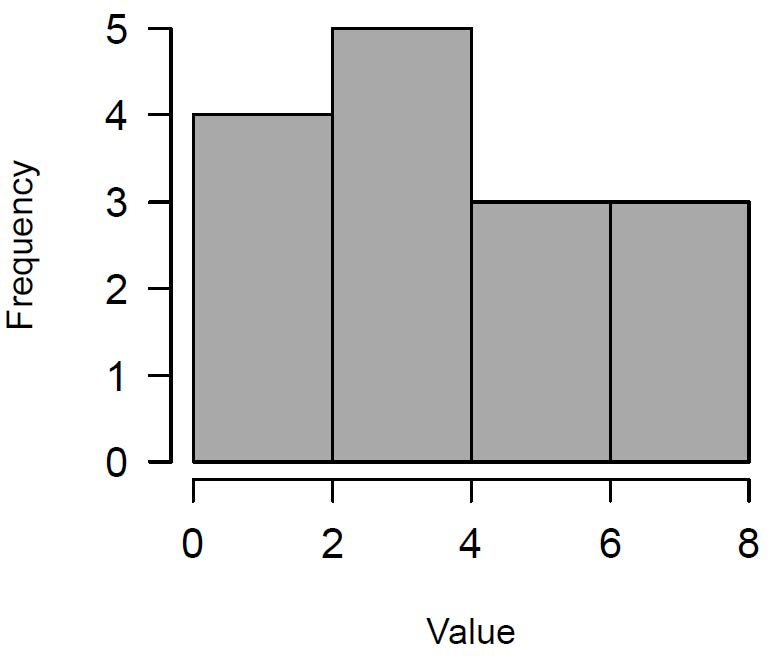
\includegraphics[width=.4\textwidth]{Files/Images/answer2.1b.jpg}
    \end{center}
}

\answerbreakline

\answer{
    2.2 a
}{
    In the plot window you can see that a histogram for the values in the variable \rcode{dataset4} has been drawn by \texttt{R}. \\
    \\
    \answercode{dataset4 <- c(1.5, 5.5, 1.7, 7.2, 1.2, 7.9, 1.4, 3.6, \\
                              3.1, 3.8, 5.9, 3.6, 5.1, 3.2, 7.1) \\
                hist(dataset4)}
}

\answer{
    2.2 b
}{
    The histogram drawn by \texttt{R} has four bars for the ranges 1-2, 3-4, 5-6, and 7-8. The histogram from assignment 2.1b has four bars for the ranges 0-2, 2-4, 4-6, and 6-8. The difference in these two histograms is that they have a different number of bars for different ranges.
}

\answer{
    2.2 c
}{
    \vspace*{-10pt}
    \answercode{{\color{dataset}\# The breaks argument determines the number of bars in the histogram} \\ 
{\color{dataset}\# see ?hist for more help on the hist() function} \\ 
hist(dataset4, breaks = 4)}
}

\answer{
    2.2 d
}{
    \vspace*{-10pt}
    \answercode{hist(dataset4, breaks = 4, col = \textquotesingle blue\textquotesingle,  {\color{dataset}\# col sets the bar color} \\
     xlab = \textquotesingle x-axis\textquotesingle,                     {\color{dataset}\# xlab sets the x-axis name} \\
     ylab = \textquotesingle Frequency\textquotesingle,                  {\color{dataset}\# ylab sets the y-axis name} \\
     main = \textquotesingle My histogram\textquotesingle)               {\color{dataset}\# main sets the title}}
}

\clearpage % Page break

\answer{
    2.2 e
}{
    These data are positively skewed.  \\
    \\
\underline{Explanation}: The mean is higher than the median, and so more values are concentrated on the left side (tail) of the distribution graph while the right tail of the distribution graph is longer. \\
\\
\answercode{mean(dataset4)    {\color{dataset}\# Mean: 4.12} \\
median(dataset4)  {\color{dataset}\# Median: 3.6}}
}

\answerbreakline

\answer{
    2.3 a
}{
    \vspace*{-10pt}
    \answercode{data(swiss)       {\color{dataset}\# Import the swiss data} \\
\\
education   <- swiss\$Education \\
agriculture <- swiss\$Agriculture \\
}
}

\answer{
    2.3 b
}{
    \vspace*{-10pt}
    \answercode{plot(x = education, y = agriculture, \\
     \hspace*{30pt}xlab = \textquotesingle Percentage of education beyond primary school\textquotesingle, \\
     \hspace*{30pt}ylab = \textquotesingle Percentage of males involved in agriculture\textquotesingle)
}
}

\answer{
    2.3 c
}{
    Looking at the scatter plot, there seems to be a tendency for provinces that have a high percentage of education beyond primary school to also have a low percentage of males involved in agriculture.
}

\answer{
    2.3 d
}{
    \vspace*{10pt}
    \answercode{plot(x = education, y = agriculture, \\
     \hspace*{30pt}xlab = \textquotesingle Percentage of education beyond primary school\textquotesingle, \\
     \hspace*{30pt}ylab = \textquotesingle Percentage of males involved in agriculture\textquotesingle, \\
     \hspace*{30pt}col = \textquotesingle blue\textquotesingle, \\ 
     \hspace*{30pt}main = \textquotesingle Provinces in Switzerland\textquotesingle, \\
     \hspace*{30pt}las = 1,           {\color{dataset}\# las sets the rotation of the axis labels} \\
     \hspace*{30pt}bty = \textquotesingle n\textquotesingle)         {\color{dataset}\# bty = \textquotesingle n\textquotesingle removes the outer border lines}
}
}

\answerbreakline

\clearpage % Page break

\answer{
    2.4 a
}{
    \vspace*{-10pt}
    \answercode{data(EuStockMarkets) \\
stockData <- data.frame(EuStockMarkets) \\
\\
plot(stockData\$DAX,  \\
     \hspace*{30pt}type = \textquotesingle l\textquotesingle,         {\color{dataset}\# type = \textquotesingle l\textquotesingle creates lines instead of dots} \\
     \hspace*{30pt}xlab = \textquotesingle Time\textquotesingle, \\
     \hspace*{30pt}ylab = \textquotesingle Price\textquotesingle)
}
}

\answer{
    2.4 b
}{
    \vspace*{-10pt}
    \answercode{{\color{dataset}\# The lines() function adds a line to an existing plot} \\
lines(stockData\$SMI, col = \textquotesingle red\textquotesingle)    {\color{dataset}\# Add a line for the SMI stock} \\
lines(stockData\$CAC, col = \textquotesingle blue\textquotesingle)   {\color{dataset}\# Add a line for the CAC stock} \\
lines(stockData\$FTSE, col = \textquotesingle green\textquotesingle) {\color{dataset}\# Add a line for the FTSE stock}
}
}

\answerbreakline

\answer{
    2.5 a
}{
    \begin{minipage}[t]{.5\textwidth}
    Minimum: 1.2 \\
    Median: 54.2 \\
    Maximum: 89.7 
    \end{minipage}
    \begin{minipage}[t]{.5\textwidth}
    Lower quartile: 35.3 \\
    Upper quartile: 67.8
    \end{minipage} \\
    \\
    \\   
    \answercode{quantile(agriculture, type = 6) \\
{\color{dataset}\# Minimum:        1.2} \\
{\color{dataset}\# Lower quartile: 35.3} \\
{\color{dataset}\# Median:         54.1} \\
{\color{dataset}\# Upper quartile: 67.8} \\
{\color{dataset}\# Maximum:        89.7}
}
}

\answer{
    2.5 b
}{
    \vspace*{-10pt}
    \answercode{boxplot(agriculture)}
}

\answer{
    2.5 c
}{
    The first line creates a vector called \rcode{educationLevel} that contains 47 times \rcode{\textquotesingle 2.Medium\textquotesingle}. The second line changes the \rcode{\textquotesingle 2.Medium\textquotesingle} to \rcode{\textquotesingle 1.Low\textquotesingle} for the provinces that have a percentage of education beyond primary school lower than 6. The third line changes the \rcode{\textquotesingle 2.Medium\textquotesingle} to \rcode{\textquotesingle 3.High\textquotesingle} for the provinces that have a percentage higher than 12. The resulting table shows how many provinces had a percentage lower than 6, between 6 and 12, and higher than 12. \\
    \\
    \answercode{educationLevel <- rep(\textquotesingle2.Medium\textquotesingle, 47)\\
educationLevel[education <= 6] = \textquotesingle1.Low\textquotesingle\\
educationLevel[education >= 12] = \textquotesingle3.High\textquotesingle\\
table(educationLevel)}
}

\clearpage % Page break

\answer{
    2.5 d
}{
    The code creates a box plot of the agriculture variable for each education level \rcode{\textquotesingle 1.Low\textquotesingle}, \rcode{\textquotesingle 2.Medium\textquotesingle}, and \rcode{\textquotesingle 3.High\textquotesingle}.\\
    \\
    \answercode{boxplot(agriculture {\raise.17ex\hbox{$\scriptstyle\sim$}} educationLevel)}
}

\clearpage % Page break                                    
\subsection{Chapter 3: Confidence intervals and hypothesis testing}

\answer{
    3.1 a
}{
    \begin{minipage}[t]{.5\textwidth}
    $N = 4513$ \\
    $n = 100$ \\
    $\bar{x} = 145$ 
    \end{minipage}
    \begin{minipage}[t]{.5\textwidth}
    $s = 25$ \\
    $\sigma = $ unknown \\
    $\mu = $ unknown
    \end{minipage}
}

\answer{
    3.1 b
}{
    $\mu = $ 145 seconds \\
\\
\underline{Explanation}: The best estimate for the population mean $\mu$ is the sample mean $\bar{x}$.
}

\answer{
    3.1 c
}{
    $SE_\mu = \frac{s}{\sqrt{n}} = \frac{25}{\sqrt{100}} = 2.5$
}

\answer{
    3.1 d
}{
    z-value: 2.576 \\
\\
\underline{Explanation}: In table 2 of the formula sheet, the cumulative probability in that lies the closest to 0.995 (split the risk over two sides) is 0.9949. That value can be found at a z-value of 2.576. \\
\\
Lower bound: $\bar{x} - z_{0.995} \times SE_\mu = 145 - 2.567 \times 2.5 = 138.56$ \\
Upper bound: $\bar{x} + z_{0.995} \times SE_\mu = 145 - 2.567 \times 2.5 = 151.44$
}

\answer{
    3.1 e
}{
    $\mu_0 = 150$ (the to be tested limit of 150 seconds for the actual population mean call duration). \\
    \\
    $H_0: \mu \geq \mu_0$ \hspace*{4cm} $H_0: \mu < \mu_0$
}

\answer{
    3.1 f
}{
    Upper bound: $\bar{x} + z_{0.99} \times SE_\mu = 145 - 1.645 \times 2.5 = 149.11$
}

\answer{
    3.1 g
}{
    The upper bound of the confidence interval for $\mu$ is lower than $\mu_0$. $H_0$ is rejected with 99\% confidence. $\mu$ is shown to be significantly lower than 150 seconds. There is a risk of 5\% for a type-I error.
}

\answerbreakline

\clearpage % Page break

\answer{
    3.2 a
}{
    \vspace*{1pt}
    \begin{tabular}{|c|c|r|r|}
    \hline 
    $i$ & $x_i$ & $(x_i - \bar{x})$ & $(x_i - \bar{x})^2$ \tstrut\bstrut\\
    \hline
    1 & 3.03 & -0.0863 & 0.0074 \tstrut\bstrut\\
    \hline
    2 & 3.45 & 0.3338 & 0.1114 \tstrut\bstrut\\
    \hline
    3 & 3.94 & 0.8238 & 0.6786 \tstrut\bstrut\\
    \hline
    4 & 2.34 & -0.7763 & 0.6026 \tstrut\bstrut\\
    \hline
    5 & 3.34 & 0.2238 & 0.0501 \tstrut\bstrut\\
    \hline
    6 & 2.53 & -0.5863 & 0.3437 \tstrut\bstrut\\
    \hline
    7 & 2.88 & -0.2363 & 0.0558 \tstrut\bstrut\\
    \hline
    8 & 3.42 & 0.3038 & 0.0923 \tstrut\bstrut\\
    \hline
    \end{tabular} \\
    \\
    $\sum x_i = 24.93$  \hspace*{.4cm} $\sum (x_i - \bar{x})^2 = 1.9418$ \\
    \\
    \hspace*{10pt} $\bar{x} = 3.116$ \hspace*{2cm} $s^2 = 0.277$ \\
}

\answer{
    3.2 b
}{
    Hartley's F: $\frac{s^2_min}{s^{max}} = \frac{1.113}{0.227} = 4.018$
}

\answer{
    3.2 c
}{
    $H_0: \sigma^2_1 = \sigma^2_2 = \sigma^2_3$ \hspace*{4cm} $H_0: \sigma^2_1 \neq \sigma^2_2 \neq \sigma^2_3$
}

\answer{
    3.2 d
}{
    Hartley's $F_{max}$: 6.94
}

\answer{
    3.2 e
}{
    The value $F = 4.018$ is lower than critical value $F_{max} = 6.94$. $H_0$ is not rejected. There is no indication the variance for these months is not homogeneous. There is a risk of a type-II error.
}

\answerbreakline

\answer{
    3.3 a
}{
    \vspace*{-10pt}
    \answercode{{\color{dataset}\# Be sure to set your working directory when providing a relative path} \\
dataset5 <- read.csv(\textquotesingle populations.csv\textquotesingle)}
}

\answer{
    3.3 b
}{
    The code creates four random samples of size 90 from the columns \rcode{P1} - \rcode{P4} in the data frame called \rcode{dataset5}. The seed makes sure that you can recreate the same random samples again, so that if you close \texttt{R} and continue tomorrow we get the same samples. \\
    \\
    \answercode{set.seed(54321) {\color{dataset} \# You can replace 54321 with your own seed number} \\
\\
sample1 <- sample(dataset5\$P1, size = 90)\\
sample2 <- sample(dataset5\$P2, size = 90)\\
sample3 <- sample(dataset5\$P3, size = 90)\\
sample4 <- sample(dataset5\$P4, size = 90)}
}

\clearpage % Page break

\answer{
    3.3 c
}{
    Standard error sample 1: 29.24 \\
    Standard error sample 2: 7.64 \\
    Standard error sample 3: 30.61 \\
    Standard error sample 4: 18.09 \\
    \\
    \answercode{{\color{dataset}\# Means} \\
x1 <- mean(sample1) {\color{dataset} \# Mean: 456.78} \\
x2 <- mean(sample2) {\color{dataset} \# Mean: 511.02} \\
x3 <- mean(sample3) {\color{dataset} \# Mean: 790.32} \\
x4 <- mean(sample4) {\color{dataset} \# Mean: 533.37} \\
\\
{\color{dataset} \# Standard deviations} \\
sd1 <- sd(sample1) {\color{dataset} \# Standard deviation: 277.38} \\
sd2 <- sd(sample2) {\color{dataset} \# Standard deviation: 72.43} \\
sd3 <- sd(sample3) {\color{dataset} \# Standard deviation: 290.46} \\
sd4 <- sd(sample4) {\color{dataset} \# Standard deviation: 171.58} \\
\\
{\color{dataset} \# Standard errors se = sd / sqrt(n)} \\
se1 <- sd1 / sqrt(length(sample1))    {\color{dataset} \# Standard error: 29.24} \\
se2 <- sd2 / sqrt(length(sample2))    {\color{dataset} \# Standard error: 7.64} \\
se3 <- sd3 / sqrt(length(sample3))    {\color{dataset} \# Standard error: 30.61} \\
se4 <- sd4 / sqrt(length(sample4))    {\color{dataset} \# Standard error: 18.09}
    }
}

\answer{
    3.3 d
}{
    The value 1.644854 comes from the standard normal distribution with $\mu = 0$ and $\sigma = 1$. This is the z-value for a 95\% one-sided confidence interval (or a 90\% two-sided confidence interval).
}

\answer{
    3.3 d
}{
    \vspace*{-10pt}
    \answercode{{\color{dataset} \# Gives the left-tailed probability (z-value) for 95\% confidence} \\
qnorm(p = 0.95) {\color{dataset} \# 1.645}}
}

\answer{
    3.3 e
}{
    In a 95\% confidence interval there is 2.5\% of the risk at the lower bound and 2.5\% of the risk at the upper bound. You can therefore use the 97.5\% quantile of the standard normal distribution to get the z-value for a two-sided 95\% confidence interval and use it for both upper and lower bound. \\
    \\
    \answercode{z <- qnorm(p = 0.975)}
}

\clearpage % Page break

\answer{
    3.3 f
}{
    \vspace*{-10pt}
    \answercode{{\color{dataset} \# Lower bounds} \\
lb1 <- x1 - z * se1 {\color{dataset}\# Lower bound: 399.48} \\
lb2 <- x2 - z * se2 {\color{dataset}\# Lower bound: 496.06} \\
lb3 <- x3 - z * se3 {\color{dataset}\# Lower bound: 730.31} \\
lb4 <- x4 - z * se4 {\color{dataset}\# Lower bound: 497.92} \\
 \\
{\color{dataset}\# Upper bounds} \\
ub1 <- x1 + z * se1 {\color{dataset}\# Upper bound: 514.10} \\
ub2 <- x2 + z * se2 {\color{dataset}\# Upper bound: 525.99} \\
ub3 <- x3 + z * se3 {\color{dataset}\# Upper bound: 850.33} \\
ub4 <- x4 + z * se4 {\color{dataset}\# Upper bound: 568.81}}
}

\answer{
    3.3 g
}{
    \vspace*{1pt}
    \begin{center}
    \begin{tabular}{r|c|c|c|c|}
    \multicolumn{1}{c}{} & \multicolumn{1}{c}{\rcode{sample1}} & \multicolumn{1}{c}{\rcode{sample2}} & \multicolumn{1}{c}{\rcode{sample3}} & \multicolumn{1}{c}{\rcode{sample4}} \tstrut\bstrut\\
    \cline{2-5}
    \rcode{ub} & 514.10 & 525.99 & 850.33 & 568.81 \tstrut\bstrut\\
    \cline{2-5}
    \rcode{x} & 456.78 & 511.01 & 790.32 & 533.37 \tstrut\bstrut\\
    \cline{2-5}
    \rcode{lb} & 399.48 & 496.06 & 730.31 & 497.92 \tstrut\bstrut\\
    \cline{2-5}
    \end{tabular}
    \end{center}
    
    \begin{center}
    \begin{tabular}{r|c|c|c|c|}
    \multicolumn{1}{c}{} & \multicolumn{1}{c}{\rcode{P1}} & \multicolumn{1}{c}{\rcode{P2}} & \multicolumn{1}{c}{\rcode{P3}} & \multicolumn{1}{c}{\rcode{P4}} \tstrut\bstrut\\
    \cline{2-5}
    \rcode{mu} & 495.54 & 500.08 & 748.96 & 556.43 \tstrut\bstrut\\
    \cline{2-5}
    \textit{mu in interval?} & YES & YES & YES & YES \tstrut\bstrut\\
    \cline{2-5}
    \end{tabular}
    \end{center}
    \\
    \answercode{{\color{dataset}\# Population means} \\
mu1 <- mean(dataset5\$P1) {\color{dataset}\# Mean: 495.54} \\
mu2 <- mean(dataset5\$P2) {\color{dataset}\# Mean: 500.08} \\
mu3 <- mean(dataset5\$P3) {\color{dataset}\# Mean: 748.96} \\
mu4 <- mean(dataset5\$P4) {\color{dataset}\# Mean: 556.43}}
}

\answer{
    3.3 h
}{
    Yes, in this case all population means are inside the intervals.
}

\answer{
    3.3 i
}{
    The population mean will fall inside the interval 95 out of a 100 times (95\% confidence). This means that about 1 in 20 confidence intervals will not have the true population mean between their lower and upper bound.
}

\answerbreakline

\clearpage % Page break

\answer{
    3.4 a
}{
    \vspace*{-10pt}
    \answercode{{\color{dataset}\# install.packages(\textquotesingle car\textquotesingle)} \\
library(car)  \\
 \\
{\color{dataset}\# This create a 2x2 layout} \\
layout(matrix(c(1, 2, 3, 4), byrow = TRUE, nrow = 2)) \\
 \\
hist(sample1, col = \textquotesingle gray\textquotesingle) \\
hist(sample2, col = \textquotesingle gray\textquotesingle) \\
hist(sample3, col = \textquotesingle gray\textquotesingle) \\
hist(sample4, col = \textquotesingle gray\textquotesingle) \\
 \\
{\color{dataset}\# This resets the layout to the default (1 plot)} \\
layout(1)
}
}

\answer{
    3.4 b
}{
    Sample 2 looks like it might come from a normal distribution.
}

\answer{
    3.4 c
}{
    \vspace*{-10pt}
    \answercode{{\color{dataset}\# This create a 2x2 layout} \\
layout(matrix(c(1, 2, 3, 4), byrow = TRUE, nrow = 2)) \\
 \\
qqPlot(sample1, distribution = \textquotesingle norm\textquotesingle) \\
qqPlot(sample2, distribution = \textquotesingle norm\textquotesingle) \\
qqPlot(sample3, distribution = \textquotesingle norm\textquotesingle) \\
qqPlot(sample4, distribution = \textquotesingle norm\textquotesingle) \\
 \\
{\color{dataset}\# This resets the layout to the default (1 plot)} \\
layout(1)
}
}

\clearpage % Page break

\answer{
    3.5 d
}{
    The \rcode{sample1} histogram looks normal in the middle, but has too many low and too many high values. This can be seen in the qqplot by the dots on the left of the diagonal at the bottom and the dots on the right at the top. \\
\\
The \rcode{sample2} histogram looks normal so the dots in the qqplot are almost everywhere on the diagonal. Only in the right part of the middle the histogram frequency is a bit too low, this is reflected in the dots below the diagonal around zero in the qqplot.\\

The \rcode{sample3} histogram is too high on the sides (or too low in the middle) to be normal. This can be seen in the qqplot by the dots on the left of the diagonal at the bottom and the dots on the right at the top.\\
\\
\rcode{sample4} is negatively skewed. This can be seen in the qqplot from the arch shape; the left of the histogram is too low causing the dots on the right of the diagonal and the right of the histogram is too high also causing dots to the right of the diagonal.
}

\answer{
    3.4 e
}{
    $H_0$: The sample is normally distributed\\
    $H_1$: The sample is not normally distributed
}

\answer{
    3.4 f
}{
    Samples 1, 3, and 4 are not normally distributed, since the p-value is lower than 1\% (for 99\% confidence). Sample 2 is normally distributed, since the p-value is higher than 1\%. \\
    \\
    \answercode{shapiro.test(sample1) {\color{dataset}\# p-value: 0.0022} \\
shapiro.test(sample2) {\color{dataset}\# p-value: 0.949} \\
shapiro.test(sample3) {\color{dataset}\# p-value: 0.0068} \\
shapiro.test(sample4) {\color{dataset}\# p-value: 0.0001}}
}

\answer{
    3.4 g
}{
    When the sample is not normally distributed, the sample can be used to estimate the population mean. \\
 \\
\underline{Explanation}: This method to estimate the population mean assumes the distribution of sample means to be normally distributed. It does not assume a normally distributed sample. The Central Limit Theorem states that any sample large enough ($n \geq 30$) will have a normal distribution of sample means, so you can use this method here ($n = 90$) without problems.
}

\answerbreakline

\clearpage

\answer{
    3.5 a
}{  
    \vspace*{-10pt}
    \answercode{library(car) \\
data(iris) \\
 \\
plot(x = iris\$Species, y = iris\$Sepal.Length, \\
     \hspace*{20pt}col = \textquotesingle grey\textquotesingle, main = \textquotesingle Sepal Length\textquotesingle) \\
 \\
plot(x = iris\$Species, y = iris\$Sepal.Width, \\
     \hspace*{20pt}col = \textquotesingle grey\textquotesingle, main = \textquotesingle Sepal Width\textquotesingle)
}
}

\answer{
    3.5 b
}{
    Looking at the width of the range and quartile ranges: For sepal length the variance for setosa looks much smaller than for the other two species, for sepal width all variances look similar.
}

\answer{
    3.5 c
}{
    $H_0: \sigma^2_1 = \sigma^2_2 = \sigma^2_3$ \hspace*{4cm} $H_0: \sigma^2_1 \neq \sigma^2_2 \neq \sigma^2_3$
}

\answer{
    3.5 d
}{
    The p-value for the sepal length is lower than 10\%. This implies that $H_0$ is rejected. This means that the variance of the sepal length over the species is not homogeneous. There is a 5\% change of a type-I error. \\
\\
The p-value for the sepal with is not lower than 10\%. This implies that $H_0$ is not rejected. This means that there is no indication that the variance of the sepal width over the species is not homogeneous. There is a risk of a type-II error. \\
\\
\answercode{{\color{dataset}\# Levene's Test for Homogeneity of Variance} \\
leveneTest(y = iris\$Sepal.Length,  \\
           group = iris\$Species) {\color{dataset}\# p-value: 0.002259} \\
 \\
leveneTest(y = iris\$Sepal.Width,  \\
           group = iris\$Species) {\color{dataset}\# p-value: 0.5555}}
}

\clearpage % Page break                                
\subsection{Chapter 4: Correlation and regression}

\answer{
    4.1 a
}{
    Two variables can either be positively related, not related, or negatively related. The most logical relationship is that the distance a customer lives from the store is negatively related to how many times they visit the store.
}

\answer{
    4.1 b
}{
    \vpsace*{1pt}
    \begin{tabular}{|c|c|r|r|r|r|}
    \hline 
    $i$ & $x_i$ & $y_i$ & $(x_i - \bar{x})$ & $(y_i - \bar{y})$ & $(x_i - \bar{x})(y_i - \bar{y})$ \tstrut\bstrut\\
    \hline
    1 & 4.87 & 2.90 & 1.868 & -1.09 & -2.053 \tstrut\bstrut\\
    \hline
    2 & 3.04 & 4.50 & 0.038 & 0.501 & 0.0194 \tstrut\bstrut\\
    \hline
    3 & 1.65 & 4.94 & -1.351 & 0.941 & -1.272 \tstrut\bstrut\\
    \hline
    4 & 2.88 & 3.28 & -0.121 & -0.718 & 0.087 \tstrut\bstrut\\
    \hline
    5 & 2.31 & 4.73 & 0.691 & 0.731 & -0.505 \tstrut\bstrut\\
    \hline
    6 & 3.96 & 2.64 & 0.958 & -1.358 & -1.303 \tstrut\bstrut\\
    \hline
    7 & 2.70 & 3.70 & -0.301 & -0.298 & 0.089 \tstrut\bstrut\\
    \hline
    8 & 2.60 & 5.30 & -0.401 & 1.301 & -0.522 \tstrut\bstrut\\
    \hline
    \end{tabular}\\
    \\
    \hspace*{.5cm} $\bar{x} = 3.001$ \hspace*{1cm} $\sum (x_i - \bar{x})(y_i - \bar{y}) = -5.458$ \\
    \\
    \hspace*{.5cm} $\bar{y} = 3.998$ \hspace*{3.1cm} $n - 1 = 7$ \\
    \\
    \hspace*{6cm} $s_{xy} = -0.779$ \\
}

\answer{
    4.1 c
}{
    The covariance is negative. A negative covariance indicates that that as one variable deviates from the mean, the other variable deviates in the other direction. This means that, when a customer’s distance from the store in kilometers is higher than the mean, their average visits per week will likely be lower than the mean.
}

\answer{
    4.1 d
}{
    The disadvantage of using the covariance as a measure for the strength of this relationship is that it depends on the measurement unit (kilometers vs. meters) that the co-worker asks the questions in. If the co-worker would have asked the question in meters the covariance would have increased by a 1000 times, namely -779.84.
}

\answer{
    4.1 e
}{
    $s_x = \sqrt{\frac{\sum^n_{i = 1} (x_i - \bar{x})^2}{n - 1}} = \sqrt{\frac{6.977}{7}} = 0.998$ \hspace*{2cm} $s_y = \sqrt{\frac{\sum^n_{i = 1} (y_i - \bar{y})^2}{n - 1}} = \sqrt{\frac{7}{7}} = 1$
}

\answer{
    4.1 f
}{
    $r_{xy} = \frac{s_{xy}}{s_x \times s_y} = \frac{-0.779}{0.998 \times 1} = -0.779$
}

\answer{
    4.1 g
}{
    The coefficient is -0.779, which represents is a relatively strong negative relationship.
}

\answerbreakline 

\clearpage

\answer{
    4.2 a
}{
    $H_0$: $\rho_{xy} \geq 0$ \hspace{4cm} $H_1$: $\rho_{xy} < 0$
}

\answer{
    4.2 b
}{
    \begin{minipage}[t]{.5\textwidth}
    $N = $ unknown \\
    $n = 8$ 
    \end{minipage}
    \begin{minipage}[t]{.5\textwidth}
    $r_{xy} = -0.779$ \\
    $\rho_{xy} = $ unknown
    \end{minipage}
}

\answer{
    4.2 c
}{
    $z_{0.05} = -1.645$
}

\answer{
    4.2 d
}{
    $z_r = \frac{1}{2} \times log_e(\frac{1 + r}{1 - r}) = \frac{1}{2} \times log_e(\frac{1 - 0.779}{1 + 0.779}) = -1.043$ \\
    \\
    $SE_r = \frac{1}{\sqrt{n - 3}} = \frac{1}{\sqrt{8 - 3}} = 0.447$ \\
    \\
    $z_{xy} = \frac{z_r}{SE_r} = \frac{-1.043}{0.447} = -2.33$
}

\answer{
    4.2 e
}{
    The observed z-value is more extreme (lower) than the critical z-value. $H_0$ is rejected with 95\% confidence. You can be 95\% confident that $\rho_{xy}$ is negative in the population. There is a 5\% change of a type-I error.
}

\answerbreakline

\answer{
    4.3 a
}{
    \vspace*{-10pt}
    \answercode{{\color{dataset}\# Be sure to set your working directory when providing a relative path} \\
dataset6 <- read.csv(\textquotesingle localSupermarket.csv\textquotesingle)}
}

\answer{
    4.3 b
}{
    Covariance: -0.30 \\
    Correlation: -0.30 \\
    \\
     \answercode{cov(dataset6\$Distance, dataset6\$AvgVisits)  {\color{dataset}\# Covariance   -0.3000603} \\
cor(dataset6\$Distance, dataset6\$AvgVisits)  {\color{dataset}\# Correlation: -0.3000382}}   
}

\answer{
    4.3 c
}{
    \vspace*{-10pt}
    \answercode{cor.test(dataset6\$Distance, dataset6\$AvgVisits, alternative = \textquotesingle less\textquotesingle) \\
{\color{dataset}\# Correlation: -0.30} \\
{\color{dataset}\# t-value: -9.936} \\
{\color{dataset}\# p-value: < 2.2e-16}}
}

\answer{
    4.3 d
}{
    The black line represents the normal distribution. The red line represents the t-distribution. The difference between the two distributions, in terms of their shape, is that the t-distribution has slightly thicker tails. When you increase the degrees of freedom of the t-distribution, it will start to look more like the normal distribution.\\
    \\
    \answercode{curve(dnorm(x, mean = 0, sd = 1), from = -3, to = 3, ylab = \textquotesingle Density\textquotesingle)\\
curve(dt(x, df = 3), from = -3, to = 3, add = TRUE, col = \textquotesingle red\textquotesingle)}
}

\clearpage

\answer{
    4.3 e
}{
    $df = 998$ \hspace*{5cm} $t_{xy} = -9.936$ \\
    \\
    \answercode{n <- nrow(dataset6) \\
dft <- n - 2 {\color{dataset}\# 998} \\
 \\
r <- cor(dataset6\$Distance, dataset6\$AvgVisits) \\
tscore <- r * sqrt(n - 2) / sqrt(1 - r\textrm{\textasciicircum}2)    \\
{\color{dataset}\# t-score: -9.936 so you can confirm the value in 4.3c}
}
}

\answer{
    4.3 f
}{
    You can find the t-value in the bottom line of the output in the console.
}

\answer{
    4.3 g
}{
    The p-value is < 2.2e-16, which is lower than the significance level of 5\%. This means that $H_0$ can be rejected with 95\% confidence.
}

\answerbreakline

\answer{
    4.4 a
}{
    \vspace*{-10pt}
    \answercode{{\color{dataset}\# Be sure to set your working directory when providing a relative path} \\
dataset7 <- read.csv(\textquotesingle nationalSupermarket.csv\textquotesingle)}
}

\answer{
    4.4 b
}{
    \vspace*{-10pt}
    \answercode{plot(x = dataset7\$Price, \\
     \hspace*{30pt}y = dataset7\$AvgWasted, \\
     \hspace*{30pt}main = \textquotesingle Scatter plot of Price vs. AvgWasted\textquotesingle, \\
     \hspace*{30pt}ylab = \textquotesingle Average number of cartons wasted\textquotesingle, \\
     \hspace*{30pt}xlab = \textquotesingle Price of a carton of milk\textquotesingle, \\
     \hspace*{30pt}las = 1, \\
     \hspace*{30pt}col = \textquotesingle orange\textquotesingle, \\
     \hspace*{30pt}pch = 19, \\
     \hspace*{30pt}bty = \textquotesingle n\textquotesingle)
}
}

\answer{
    4.4 c
}{
    AvgWasted $= \beta_0 + \beta_1 \,\times$ Price
}

\answer{
    4.4 d
}{
    \vspace*{-10pt}
    \answercode{lmfit <- lm(formula = AvgWasted {\raise.17ex\hbox{$\scriptstyle\sim$}} Price, data = dataset7)}
}

\answer{
    4.4 e
}{
    AvgWasted $= 0.236 + 2.995 \,\times$ Price \\
    \\
    \answercode{summary(lmfit) \\
{\color{dataset}\# b0 = 0.236} \\
{\color{dataset}\# b1 = 2.995} \\
{\color{dataset}\# R-squared: 0.64}
}
}

\clearpage % Page break

\answer{
    4.4 f
}{
    \vspace*{-10pt}
    \answercode{abline(lmfit)}
}

\answer{
    4.4 g
}{
    $R^2 = 0.64$ \\
    \\
    Interpretation: The multiple $R^2$ is 0.64, meaning that 64\% of the variation in the number of milk cartons that are thrown away each day can be explained by the price of the milk cartons.
}

\answer{
    4.4 h
}{
    $H_0$: $\beta_1 \leq 0$ \hspace*{4cm} $H_1$: $\beta_1 > 0$
}

\answer{
    4.4 i
}{
    The p-value for the regression coefficient is < 2e-16, which is lower than the significance level of 5\%. $H_0$ can be rejected with 95\% confidence. You can be 95\% sure that $\beta_1$ is positive in the population. The price contributes significantly to the average number of milk cartons thrown away. There is a 5\% risk of a type-I error.
}

\answerbreakline

\answer{
    4.5 a
}{
    \vspace*{-10pt}  
    \answercode{newdata <- data.frame(Price = 0.70)}
}

\answer{
    4.5 b
}{
    Predicted value: 2.33 \\
    \\
    \answercode{predict(object = lmfit, \\
        \hspace*{40pt}newdata = newdata) {\color{dataset}\# Prediction: 2.33}}
}

\answer{
    4.5 c
}{
    Predicted value: $0.236 + 2.995 \times 0.70 = 2.33$
}

\answer{
    4.5 d
}{
    \vspace*{-10pt}
    \answercode{predict(object = lmfit, newdata = newdata, \\
        \hspace*{40pt}interval = \textquotesingle prediction\textquotesingle, level = 0.90) \\
{\color{dataset}\# Lower bound: 0.734} \\
{\color{dataset}\# Upper bound: 3.931}
}
}

\answer{
    4.5 e
}{
    The supermarket will throw away fewer cartons of milk. \\
    \\
    \underline{Explanation}: The current number of milk cartons thrown away (4) lies outside the bounds of the 90\% confidence interval for the prediction.
}

\clearpage % Page break                                    
\subsection{Chapter 5: Comparing one or two means}

\answer{
    5.1 a
}{
    $n = 49$ \\
    $\bar{x} = 0.918$ \\
    $s = 0.071$ \\
    $\mu_0 = 0.9$
}

\answer{
    5.1 b
}{
    $H_0$: $\mu_0 \leq 0.9$ \hspace{4cm} $H_1$: $\mu_0 > 0.9$
}

\answer{
    5.1 c
}{
    Lower bound: $\bar{x} - z_{\alpha} \times SE_\mu = 0.918 - 1.645 \times \frac{0.071}{\sqrt{49}} = 0.901$
}

\answer{
    5.1 d
}{
    The lower bound of the confidence interval for $\mu$ is higher than $\mu_0$. $H_0$ is rejected with 95\% confidence. The PFAS level in town is significantly higher than 0.9 microgram/kg dry soil. There is a risk of 5\% for a type-I error.
}

\answer{
    5.1 e
}{
    z-score: $\frac{\bar{x} - \mu}{\nicefrac{s}{\sqrt{n}}} = \frac{0.918 - 0.9}{\nicefrac{0.071}{\sqrt{49}}} = 1.775$
}

\answer{
    5.1 f
}{
    The critical z-value for 95\% confidence is 1.645. The p-value (the probability that $H_0$ is true) is 0.05. For any z-value higher than 1.645 the p-value is lower than 0.05. Since for this test the (absolute of the) calculated z-score  = 1.775 and this is higher than 1.645, this means that the p-value is lower than 0.05. \\
\\
Note:  For right sided tests the z-score is negative, but since the standard normal distribution is symmetric we can simply use the positive value for comparing it with the critical z-value.
}

\answer{
    5.1 g
}{
    The calculated z-score is more extreme (higher) than the critical z-value of 1.645. $H_0$ is rejected with 95\% confidence. The PFAS level in town is significantly higher than 0.9 microgram/kg dry soil. There is a risk of 5\% for a type-I error. The two methods produce the same answer. It cannot be different; the methods are equivalent.
}

\answer{
    5.1 h
}{
    t-score: $\frac{\bar{x} - \mu}{\nicefrac{s}{\sqrt{n}}} = \frac{0.930 - 0.9}{\nicefrac{0.070}{\sqrt{16}}} = 1.714$
}

\answer{
    5.1 i
}{
  The calculated t-score of 1.714 is lower than the critical t-value of 1.753. $H_0$ is not rejected. The PFAS level in town is significantly below the norm. There is a risk type-II error.  
}

\answer{
    5.1 j
}{
    Lower bound: $\bar{x} - t_{\alpha (df = 15)} \times SE_\mu = 0.930 - 1.753 \times \frac{0.070}{\sqrt{16}} = 0.899$
}

\answer{
    5.1 k
}{
    Yes. The lower bound for the population mean $\mu$ is 0.899, it can therefore not be ruled out that the mean PFAS level is below 0.9.
}

\answer{
    5.1 l
}{
    The sample is so much smaller (16 vs. 49) that there is too much uncertainty in the result.
}

\answerbreakline

\clearpage % Page break

\answer{
    5.2 a
}{
    Result: 1.645 \\
    \\
    This is the z-value for a 95\% one-sided confidence interval. \\
    \\
    \answercode{qnorm(p = 0.95, mean = 0, sd = 1, lower.tail = TRUE) \\
{\color{dataset}\# Or because the standard normal distribution is the default simply use:}  \\
qnorm(0.95) {\color{dataset}\# 1.645}}
}

\answer{
    5.2 b
}{
    Because for a two-sided interval you spread the risk over the two tails. There is 2.5\% of risk on the left tail and 2.5\% of risk on the right tail. \\
    \\
    \answercode{qnorm(p = 0.975) {\color{dataset}\# 1.960}}
}

\answer{
    5.2 c
}{
    The \rcode{pnorm()} is the inverse of the \rcode{qnorm()} function: It returns the cumulative probability for a given value \rcode{q} in a specified normal distribution. \\
    \\
    \answercode{pnorm(q = 1.645, mean = 0, sd = 1) {\color{dataset}\# 0.95} \\
pnorm(1.960) {\color{dataset}\# 0.975}}
}

\answer{
    5.2 d
}{
    The \rcode{qt()} function returns the t-value for a given cumulative probability \rcode{p} and given number of degrees of freedom \rcode{df}. \\
    \\
    \answercode{qt(p = 0.95, df = 15) {\color{dataset}\# 1.753}}
}

\answer{
    5.2 e
}{
    The \rcode{pt()} is the inverse of the \rcode{qt()} function: It returns the cumulative probability for a given value \rcode{q} in a specified t-distribution. \\
    \\
    \answercode{pt(q = 1.753, df = 15) {\color{dataset}\# 0.95}}
}

\answer{
    5.2 f
}{
\vspace*{1pt}
    \begin{minipage}{.5\textwidth}
    t$_1$: -1.06 \\
    t$_3$: 1.328
    \end{minipage}
        \begin{minipage}{.5\textwidth}
            t$_2$: -1.328 \\
    t$_4$: 1.328
    \end{minipage} \\
    \\
    \\
    \answercode{qt(p = 0.15, df = 19)                       {\color{dataset}\# -1.06} \\
qt(p = 0.10, df = 19)                       {\color{dataset}\# -1.328} \\
qt(p = 0.90, df = 19)                       {\color{dataset}\# 1.328} \\
qt(p = 0.10, df = 19, lower.tail = FALSE)   {\color{dataset}\# 1.328}}
}

\clearpage % Page break

\answer{
    5.2 g
}{
    \begin{minipage}{.3\textwidth}
    p$_1$: 0.081 
    \end{minipage}
        \begin{minipage}{.3\textwidth}
            p$_2$: 0.929 
    \end{minipage}
            \begin{minipage}{.3\textwidth}
            p$_2$: 0.015
    \end{minipage} \\
    \\
    \answercode{pt(q = -1.5, df = 11)                     {\color{dataset}\# 0.081} \\
diff(pt(q = c(-2,2), df = 11))            {\color{dataset}\# 0.929} \\
pt(q = 2.5, df = 11, lower.tail = FALSE)  {\color{dataset}\# 0.015}}
}

\answer{
    5.2 h
}{
    Two tailed inequality test: 2.467 \\
One-tailed right sided test: 2.153 \\
One-tailed left sided test: -2.153 \\
\\
\answercode{{\color{dataset}\# Two-tailed inequality test} \\
qt(p = 0.99, df = 28)  {\color{dataset}\# 2.467}   \\
 \\
{\color{dataset}\# One-tailed right sided test}      \\             
qt(p = 0.98, df = 28)  {\color{dataset}\# 2.153} \\
 \\
{\color{dataset}\# One-tailed left sided test} \\
qt(p = 0.98, df = 28, lower.tail = FALSE) {\color{dataset}\# -2.153}}
}

\answer{
    5.2 i
}{
    Two-tailed inequality test: $H_0$ rejected (2.6 > 2.476) \\
One-tailed right sided test: $H_0$ rejected (-2.3 < -2.153) \\
One-tailed left sided test: $H_0$ not rejected (1.6 < 2.153) \\

}

\answerbreakline

\answer{
    5.3 a
}{
    Because different men get the caffeine and the placebo. There are 18 unique test subjects. Everyone gets tested once and every measurement is therefore independent.
}

\answer{
    5.3 b
}{
    $H_0$: $\mu_1 \leq \mu_2$ \hspace{4cm} $H_1$: $\mu_1 > \mu_2$
}

\answer{
    5.3 c
}{
    $\s^2_p = \frac{(n_1 - 1) s_1^2 + (n_2 - 1) s_2^2}{n_1 + n_2 - 2)} = \frac{(9 - 1) \times 5.61^2 + (9 - 1) \times 7.70^2}{9 + 9 - 2} = 45.38$
}

\answer{
    5.3 d
}{
    $t = \frac{(x_1 - x_2) - D_0}{\sqrt{s^2_p (\frac{1}{n_1} + \frac{1}{n_2})}} = \frac{(94.22 - 100.56)}{\sqrt{45.38 \times (\frac{1}{9} + \frac{1}{9})}} = 1.995$
}

\answer{
    5.3 e
}{
    The calculated t-score of 1.995 is more extreme (higher) than the critical value of 1.746. $H_0$ is rejected with 95\% confidence. The mean placebo RER level is significantly higher than the mean caffeine RER level. There is a risk of 5\% for type-I error.

}

\clearpage % Page break

\answer{
    5.3 f
}{
    \vspace*{-7.5pt}
    \begin{minipage}[t]{0.5\textwidth}
    \rcode{placebo}	\\
Mean: 	100.55 \\
Standard deviation: 7.699
    \end{minipage}
    \begin{minipage}[t]{0.5\textwidth}
    \rcode{caffeine} \\
    Mean: 94.22 \\
    Standard deviation: 5.607
    \end{minipage} \\
    \\
    \\
    \answercode{{\color{dataset}\# These are the values for the RER test data set} \\
placebo <- c(105, 119, 100, 97, 96, 101, 94, 95, 98) \\
caffeine <- c(96, 99, 94, 89, 96, 93, 88, 105, 88) \\
 \\
 \\
mean(placebo)  {\color{dataset}\# Mean:                 100.55} \\
sd(placebo)    {\color{dataset}\# Standard deviation:   7.699}   \\
 \\
mean(caffeine) {\color{dataset}\# Mean:                 94.22}\\
sd(caffeine)   {\color{dataset}\# Standard deviation:   5.607} }
}

\answer{
    5.3 g
}{
    The code runs an independent (not paired) samples t-test with a confidence of 95\% for \rcode{placebo} and \rcode{caffeine}, with the alternative hypothesis $H_1$ that the difference in means is greater than 0. The variances are assumed equal. \\
    \\
    \answercode{t.test(x = placebo, y = caffeine, alternative = \textquotesingle greater\textquotesingle, mu = 0, \\
\hspace*{40pt}paired = FALSE, var.equal = TRUE, conf.level = 0.95)
}
}

\answer{
    5.3 h
}{
    The Welch Two Sample t-test leads to a slightly different p-value of 0.03252, but the same conclusion: rejection of $H_0$. \\
    \\
    \answercode{t.test(x = placebo, y = caffeine, alternative = \textquotesingle greater\textquotesingle, mu = 0, \\
\hspace*{40pt}paired = FALSE, var.equal = FALSE, conf.level = 0.95)
}
}

\answer{
    5.3 i
}{
    You can use Hartley’s F or Levene’s test.
}

\answerbreakline

\answer{
    5.4 a
}{
    The observations are not independent because the same twelve people are tested twice. The two blood pressure measurements for one person are connected/dependent: a person with high blood pressure will have higher values in both experiments. That is why in a dependent t-test you look at the difference between the two measurements.
}

\clearpage % Page break

\answer{
    5.4 b
}{
    Mean standing: 140.83 \\
Mean lying: 143.33 \\
Mean difference: 2.5 \\
\\
\answercode{{\color{dataset}\# These are the values for the blood pressure data set} \\
standing <- c(132, 146, 135, 141, 139, 162, 128, 137, 145, 151, 131, 143) \\
lying <- c(136, 145, 140, 147, 142, 160, 137, 136, 149, 158, 120, 150) \\
 \\
mean(standing)   {\color{dataset}\# Mean standing: 140.83} \\
mean(lying)      {\color{dataset}\# Mean lying: 143.33} \\
differences <- lying - standing \\
mean(differences) {\color{dataset}\# Mean difference: 2.5}}
}

\answer{
    5.4 c
}{
    $H_0$: $\mu_D \leq 0$ \hspace*{4cm} $H_1$: $\mu_D > 0$
}

\answer{
    5.4 d
}{
    The test is done with \rcode{alternative = \textquotesingle greater\textquotesingle}, which means that now \texttt{R} will test for standing greater than lying, which is quite improbable given the sample results. \\
    \\
    \answercode{t.test(x = standing, y = lying, alternative = \textquotesingle greater\textquotesingle, mu = 0, \\
\hspace*{40pt}paired = TRUE, conf.level = 0.925)}
}

\answer{
    5.4 e
}{
    The p-value for this sample outcome is 0.07189, which is below the limit of 0.075 (92.5\% confidence). $H_0$ is rejected with 92.5\% confidence. The blood pressure is significantly higher lying down than standing up. There is a risk of 7.5\% for type-I error. \\
    \\
    \answercode{{\color{dataset}\# Correct: alternative = \textquotesingle less\textquotesingle} \\
    t.test(x = standing, y = lying, alternative = \textquotesingle less\textquotesingle, mu = 0, \\
\hspace*{40pt}paired = TRUE, conf.level = 0.925)}
}

\clearpage % Page break                                     
\subsection{Chapter 6: Comparing more than two means}

\answer{
    6.1 a
}{
    \vspace*{-10pt}
    \answercode{{\color{dataset}\# Be sure to set your working directory when providing a relative path} \\
dataset8 <- read.csv(\textquotesingle eyeColor.csv\textquotesingle) \\
\\
ttestData  <- subset(dataset8,\\ 
                     \hspace*{110pt}dataset8\$Group == \textquotesingle Blue\textquotesingle | \\
                     \hspace*{110pt}dataset8\$Group == \textquotesingle Brown\textquotesingle)
}
}

\answer{
    6.1 b
}{
    $H_0$: $\mu_1 = \mu_2$ \hspace*{4cm} $H_1$: $\mu_1 \neq \mu_2$
}

\answer{
    6.1 c
}{
    \vspace*{-10pt}
    \answercode{blue <- subset(ttestData\$Score, ttestData\$Group == \textquotesingle Blue\textquotesingle) \\
brown <- subset(ttestData\$Score, ttestData\$Group == \textquotesingle Brown\textquotesingle) \\
t.test(blue, brown, var.equal = TRUE) {\color{dataset}\# p-value: 0.1401}}
}

\answer{
    6.1 d
}{
    The p-value is 0.1401, which is higher than the 0.05 required to reject $H_0$. $H_0$ is not rejected with 95\% confidence. You can be 95\% confident that the mean of the blue group is the same as the mean of the brown group. There is a risk of a type-II error.
}

\answer{
    6.1 e
}{
    The content of \rcode{dummyBrown} is a 0 for blue eyes, and a 1 for brown eyes. This kind of variable is called a dummy variable. \\
    \\
    \answercode{dummyBrown <- as.numeric(ttestData\$Group == \textquotesingle Brown\textquotesingle) \\
ttestData <- cbind(ttestData, dummyBrown)
}
}

\answer{
    6.1 f
}{
    \vspace*{-10pt}
    \answercode{ttestreg <- lm(formula = Score {\raise.17ex\hbox{$\scriptstyle\sim$}} dummyBrown, data = ttestData)}
}

\answer{
    6.1 g
}{
    \vspace*{-10pt}
    \answercode{summary(ttestreg) {\color{dataset}\# p-value dummyBrown: 0.14}}
}

\answerbreakline

\answer{
    6.2 a
}{
    $H_0$: $\mu_{1} = \mu_{2} = \mu_{3} = \mu_{4}$ \hspace*{1cm} $H_1$: $\mu_{1} \neq \mu_{2} \neq \mu_{3} \neq \mu_{4}$
}

\answer{
    6.2 b
}{
    $df_M = k - 1 = 4 - 1 = 3$ \hspace{1.2cm} $df_R = n - k = 222 - 4 = 218$
}

\clearpage % Page break

\answer{
    6.2 c
}{
    Critical F-value: 2.646 \\
    \\
    \answercode{df1 <- 4 - 1                {\color{dataset}\# 3} \\
df2 <- nrow(dataset8) - 4   {\color{dataset}\# 218} \\
qf(p = 0.95, df1 = df1, df2 = df2) {\color{dataset}\# 2.646}}
}

\answer{
    6.2 d
}{
    \vspace*{-10pt}
    \answercode{anovaResult <- aov(formula = Score {\raise.17ex\hbox{$\scriptstyle\sim$}} Group, data = dataset8)}
}

\answer{
    6.2 e
}{
    F-value: 2.894 \hspace{4cm} p-value: 0.0362 \\ 
    \\
    \answercode{summary(anovaResult) \\
{\color{dataset}\# F-value: 2.894} \\
{\color{dataset}\# p-value: 0.0362}
}
}

\answer{
    6.2 f
}{
    The p-value is 0.0362, which is lower than the 0.05 required to reject $H_0$. The sample F-value is 2.894, which is higher than the critical F-value of 2.646. $H_0$ is rejected with 95\% confidence. The means of the four groups are not equal to each other. There is a risk of 5\% for a type-I error.
}

\answerbreakline

\answer{
    6.3 a
}{
    \vspace*{-10pt}
    \answercode{dummyBrown <- as.numeric(dataset8\$Group == \textquotesingle Brown\textquotesingle) {\color{dataset}\# Brown eyes} \\
dataset8 <- cbind(dataset8, dummyBrown) \\
 \\
dummyBlue <- as.numeric(dataset8\$Group == \textquotesingle Blue\textquotesingle)   {\color{dataset}\# Blue eyes} \\
dataset8 <- cbind(dataset8, dummyBlue) \\
 \\
dummyGreen <- as.numeric(dataset8\$Group == \textquotesingle Green\textquotesingle) {\color{dataset}\# Green eyes} \\
dataset8 <- cbind(dataset8, dummyGreen)}
}

\answer{
    6.3 b
}{
    \vspace*{-10pt}
    anovaReg <- lm(formula = Score {\raise.17ex\hbox{$\scriptstyle\sim$}} dummyBrown + dummyBlue + dummyGreen, data = dataset8)
}

\answer{
    6.3 c
}{
    F-value: 2.894  \hspace*{4cm} p-value: 0.0362 \\
    \\
        \answercode{summary(anovaReg) \\
{\color{dataset}\# F-value: 2.894} \\
{\color{dataset}\# p-value: 0.0362} \\
{\color{dataset}\# R-squared: 0.0383}
}
}

\answer{
    6.3 d
}{
    Yes, the results are the same.
}

\answerbreakline

\clearpage % Page break

\answer{
    6.4 a
}{
    \vspace*{-10pt}
    \answercode{ancovaReg <- lm(formula = Score {\raise.17ex\hbox{$\scriptstyle\sim$}} dummyBrown + dummyBlue + \\
    \hspace*{190pt}dummyGreen + initialScore, \\
                \hspace*{90pt}data = dataset8)}
}

\answer{
    6.4 b
}{
    F-value: 2.252		\hspace*{4cm}		p-value: 0.064 \\
    \\
    \answercode{summary(ancovaReg) \\
{\color{dataset}\# F-value: 2.252} \\ 
{\color{dataset}\# p-value: 0.064} \\
{\color{dataset}\# R-squared: 0.0398}
}
}

\answer{
    6.4 c
}{
    The p-value is 0.0645, which is higher than the 0.05 required to reject $H_0$. $H_0$ is not rejected with 95\% confidence. The means are equal to each other if you consider the initial score as a covariate. There is a 5\% change of a type-I error. 
}

\answer{
    6.4 d
}{
    The p-value is of the coefficient of initial score is 0.5539, which means that it is not significantly different from zero. This means that the initial score is not a good predictor of the actual score.
}

\answer{
    6.4 e
}{
    $R^2$ \rcode{anovaReg}: 0.0383	\hspace*{4cm}		$R^2$ \rcode{ancovaReg}: 0.0398 \\
    \\
    The \rcode{ancovaReg} regression model explains more variation in the outcome variable score.
}

\answer{
    6.4 f
}{
    The groups, together with the initial score, explain 3.98\% of the variance in the dependent variable score.
}

\answer{
    6.4 g
}{
    AIC \rcode{anovaReg}: 865.54 \hspace*{4cm}	AIC \rcode{ancovaReg}: 867.18 \\
    \\
    \answercode{AIC(anovaReg)   {\color{dataset}\# AIC: 865.54} \\
AIC(ancovaReg)  {\color{dataset}\# AIC: 867.18}}
}

\answer{
    6.4 h
}{
    The AIC value of the \rcode{anovaReg} regression model is the lowest, which means that the \rcode{anovaReg} model fits the data better than the \rcode{ancovaReg} regression model. This means that the model without the covariate is a better model. You may have already seen this, since the covariate in the \rcode{ancovaReg} model was not a good predictor of the score.
}

\answerbreakline

\clearpage % Page break

\answer{
    6.5 a
}{
    \vspace*{-10pt}
    \answercode{{\color{dataset}\# # Be sure to set your working directory when providing a relative path} \\
    load(\textquotesingle iowa.RData\textquotesingle)}
}

\answer{
    6.5 b
}{
    The \rcode{iowa} data consists of payments made by the state of Iowa. Payments are assigned to fiscal years that run from July 1 through June 30, and are numbered for the calendar year in which they end. The fiscal year is divided into fiscal periods with 1 being July and 12 being June. The fiscal year also includes a hold-over period for payments made after year end for good and services received on or before June 30.
}

\answer{
    6.5 c
}{
    Rows: 12279009 \hspace{4cm} Columns: 22 \\
    \\
    \answercode{nrow(iowa) {\color{dataset}\# 12279009 rows} \\
ncol(iowa) {\color{dataset}\# 22 columns}}
}

\answer{
    6.5 d
}{
    Unique services: 8 \\
    \\
    \answercode{unique(iowa\$Service) {\color{dataset}\# 8 unique services} \\
table(iowa\$Service)}
}

\answer{
    6.5 e
}{
    Service: Human Services \hspace{4cm} Rows: 6682159
}

\answer{
    6.5 f
}{
    Number of rows that show a difference: 2624607 \\
    \\
    \answercode{iowa\$Payment.Issue.Date <- as.Date(iowa\$Payment.Issue.Date,format= \textquotesingle \%m/\%d/\%Y\textquotesingle) \\
iowa\$Invoice.Date <- as.Date(iowa\$Invoice.Date,format = \textquotesingle\%m/\%d/\%Y\textquotesingle) \\
\\
length(which(iowa\$Payment.Issue.Date != iowa\$Invoice.Date)) {\color{dataset}\# 2624607}}
}

\answer{
    6.5 g
}{
    \vspace*{-10pt}
    \answercode{dataDif <- data[which(iowa\$Payment.Issue.Date != data\$Invoice.Date),]}
}

\answer{
    6.5 h
}{
    \vspace*{-10pt}
    \answercode{dataDif\$dif.days <- dataDif\$Payment.Issue.Date - dataDif\$Invoice.Date \\
    dataDif\$dif.days <- as.numeric(dataDif\$dif.days)}
}

\clearpage

\answer{
    6.5 i
}{
    \vspace*{1pt}
    \begin{minipage}{.5\textwidth}
    Minimum: -3651\\
    Mean: 21.815 \\
    Maximum: 36529 
    \end{minipage}
    \begin{minipage}{.5\textwidth}
    Upper quartile: 33 \\
    Lower quartile: 4 \\
    Standard deviation: 89.24
    \end{minipage} \\
    \\
    \\
    \answercode{min(dataDif\$dif.days) \\
max(dataDif\$dif.days) \\
mean(dataDif\$dif.days) \\
quantile(dataDif\$dif.days) \\
sd(dataDif\$dif.days)}
}

\answer{
    6.5 j
}{
    The default histogram does not provide much information due to the fact that \texttt{R} specifies a very wide \textit{x-axis}. \\
    \\
    \answercode{hist(dataDif\$dif.days)}
}

\answer{
    6.5 k
}{
    \vspace*{-10pt}
    \answercode{hist(dataDif\$dif.days[dataDif\$dif.days > quantile(dataDif\$dif.days, 0.05) \& \\ 
    \hspace*{30pt}dataDif\$dif.days < quantile(dataDif\$dif.days, 0.95)], breaks = 100)}
}

\answer{
    6.5 l
}{
    \vspace*{-10pt}
    \answercode{dataDif2 <- dataDif[(dataDif\$dif.days > (-1)) \& (dataDif\$dif.days <= 365),]}
}

\answer{
    6.5 m
}{
    \vspace*{-10pt}
    \answercode{plot(dataDif2\$Amount,dataDif2\$dif.days)}
}

\answer{
    6.5 n
}{
    Correlation: -0.0025\\
    \\
    \answercode{cor.test(dataDif2\$Amount,dataDif2\$dif.days)}   
}

\answer{
    6.5 o
}{
    The p-value of the correlation test against the value zero is 3.148e-05, which is sufficient enough to reject $H_0$ with 95\% confidence. This implies that there is, with 95\% certainty, a correlation between the the time between invoice and payment, and the amount that is paid.
}

\clearpage % Page break

\answer{
    6.5 p
}{
    Administration and regulation: 26.452 \\
    Agriculture and natural resources: 28.275 \\
    Capital: 35.490 \\
    Economic development: 25.815 \\
    Education: 23.868 \\
    Human services: 18.508\\
    Justice system: 25.478 \\
    \\
    \answercode{aggregate(dataDif2\$dif.days, by = list(dataDif2\$Service), FUN = mean)}
}

\answer{
    6.5 q
}{
    p-value: < 2e-16 \\
    \\
    \underline{Conclusion}: The p-value is lower than 0.05, so you can reject $H_0$ with 95\% confidence. This means that the means of all expense categories are not equal. There is a 5\% type change of a type-I error. \\
    \\
    \answercode{aovRes <- aov(dif.days {\raise.17ex\hbox{$\scriptstyle\sim$}} Service, data = dataDif2) \\
summary(aovRes)}
}

\answer{
    6.5 r
}{
    All means, except for the means of the justice system expenses and the economic development expenses, show a p-value below 5\% and can thus be regarded to differ from each other. \\
    \\
    \answercode{tukeyRes <- TukeyHSD(aovRes)}
}

\answer{
    6.5 s
}{
    An ANOVA assumes the dependent variable to be continuous. Some examples of appropriate analyses could be: \\
    \\
    \answercode{{\color{dataset}\# Poisson regression and then interpret the predictors} \\
poissonReg <- glm(dif.days {\raise.17ex\hbox{$\scriptstyle\sim$}} Expense.Category, family = poisson, data = dataDif2) \\
summary(poissonReg) \\
\\
{\color{dataset}\# Kruskal Wallis test and Dunn test to compare individual groups} \\
kruskRes <- kruskal.test(dif.days {\raise.17ex\hbox{$\scriptstyle\sim$}} Service, data = dataDif2) \\
{\color{dataset}\# install.packages(\textquotesingle FSA\textquotesingle); library(FSA)} \\
dunn.res <-dunnTest(dataDif2\$dif.days, dataDif2\$Service)
} 
}

\answer{
    6.5 t
}{
    It is a bad idea, the p-value is affected by the number of samples. The higher the sample, the lower the p-value gets. In other words, p-values lose their meaning quite quickly (unless they are non-significant).
}

\clearpage % Page break                                     
\subsection{Chapter 7: Comparing proportions and distributions}

\answer{
    7.1 a
}{
    $H_0$: The 2019 distribution is equal to the historical distribution \\
    $H_1$: The 2019 distribution is not equal to the historical distribution
}

\answer{
    7.1 b
}{
Expected number = Historical \% $\times$ Observed number
    \begin{center}
    \begin{tabular}{|r|c|c|c|c|c|}
    \cline{2-6} 
    \multicolumn{1}{c|}{} & Historical & Observed ($O$) & Expected ($E$) & $O - E$ & $\frac{(O - E)^2}{E}$ \tstrut\bstrut\\
    \hline
    Spring & 4.87 (30\%) & 2.90 & 25.2 & 11.8 & 5.525 \tstrut\bstrut\\
    \hline
    Summer & 3.04 (40\%) & 4.50 & 33.6 & -6.6 & 1.296 \tstrut\bstrut\\
    \hline
    Fall & 1.65 (15\%) & 4.94 & 12.6 & -0.6 & 0.029 \tstrut\bstrut\\
    \hline
    Winter & 2.88 (15\%) & 3.28 & 12.6 & -4.6 & 1.679 \tstrut\bstrut\\
    \noalign{\hrule height 2pt}
    Total & 2.31 (100\%) & 4.73 & 84 &  & 8.530 \tstrut\bstrut\\
    \cline{1-4} \cline{6-6}
    \end{tabular}
\end{center}
}

\answer{
    7.1 c
}{
    Since every season has an expected value above 5 you can do a chi-square test.
}

\answer{
    7.1 d
}{
    $X^2 = 8.530$
}

\answer{
    7.1 e
}{
    The calculated chi-square value of 8.530 is higher than the critical chi-square value of 7.8. $H_0$ is rejected. The 2019 distribution is significantly different from the historical distribution. There is a 5\% risk of a type-I error.
}

\answer{
    7.1 f
}{
    You rejected the null hypothesis $H_0$ with 95\% confidence, and so the p-value must be lower than 0.05.
}

\answer{
    7.1 g
}{
    $X^2 = 8.530$ \\
    \\
    \answercode{Observed <- c(37, 27, 12, 8) \\
Historical <- c(0.3, 0.4, 0.15, 0.15) \\
Expected <- c(25.2, 33.6, 12.6, 12.6) \\
 \\
chi <- sum((Observed - Expected)\textrm{\textasciicircum}2 / Expected) {\color{dataset}\# 8.530}}
}

\answer{
    7.1 h
}{
    Yes. \\
    \\
    \answercode{qchisq(p = 0.95, df = 3) {\color{dataset}\# 7.185}}
}

\clearpage % Page break

\answer{
    7.1 i
}{
    \texttt{R} returns the same chi-squared as calculated, so the answer was correct. It also shows a p-value of below 0.05, as expected. \\
    \\
    \answercode{{\color{dataset}\# chi-square test: x = observations p = model distribution} \\
{\color{dataset}\# rescale makes sure the model distribution adds up to 100\%} \\
chisq.test(x = Observed, p = Historical, rescale.p = TRUE) \\
 \\
{\color{dataset}\# Chi-squared value: 8.5298} \\
{\color{dataset}\# p-value: 0.0362}}
}

\answer{
    7.1 j
}{
    The expected values are 25.2, 33.6, 12.6, and 12.6. \texttt{R} shows the same expected values.\\
    \\
    \answercode{chisq <- chisq.test(x = Observed, p = Historical) \\
chisq\$expected   {\color{dataset}\# Extract expected values with \$expected} \\
{\color{dataset}\# 25.2 33.6 12.6 12.6}}
}

\answerbreakline

\answer{
    7.2 a
}{
    The \rcode{sales} data frame contains 3 columns: \rcode{month}, \rcode{historical} and \rcode{newstore}. It contains the ‘Historical’ and ‘New Store’ distribution of sales over the months. \\
    \\
    \answercode{{\color{dataset}\# These are the values for the sales data set} \\
sales <- data.frame(month = seq(from = 1, to = 12, by = 1), \\
                    \hspace*{110pt}historical = c(5.1, 5.1, 6.7, 10, 11.4, 10, \\
                                   \hspace*{192pt}6.7, 5.1, 6.7, 10, 11.7, 11.7),   \\
                    \hspace*{110pt}newstore = c(5.6, 6.2, 9.4, 8.6, 6.8, 4.8, \\
                                 \hspace*{180pt}5.6, 4.8, 8.8, 12.6, 13.1, 13.7)) \\
\\
summary(sales)}
}

\answer{
    7.2 b
}{
    The chi-square test requires every cell in the expected distribution to have a value of at least 5 and it requires the total of both groups to be equal. Since the historical distribution contains more than 5 in every cell and both observed and expected values add up to the same number (100) we can use this for a chi-squared test.
}

\answer{
    7.2 c
}{
    $H_0$: The new distribution is equal to the historical distribution \\
    $H_1$: The new distribution is not equal to the historical distribution
}

\clearpage % Page break

\answer{
    7.2 d
}{
    The p-value of 0.6963 is higher than the critical p-value of 0.10. $H_0$ is not rejected. The new store distribution is not significantly different from the historical distribution. There is a risk a type-II error. \\
    \\
    \answercode{chisq.test(x = sales\$newstore, p = sales\$historical, rescale.p = TRUE) \\
{\color{dataset}\# p-value: 0.6963}}
}

\answerbreakline

\answer{
    7.3 a
}{
    The best estimate of the population proportion $\pi$ is the sample proportion $p$. \\
    \\
    $\pi_1 = \frac{k}{n} = \frac{8}{71} = 0.113$ \\
    \\
    $\pi_2 = \frac{k}{n} = \frac{16}{111} = 0.144$
}

\answer{
    7.3 b
}{
    Confidence interval sample 1: \\
    \\
    $p \pm z_\alpha \times \sqrt{\frac{p(1-p)}{n}} = 0.113 \pm 1.960 \times \sqrt{\frac{0.113 \times (1 - 0.113)}{71}} = [ 0.039;\, 0.187 ]$ \\
    \\
    Confidence interval sample 2: \\
    \\
    $p \pm z_\alpha \times \sqrt{\frac{p(1-p)}{n}} = 0.144 \pm 1.960 \times \sqrt{\frac{0.144 \times (1 - 0.144)}{111}} = [ 0.078;\, 0.210 ]$  
}

\answer{
    7.3 c
}{
    $H_0$: $\pi_2 \leq \pi_1$ \hspace*{4cm} $H_1$: $\pi_2 > \pi_1$ \\
    \\
    Where $\pi_2$ and $\pi_1$ are the success proportions for the evening and afternoon calls respectively.
}

\answer{
    7.3 d
}{
    Combined success probability: \\
    \\
    $p^* = \frac{k_1 + k_2}{n_1 + n_2} = \frac{8 + 16}{71 + 111} = 0.132$
}

\answer{
    7.3 e
}{
    Combined standard error: \\
    \\
    $s_p = \sqrt{p^*(1-p^*)(\frac{1}{n_1} + \frac{1}{n_2})} = \sqrt{0.132(1-0.132)(\frac{1}{71} + \frac{1}{111})} = 0.0514$
}

\answer{
    7.3 f
}{
    z-score: $\frac{p_1 - p_2}{s_p} = \frac{0.144 - 0.113}{0.514} = 0.612$ \\
    \\
    Note that $p_1$ and $p_2$ were switched because in the hypotheses $\pi_1$ and $\pi_2$ were also switched.
}

\answer{
    7.3 g
}{
    The calculated z-score of 0.612 is lower than  than the critical z-value of 1.645. $H_0$ is not rejected. The evening success rate is not shown to be significantly higher than the afternoon success rate. There is a risk of a type-II error.
}

\clearpage % Page break

\answer{
    7.3 h
}{
    The code creates a vector of successes \rcode{k} and a vector of sample sizes \rcode{n}. The proportion test then tests the equality. It shows the proportions you calculated earlier, and a  p-value of 0.6984 which supports your conclusion if you do not reject $H_0$. \\
    \\
    \answercode{n <- c(71, 111) \\
k <- c(8, 16) \\
prop.test(x = k, n = n) \\
{\color{dataset}\# p-value: 0.6984}
} \\
\\
Note that \texttt{R} actually returns a chi-squared value. Because it actually does a chi-square test it can in fact be used to test more than two proportions at the same time.
}

\clearpage % Page break                                     
\subsection{Beginner R exercises}

\answer{
    B 1
}{
    The code created two variables (\rcode{a} and \rcode{b}) in your environment. The value of variable \rcode{a} is 2 (although at first it is specified as 1) and the value of variable \rcode{b} is 1. It does not matter whether variables are assigned with the \rcode{=} or the \rcode{<-} operator.
}

\answer{
    B 2
}{
    \vspace*{-10pt}
    \answercode{rm(a); rm(b)}
}

\answer{
    B 3
}{
    \vspace*{-10pt}
    \answercode{rm(list = ls(pat = \textquotesingle n\textquotesingle))}
}

\answer{
    B 4
}{
    The variable \rcode{Pears} does not exist. Instead, you should add \rcode{apples} and \rcode{pears} together (notice the lack of a capital P).
}

\answer{
    B 5
}{
    \vspace*{-10pt}
    \answercode{t1 <- sqrt(81)}
}

\answer{
    B 6
}{
    \vspace*{-10pt}
    \answercode{t2 <- 81\textrm{\textasciicircum }0.5}
}

\answer{
    B 7
}{
    \vspace*{-10pt}
    \answercode{t1 == t2}
}

\answerbreakline

\answer{
    B 8
}{
    The working directory is a file path on your computer that sets the default location of any files you read into R, or save out of R. In other words, a working directory is like a little flag somewhere on your computer which is tied to a specific analysis project. If you ask R to import a dataset from a text file, or save a data frame as a text file, it will assume that the file is inside of your working directory.
}

\answer{
    B 9
}{ 
    You can change the working directory using the \rcode{setwd()} function. You can check whether your change worked by calling the \rcode{getwd()} function again and checking whether it is now at the folder you specified in \rcode{setwd()}.
}

\answer{
    B 10
}{
    The code shows all the available demos that are built into \texttt{R}. The \rcode{persp} demo can be viewed with: \\
    \\
    \answercode{demo(persp)}
}

\clearpage % Page break

\answer{
    B 11
}{
    It gives \rcode{NA} because the \rcode{mean()} function does not handle \rcode{NA}’s by default. You can compute the mean without the missing value by setting \rcode{na.rm = TRUE}. 
}

\answer{
    B 12
}{
    Just typing \rcode{mvrnorm()} gives an error because the package \rcode{MASS} (from which the function comes) is not loaded yet. You can load the \rcode{MASS} package by typing: \\
    \\
    \answercode{library(MASS)}
}

\answer{
    B 13
}{
    The \rcode{\%\%} operator gives the modulo (the remaining number after division) of the first number divided by the last number. You cannot find help by typing \rcode{?\%\%}, but you can search Google for help on how to use this operator.
}

\answer{
    B 14
}{
    You can test the correlation and find the confidence interval for the correlation by using the \rcode{cor.test()} function. You can find all function that have ‘cor’ in their name by typing \rcode{apropos(\textquotesingle cor\textquotesingle)}. \\
    \\
    \answercode{cor.test(c(1, 2, 3, 4), c(1, 4, 7, 15))}
}

\answerbreakline

\answer{
    B 15
}{
    The modes of \rcode{a1}, \rcode{a2}, and \rcode{a3} are character, numeric, and logical respectively. The modes of \rcode{b1}, \rcode{b2}, \rcode{b3}, and \rcode{b4} are character, character, numeric, and character respectively. When vectors of different modes are combined \texttt{R} converts the vectors to one and the same mode, because elements in a vector can only be of one mode. 
}

\answer{
    B 16
}{
    As a standard, \texttt{R} converts \rcode{TRUE} to a 1 and \rcode{FALSE} to a 0. \\
    $\nicefrac{1}{1} = 1$ \hspace{.5cm} $\nicefrac{0}{1} = 1$ \hspace{.5cm} $\nicefrac{0}{0} = $ undefined \hspace{.5cm} $\nicefrac{1}{0} = \infty$
}

\answer{
    B 17
}{
    In the first case the numeric \rcode{1} is converted to character mode, while in the last case the logical \rcode{TRUE} is converted to character mode. \\
    \\
    \answercode{as.numeric(TRUE) \\
as.character(TRUE)}
}

\answer{
    B 18
}{
    You can check whether a vector is numeric by using the \rcode{is.numeric()} function. \rcode{c(1, 0)} is numeric; \rcode{c(TRUE, FALSE)} is not; \rcode{c(TRUE, FALSE, 1, 0)} is numeric because \texttt{R} automatically converts \rcode{TRUE} and \rcode{FALSE} to a \rcode{1} and a \rcode{0} because vectors have to be of one mode.
}

\answerbreakline

\clearpage % Page break

\answer{
    B 19
}{
    The length of this vector is 11. \\
    \\
    \answercode{v1 <- c(-2, -1, 0, 1, 2, 3, 4, 5, 6, 7, 8) \\
{\color{dataset}\# or} \\
v1 <- -1:8 \\
length(v1)}
}

\answer{
    B 20
}{
    \vspace*{-10pt}
    \answercode{v2 <- seq(from = -5, to = 5, by = 0.5)}
}

\answer{
    B 21
}{
    \vspace*{-10pt}
    \answercode{v3 <- seq(from = 13, to = 33, by = 2)}
}

\answer{
    B 22
}{
    \vspace*{-10pt}
    \answercode{c(a, b)}
}

\answer{
    B 23
}{
    The result of \rcode{rep(2, 10)} is a repeated vector containing 10 times the number 2. The function argument \rcode{times = 10} is implicitly set.
}

\answer{
    B 24
}{
    \vspace*{-10pt}
    \answercode{rep(3:7, each = 3)}
}

\answer{
    B 25
}{
    You have to explicitly specify that the 2 refers to the \rcode{each} argument. By default, the second argument of the \rcode{rep()} function is times, see also \rcode{?rep}.
}

\answer{
    B 26
}{
    The sum of these numbers is 100.  \\
    \\
    \answercode{sum((1:10)*2-1)}
}

\answer{
    B 27
}{
    \vspace*{-10pt}
    \answercode{v3 <- (1:10) * 2 \\
v4 <- v3 / 5 \\
v5 <- seq(5, 32, 3)
}
}

\answer{
    B 28
}{
    \vspace*{-10pt}
    \answercode{vector(\textquotesingle logical\textquotesingle, 5)}
}

\clearpage % Page break

\answer{
    B 29
}{
    \vspace*{-10pt}
    \answercode{paste(rep(c(\textquotesingle x\textquotesingle, \textquotesingle y\textquotesingle), each = 4), rep(1:2, each = 2), c(\textquotesingle m\textquotesingle, \textquotesingle f\textquotesingle), sep = \textquotesingle \textquotesingle)}
}

\answer{
    B 30
}{
    The options \rcode{decreasing = TRUE} can be set to sort the numbers from highest to lowest. The default is \rcode{FALSE}, so sorting from lowest to highest does not require specification of this option. \\
    \\
    \answercode{sort(s, decreasing = TRUE)  {\color{dataset}\# Highest to lowest} \\
sort(s)                     {\color{dataset}\# Lowest to highest}}
}

\answer{
    B 31
}{
    \texttt{R} is actually pretty smart and will recycle values for you. 10 is not divisible by 3, hence full recycling of all numbers is not possible.
}

\answerbreakline

\answer{
    B 32
}{
    \vspace*{-10pt}
    \answercode{matrix(25:1, nrow = 5, byrow = TRUE)}
}

\answer{
    B 33
}{
    \vspace*{-10pt}
    \answercode{matrix(rep(0:1, 8), nrow = 4)}
}

\answer{
    B 34
}{
    You do not have to specify the number of rows (only the number of columns) because, given the number of values and the number of columns, the number of rows for the matrix is known.
}

\answer{
    B 35
}{
    You can transpose a matrix using the \rcode{t()} function.
}

\answer{
    B 36
}{
    \vspace*{-10pt}
    \answercode{colMeans(m1)}
}

\answer{
    B 37
}{
    You can select the diagonal of a matrix using the \rcode{diag()} function. \\
    \\
    \answercode{m2 <- matrix(rep(0, 16), nrow = 4) \\
diag(m2) <- diag(m1)}
}

\answer{
    B 38
}{
    \vspace*{-10pt}
    \answercode{m1 <- rbind(m1, rowSums(m1))}
}

\clearpage % Page break

\answer{
    B 39
}{
    The means of the columns are all zero, and the standard deviations are all one. The \rcode{scale()} function therefore transforms the values in the columns so that their mean is zero and their standard deviation is one. 
}

\answerbreakline

\answer{
    B 40
}{
    \vspace*{-10pt}
    \answercode{data.frame(subject = rep(1:5, each = 2),  \\
           \hspace*{60pt}time = c(\textquotesingle t1\textquotesingle, \textquotesingle t2\textquotesingle), \\
           \hspace*{60pt}score = c(7, 8, 8, 8, 9, 8, 9, 7, 7, 6))}
}

\answer{
    B 41
}{
    \vspace*{-10pt}
    \answercode{as.data.frame(a)}
}

\answerbreakline

\answer{
    B 42
}{
    \vspace*{-10pt}
    \answercode{list(subject = 1:5, \\
     \hspace*{40pt}time = c(\textquotesingle t1\textquotesingle, \textquotesinglet 2\textquotesingle), \\
     \hspace*{30pt}score1 = c(7, 8, 9, 7, 8), \\
     \hspace*{30pt}score2 = c(6, 8, 8, 7, 8))
}
}

\answerbreakline

\answer{
    B 43
}{
    No, \rcode{g} is not a true vector but a factor. That is because \rcode{g} consist of factor levels. You can check this using \rcode{is.vector(g)} or \rcode{is.factor(g)}.
}

\answer{
    B 44
}{
    \vspace*{-10pt}
    \answercode{v <- as.factor(v)}
}

\answer{
    B 45
}{
    The factor \rcode{x} has three levels, which you can find out using the \rcode{levels()} function.  \\
    \\
    \answercode{x <- as.factor(x) \\
levels(x)}
}

\answerbreakline

\clearpage % Page break

\answer{
    B 46
}{
    The value of \rcode{x[2]} is \rcode{NA}.
}

\answer{
    B 44
}{
    \vspace*{-10pt}
    \answercode{a[1] <- 8 \\
a[a == 2] <- 0}
}

\answer{
    B 48
}{
    \vspace*{-10pt}
    \answercode{l[2, 3]}
}

\answer{
    B 49
}{
    \vspace*{-10pt}
    \answercode{l[c(3, 5), ] }
}

\answer{
    B 50
}{
    \vspace*{-10pt}
    \answercode{m[m[, 1] < 5, ]}
}

\answer{
    B 51
}{
    \vspace*{-10pt}
    \answercode{m[ , -4]}
}

\answer{
    B 52
}{
    \vspace*{-10pt}
    \answercode{m <- as.data.frame(m) \\
colnames(m) <- paste(\textquotesingle trial\textquotesingle, 1:10, sep = \textquotesingle .\textquotesingle)}
}

\answer{
    B 53
}{
    \vspace*{-10pt}
    \answercode{m\$\textquotesingle trial.1\textquotesingle[2:5] \\
m\$\textquotesingle trial.4\textquotesingle[1:2]
}
}

\answer{
    B 54
}{
    \vspace*{-10pt}
    \answercode{b <- ifelse(b == 1, yes = 2, no = 1)}
}

\answer{
    B 55
}{
    \vspace*{-10pt}
    \answercode{gsub(\textquotesingle a\textquotesingle, \textquotesingle .\textquotesingle, n)}
}

\answer{
    B 56
}{
    \vspace*{-10pt}
    \answercode{passed <- grades[rowMeans(grades[, c(\textquotesingle exer\textquotesingle,\textquotesingle exam\textquotesingle)]) > 5.5 \& \\
          \hspace*{90pt}grades[, \textquotesingle exer\textquotesingle] >= 5 \& \\
          \hspace*{90pt}grades[, \textquotesingle exam\textquotesingle] >= 5 , 1] \\
failed <- grades\$student[-passed] }
}

\answerbreakline

\clearpage % Page break

\answer{
    B 57
}{
    The condition \rcode{(a < 0 | b < 0) & (a * b < 0)} means that \rcode{a} is smaller than \rcode{0} or \rcode{b} is smaller than \rcode{0}, and \rcode{a * b} is smaller than \rcode{0}. If this condition is \rcode{TRUE} and \rcode{a} is negative, then \rcode{b} must be positive.
}

\answer{
    B 58
}{
    The number of \rcode{NA}’s in the vector is 1, hence it is smaller than or equal to 2. So, \rcode{sum(is.na(c(1, 2, 3, 4, NA, 7))) <= 2} returns \rcode{TRUE}, and its logical negation (\rcode{!}) is therefore \rcode{FALSE}.
}

\answer{
    B 59
}{
    These are the numbers by which the number 24 can be divided (24 is divisible by 1, 2, 3, 4, 6, 8, 12, and 24).
}

\answer{
    B 60
}{
    This code tests whether two vectors are identical. The \rcode{identical()} function does this automatically. \\
    \\
    \answercode{min(x==y) == 1 \\
mean(x==y) == 1 \\
prod(x==y) == 1 \\
identical(x, y)
}
}

\answerbreakline

\answer{
    B 61
}{
    You can use the \rcode{table()} function to create a frequency table of the throws.
}

\answer{
    B 62
}{
    \vspace*{-10pt}
    \answercode{sample(c(\textquotesingle jack\textquotesingle, \textquotesingle queen\textquotesingle, \textquotesingle king\textquotesingle, \textquotesingle ace\textquotesingle), replace = TRUE)}
}

\answer{
    B 63
}{
    You can use the \rcode{runif()} function to sample uniform random numbers. \rcode{sample(1:100, 20)} is not correct in this case because the sampling vector starts at 1. \\
    \\
    \answercode{runif(n = 20, min = 0, max = 100)}
}

\answer{
    B 64
}{
    \vspace*{-10pt}
    \answercode{r1 <- runif(n = 21, min = 0, max = 100) \\
median(r1) \\
r2 <- sort(r1, decreasing = TRUE) \\
r2[11]
}
}

\clearpage % Page break

\answer{
    B 65
}{
    Simulating data using the same code twice does not result in the same samples because of the inherent randomness of a simulation. You can use the \rcode{set.seed()} function to make your code reproducible. \\
    \\
    \answercode{set.seed(123) \\
    r3 <- rnorm(n = 100, mean = 100, sd = 15) \\
var(v3)}
}

\answer{
    B 66
}{
    \vspace*{-10pt}
    \answercode{cov(x) \\
cor(x)
}
}

\answerbreakline

\answer{
    B 67
}{
    The \rcode{read.csv()} function reads in \dataset{.csv} files. You can read in Excel files (\dataset{.xlsx}) using the \rcode{read.xslx()} function (from the \rcode{xlsx} package). The function \rcode{read.spss()} is featured in the package \rcode{foreign} (see \rcode{?read.spss}) and reads \dataset{.spss} files. 
}

\answer{
    B 68
}{
    \vspace*{-10pt}
    \answercode{{\color{dataset}\# Be sure to set your working directory when providing a relative path} \\
dataset <- read.csv(\textquotesingle example.csv\textquotesingle)
}
}

\answer{
    B 69
}{
    \vspace*{-10pt}
    \answercode{{\color{dataset}\# Be sure to set your working directory when providing a relative path} \\
write.csv(d, file = \textquotesingle example.csv\textquotesingle)
}
}

\clearpage % Page break                                          \clearpage  

% You can insert a black page (the book has to end on an odd-numbered page)
% \vspace*{2cm}
\fancyhf[rh]{}
\begin{center}
    \textit{This page is intentionally left blank}
\end{center}      
% \clearpage

% Back page
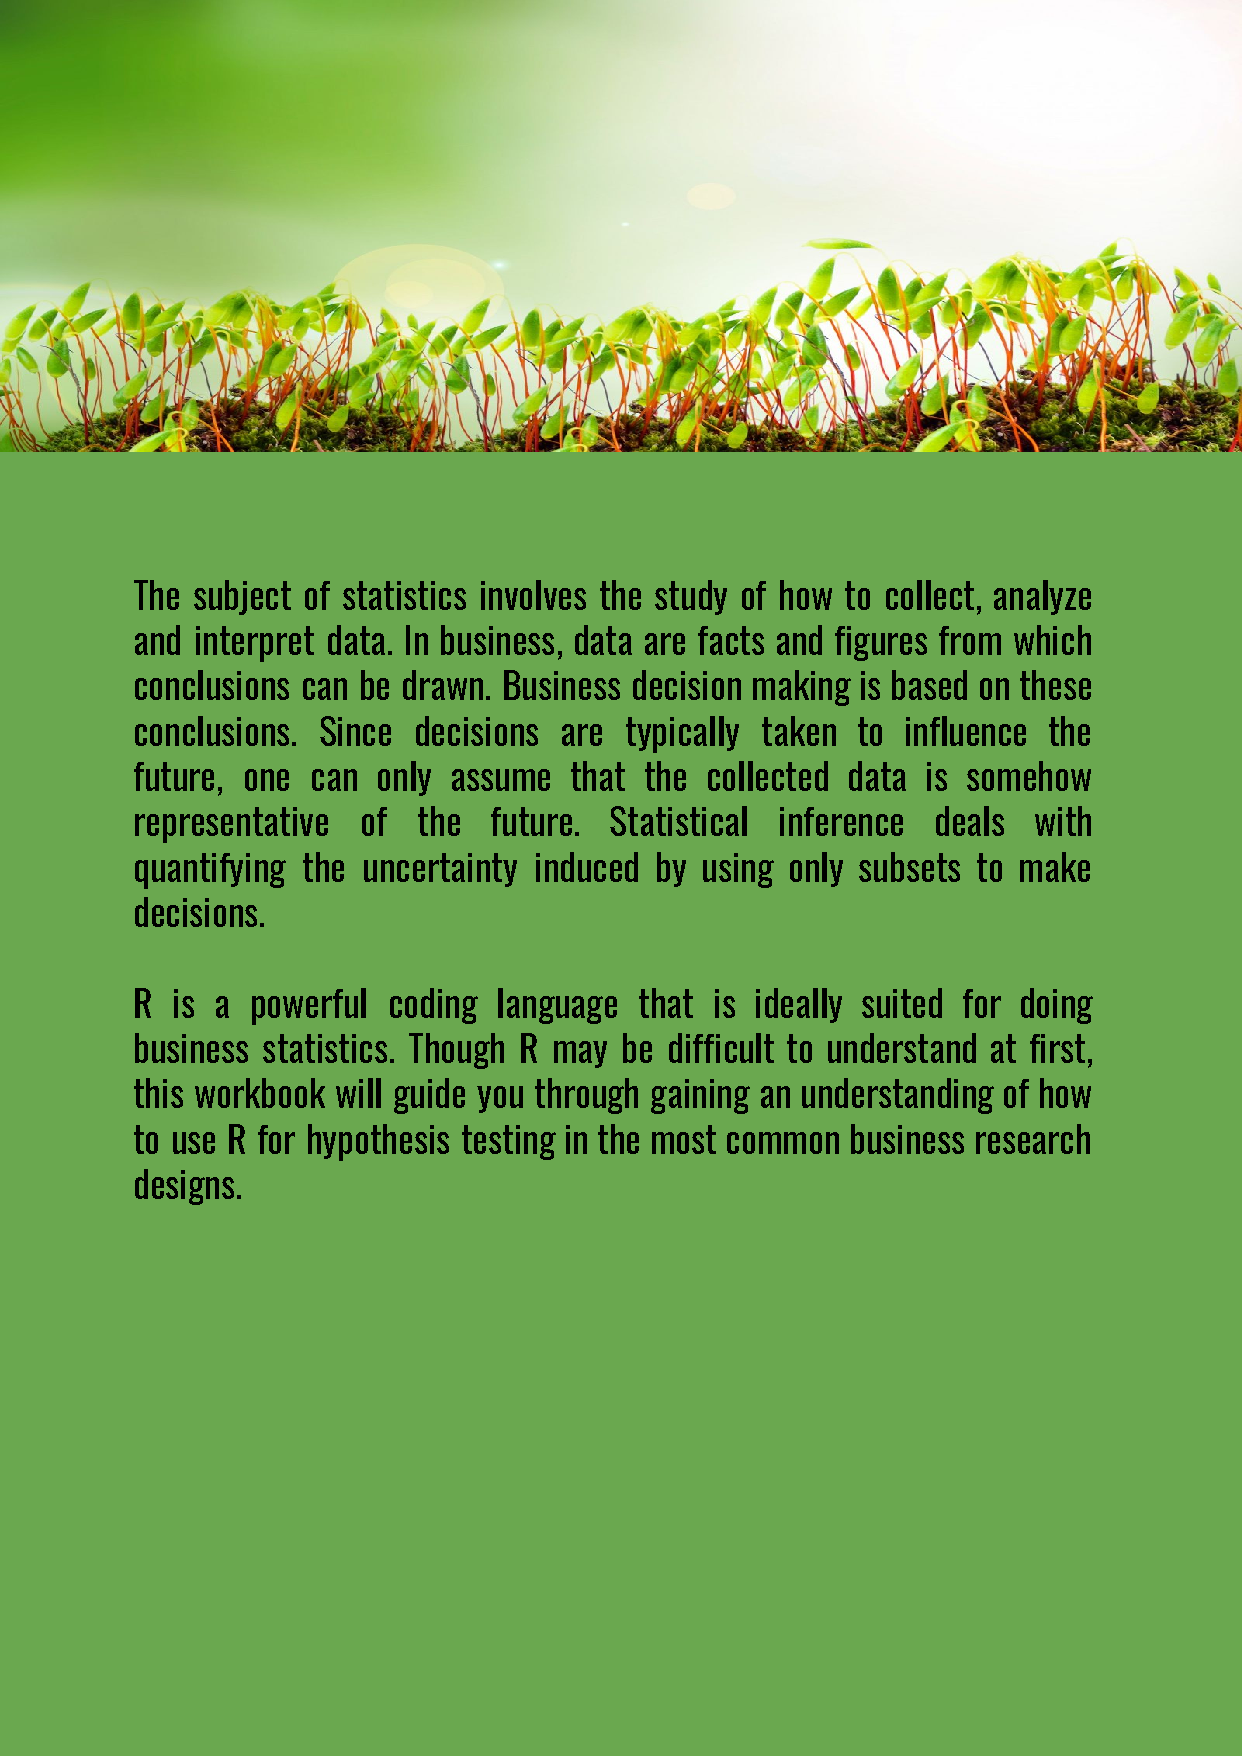
\includepdf[scale=1]{Files/3. Back page/Back page.pdf}

\end{document}
